\documentclass[11pt]{amsbook} 

% This is /definitely/ long enough for amsbook.
\usepackage{geometry} \geometry{letterpaper} 

% Begin paragraphs with an empty line rather than an indent
% This causes a warning from LaTeX.
\usepackage[parfill]{parskip} 

% Use strikethrough and underlines
\usepackage{ulem} 

\usepackage{graphicx} 

\DeclareGraphicsRule{.tif}{png}{.png}{`convert #1 `dirname #1`/`basename #1 .tif`.png}



% The AMS packages everyone uses.
\usepackage{amssymb, amsfonts, amssymb, amsthm, amscd} 

% Allow us to use .eps figures
\usepackage{epstopdf} 

% Used for one diagram.  'twill be fixed.
%\usepackage{pictexwd,dcpic} 


% I prefer this diagram package, but it doesn't work with dcpic.
\usepackage[all,2cell]{xy}	

\usepackage{subfigure}


% Various useful environments.  Eventually I'll try to redefine them to look nice(r).
% I'm also not sure whether all of these should be unnumbered like this.

% the default style
\theoremstyle{plain} 
\newtheorem{theorem}{Theorem} 
\newtheorem*{lemma}{Lemma} 
\newtheorem*{corollary}{Corollary}

\theoremstyle{definition} 
\newtheorem*{example}{Example} 
\newtheorem*{definition}{Definition} 
\newtheorem*{smallfact}{Small Fact} 
\newtheorem*{tinyfact}{Tiny Fact}

% Nice shorthand for commonly-used commands.
\newcommand{\R}{\mathbb R} 
\newcommand{\Z}{\mathbb Z} 
\newcommand{\Q}{\mathbb Q} 
\newcommand{\N}{\mathbb N}
\newcommand{\RP}{\mathbb{RP}}

% A couple of useful shortcuts
\newcommand{\interior}[1]{\overset{\circ}{#1}} 
\newcommand{\closure}[1]{\overline{#1}} 
\newcommand{\Int}{\mathrm{Int}} 
\newcommand{\onto}{\twoheadrightarrow}

% The ulem package overrides \emph to be underline.  I don't like that.
\renewcommand{\emph}[1]{\textit{#1}}

% A nice placeholder image.  
%Well, it will be nicer eventually, when it is replace by real pictures.
\newcommand{\placeholder}{\[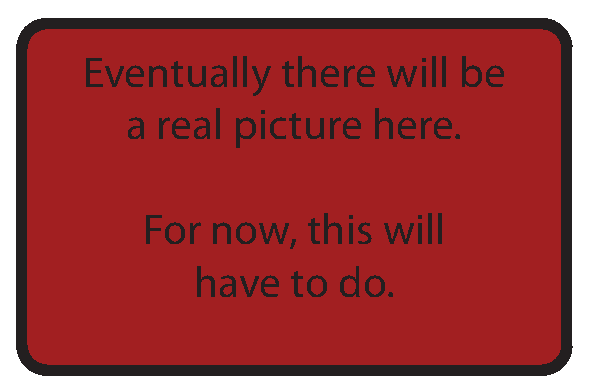
\includegraphics[width=100pt]{images/placeholder}\]}

\title{\LARGE The \sout{Big} Little Book of Topology Notes} 
\author{\Large The Students of Math 147\\
Spring 2010 \\\mbox{ }\\
{\Small Compiled by Daniel Moore}}

\begin{document} 
\maketitle

% To avoid having a 180KB, 3000-line .tex file in which it's impossible to find anything, I split up the text into several smaller files.  
% \input is used because it doesn't use \clearpage and so doesn't make lots of empty pages.


%!TEX root = ../Notes.tex
\chapter{Definitions and Examples} 
\section{Introduction} {\bf What is geometry?} Geometry is the study of rigid shapes that can be distinguished with measurements (length, angle, area, \ldots).

{\bf What is topology?} Topology is the study of shapes which are equivalent via deformations. 

{\bf Topology versus Geometry:} Objects that have the same topology do not necessarily have the same geometry. For instance, a square and a triangle have different geometries but the same topology.
\[ 
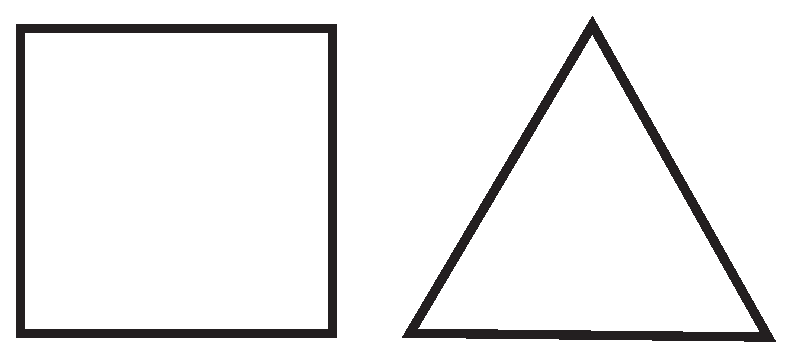
\includegraphics[width=150pt]{images/notes1/square_and_triangle.eps} \]

{\bf Motivation:} Our goal is to understand the shape of our universe. Consider the following examples of two-dimensional universes: a plane, a sphere, a torus, and planes connected by tubes.
\[ 
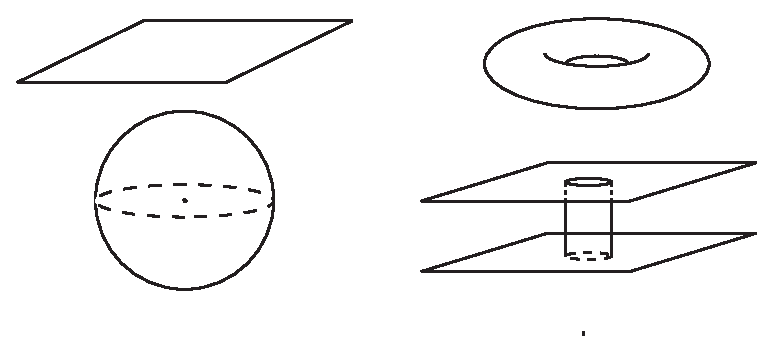
\includegraphics[width=300pt]{images/notes1/various_shapes.eps} \]

\noindent These are topologically distinct universes. Intuitively, we can see that their ``holes'' distinguish them. Hence we seek a mathematical way to describe the holes; one familiar concept we will use is continuity, which is related to a lack of holes.

\section{Some Review from Analysis}
\begin{definition}
	Let $f : \mathbb{R} \rightarrow \mathbb{R}$ and $a \in \mathbb{R}$. We say $f$ is continuous at $a$ if $\forall \epsilon > 0$ $\exists$ $\delta > 0$ such that if $|x-a|<\delta$, then $|f(x)-f(a)|<\epsilon$. 
\end{definition}
\begin{definition}
	Let $M$ be a set and $d: M \times M \rightarrow \mathbb{R}$ be a function such that 
	\begin{enumerate}
		\item $d(a,b)=0$ iff $a=b$ (\textbf{nondegeneracy}) 
		\item $\forall a,b,c \in M$, $d(b,c) \leq d(a,b) + d(a,c)$ (\textbf{triangle inequality}). 
	\end{enumerate}
	Then we say $d$ is a \textbf{metric} or distance and $(M,d)$ denotes a \textbf{metric space}. 
\end{definition}

\noindent Compare this to the usual definition of a metric space. The above definition is equivalent to the usual definition of a metric space, but does not explicitly state the properties of positivity or symmetry: 
\begin{enumerate}
	\item $d(a,b) \geq 0$ $\forall a,b \in M$ (\textbf{positivity}) 
	\item $d(a,b) = d(b,a)$ $\forall a,b \in M$ (\textbf{symmetry}). 
\end{enumerate}
\begin{definition}
	The \textbf{usual metric} on $\mathbb{R}^{n}$ is 
	\begin{displaymath}
		d((x_1,\ldots,x_n),(y_1,\ldots,y_n)) = \sqrt{\sum_{i=1}^n (x_i-y_i)^2}. 
	\end{displaymath}
\end{definition}
\begin{definition}
	Let $M$ be any set. Then the \textbf{discrete metric} is defined as 
	\begin{displaymath}
		d(a,b) = \left\{ 
		\begin{array}{lr}
			1 & \text{if } a \neq b \\
			0 & \text{if } a = b 
		\end{array}
		\right. 
	\end{displaymath}
\end{definition}
The discrete metric can be useful for testing conjectures as it does not rely on $\mathbb{R}^n$.

\pagebreak 
\begin{example}
	{The Comb Metric for $\mathbb{R}^2$.}
\end{example}

Let $X_0 = \{ 0 \} \times [0,1]$, $Y_0 = [0,1] \times \{ 0 \}$; and $\forall n \in \mathbb{N}$, let $X_n = \{ \frac{1}{n} \} \times [0,1]$. Let $M = (\cup_{n=0}^\infty X_n) \cup Y_0$. The distance is the distance measured along the comb in $\mathbb{R}^2$.
\[ 
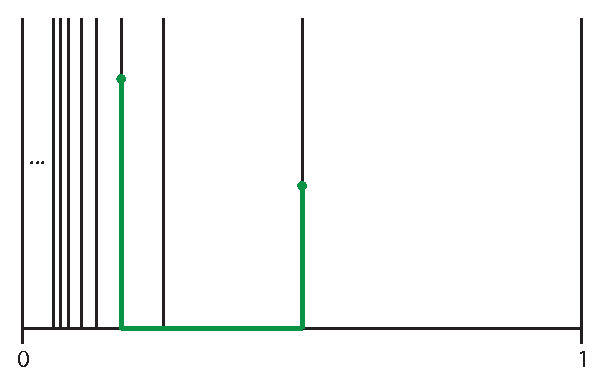
\includegraphics[width=300pt]{images/notes1/comb_space.eps} \]

\noindent Using the comb metric, 
\begin{itemize}
	\item Does the sequence $\{ (\frac{1}{n},0) \}$ converge? Yes, to the origin. 
	\item Does the sequence $\{ (\frac{1}{n},a) \}$ converge when $a \in (0,1]$? No, since $d((\frac{1}{n},a),(0,a)) > 2a$ $\forall n$. 
\end{itemize}
\begin{example}
	{A Non-Example of a Metric Space.} 
\end{example}
Consider the line of real numbers with $d(a,b) = a-b$. Clearly, $d(a,b)=0$ only when $a=b$, satisfying the first property (nondegeneracy). However, the second property (triangle inequality) is not satisfied: if $a=0$, $b=1$, and $c=-1$, then $2=d(b,c) \nleq d(a,b)+d(a,c)=-1+1=0$. Notice that this non-example also fails to satisfy the other two properties listed in the usual definition of a metric, positivity and symmetry.
\begin{example}
	Let $M$ be a set and $d:M\times M\to \R$ a function which satisfies property $2$ but not property $1$ in the definition of a metric space. Then
	\[d(a,b) = 0 \quad \forall a,b \in M\]
	and $M$ has at least 2 points. 
\end{example}
 


%!TEX root = ../Notes.tex
\section{Continuity, metric spaces, and open balls} We'd like to be able to talk about continuity in metric spaces (not just the reals).
\begin{definition}
	Let $(M_1, d_1)$ and $(M_2, d_2)$ be metric spaces and $a \in M_1$. Let $f:M_1 \rightarrow M_2$. We say $f$ is {\bf continuous} at a if $\forall \epsilon > 0$ there exists a $\delta > 0$ such that $\forall x\in M_1$ with $d_1 (x,a) <\delta$ then $d_2 (f(x), f(a))<\epsilon$. 
\end{definition}

%\begin{figure}[ht!]
\[ 
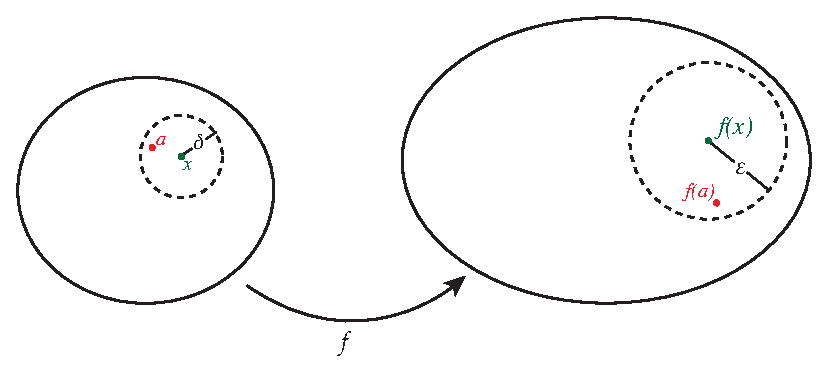
\includegraphics[width=300pt]{images/continuity_etc/continuous_metric_space}\]

%    \caption{For any $a$ such that $d_1(x,a) < \delta$, we have $d_2(f(x), f(a)) < \epsilon$.}
%\end{figure}
\begin{definition}
	Let (M,d) be a metric space and $a\in M$. The {\bf open ball of radius $\epsilon >0$ about $a$} is defined to be
	\[B_\epsilon (a) = \{x\in M\ |\ d(x,a)<\epsilon \}\]
\end{definition}

We can redefine `continuous' in terms of open balls: 
\begin{definition}
	A function $f:X\to Y$ is {\bf continuous} at $a\in X$ iff $\forall\epsilon > 0$ there exists a $\delta >0$ such that if $x\in B_\delta (a)$ then $f(x) \in B_\epsilon (f(a))$.
	
	In other words, $f$ is continuous at $a$ iff for every $\epsilon > 0$ there is some $\delta > 0$ such that $f(B_\delta (a)) \subseteq B_\epsilon (f(a))$. 
\end{definition}

%\begin{figure}[ht!]
\[ 
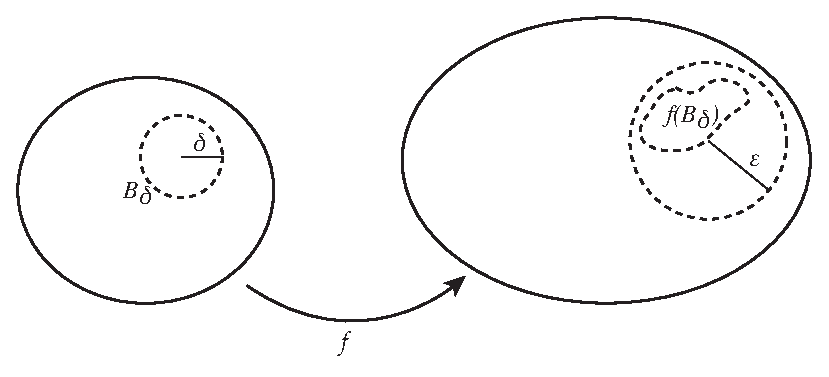
\includegraphics[width=300pt]{images/continuity_etc/continuous_metric_space_balls}\]

%    \caption{For any $\epsilon$, there is some $\delta$ such that $f(B_\epsilon(x))\subseteq B_\delta$.}
%\end{figure}
It should be noted that open balls don't always look like open balls...
\begin{example}
	$M =$ upper half of plane with usual distance
	
	%\begin{figure}[ht!]
	\[ 
	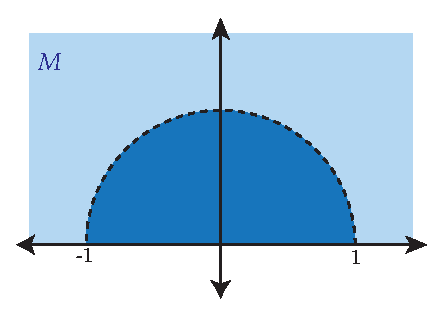
\includegraphics[width=240pt]{images/continuity_etc/upper_half_plane_ex}\]
	
	%    \caption{This half-circle is the intersection of an open set with $M$, so it is open.}
	%\end{figure}
	Because the dark-blue semicircle is the intersection of the open set $\{(x,y)\in\R^2\ |\ x^2+y^2<1\}$ with $M$, it is open in $M$. 
\end{example}
\begin{example}
	In $\R$ with the discrete metric, $B_1 (47) = {47}$ and $B_2 (47) = \R$. 
\end{example}
\begin{example}
	[Comb metric] Under the comb metric, $B_{\frac{1}{2}} ((0,1))$ is just an interval along the y-axis starting at $(0,1)$.
	
	$B_2 ((0,1)$ is everything on the comb below the line of slope $-1$ that connects points $(0,1)$ and $(1,0)$. Since it's an open ball, the line is not contained in the ball.
	\[ 
	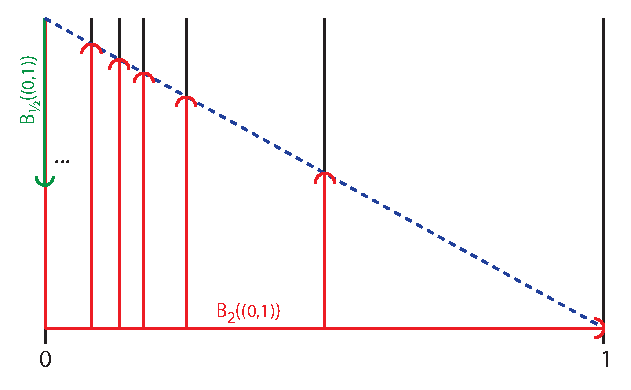
\includegraphics[width=360pt]{images/continuity_etc/comb_metric_balls} \]
\end{example}

Note: Balls are not closed under $\bigcup$ and $\bigcap$ - in $\R^2$, $B_{1}((0,0)) \cap B_{1/2}((1,0))$ and $B_{1}((0,0))\cup B_{1/2}((1,0))$ are not balls.

\section{Open sets} 
\begin{definition}
	Let $(M,d)$ be a metric space. A set $U \subseteq M$ is said to be {\bf open} if $\forall a\in U$ there exists an $\epsilon >0$ such that $B_\epsilon (a) \subseteq U$. 
\end{definition}
\begin{example}
	Every subset of a set $M$ under the discrete metric is open.
\end{example}

\mbox{ }
\begin{smallfact}
	In a metric space, open balls are open sets. 
\end{smallfact}
\proof{ Let $a \in M$ and $\epsilon >0$. We want to show that $B_\epsilon (a)$ is open. That is, we want to show that $\forall x \in B_\epsilon (a)$ there exists an $r>0$ such that $B_r (x) \subseteq B_\epsilon (a)$.

Let $x \in B_\epsilon (a)$ and let $r < \epsilon - d(x,a)$ and $r > 0$. We claim that $B_r (x) \subseteq B_\epsilon (a)$. 

Let $y \in B_r (x)$. Then $d(y,a)\leq d(y,x) + d(x,a) < \epsilon - d(x,a) + d(x,a)= \epsilon$.

Therefore, $B_r (x) \subseteq B_\epsilon (a)$ }
\begin{definition}
	Let
	\[\bigcup_{i \in I} U_i = \{x \in U_i\ |\ i \in I\}\]
\end{definition}
\pagebreak
\begin{theorem}
	(the ``open sets are nice" theorem)
	
	Let $F$ be the family of open sets in a metric space $(M,d)$. Then: 
	\begin{enumerate}
		\item $M$, $\emptyset \in$ $F$ 
		\item If U, V $\in$ F then U $\cap$ V $\in$ F 
		\item If $\forall i \in I$, $U_i \in F$ then $\bigcup_{i \in I} U_i \in F$ 
	\end{enumerate}
\end{theorem}
\begin{proof}
	\begin{enumerate}
		\item Let $x\in M$, and $\epsilon = 47$. By definition,
		\[B_{47} (x) = \{y\in M\ |\ d(x,y)<47\} \subseteq M\]
		Also, trivially $\forall x\in \emptyset$ there exists an $\epsilon > 0$ such that $B_\epsilon (x) \subseteq \emptyset$. Therefore, $M$ and $\emptyset$ are open, and so $M, \emptyset\in F$.
		
		\item Let $x\in U\cup V$, let $r_1 >0$ such that $B_{r_1} (x) \subseteq U$, and let $r_2 >0$ such that $B_{r_2} (x) \subseteq V$. Let $r = \min\{r_1, r_2 \}$. Then clearly $B_r (x) \subseteq B_{r_1} (x) \subseteq U$ and $B_r (x) \subseteq B_{r_2} (x) \subseteq V$. Thus $B_r (x) \subseteq U \cap V$ as desired.
		
		\item Let $x \in \bigcup_{i\in I} U_i$. We want to show that there exists an $r>0$ such that $B_r (x) \subseteq \bigcup_{i\in I} U_i$. 
		
		Because $x\in \bigcup_{i\in I} U_i$, there exists an $i_0 \in I$ such that $x\in U_{i_0}$. Then there must exist an $r>0$ such that $B_r (x) \subseteq U_{i_0}$. Then
		\[B_r (x) \subseteq U_{i_0} \subseteq \bigcup_{i\in I} U_i\]
		and hence $\bigcup_{i\in I} U_i\in F$. 
	\end{enumerate}
\end{proof}
\begin{definition}
	If $f:X \to Y$ and $U \subseteq Y$ then $f^{-1} (U) = \{x\in X\ |\ f(x) \in U\}$. 
\end{definition}
\begin{theorem}
	Let $(M_1, d_1)$ and $(M_2, d_2)$ be metric spaces and $f: M_1 \to M_2$. Then $f$ is continuous if and only if for every $U \subseteq M_2$ that is open in $(M_2, d_2)$, $f^{-1} (U)$ is open in $(M_1, d_1)$. 
\end{theorem}
\begin{proof}
	\begin{itemize}
		\item[$(\Rightarrow)$] Suppose $f$ is continuous. Let $U \subseteq M_2$ be open. We want to show that $\forall x \in f^{-1} (U)$ there exists an $r>0$ such that $B_r (x) \subseteq f^{-1} (U)$.
		
		Let $x\in f^{-1} (U)$. Since $f(x)\in U$ and $U$ is open, there exists $\epsilon >0$ such that $B_\epsilon (f(x)) \subseteq U$. Since $f$ is continuous there exists an $r>0$ such that
		\[f(B_r (x)) \subseteq B_\epsilon (f(x)) \subseteq U\]
		
		Thus, $f^{-1} (f(B_r (x))) \subseteq f^{-1} (U)$. Therefore $B_r (x) \subseteq f^{-1} (f(B_r (x))) \subseteq f^{-1} (U)$ as desired.
		
		\item[$(\Leftarrow)$] Suppose that for all open $U\subseteq M_{2}$, $f^{-1}(U)$ is open in $M_{1}$. Let $p \in M_{1}$. We want to show that $f$ is continuous at $p$.
		
		Let $\epsilon > 0$. $B_{\epsilon}(f(p))$ is open, so $f^{-1}(B_{\epsilon}(f(p)))$ is open. $p\in f^{-1}(B_{\epsilon}(f(p)))$, so $\exists$ $\delta>0$ such that $B_{\delta}(p)\subseteq f^{-1}(B_{\epsilon}(f(p)))$.
		
		$f(B_{\delta}(p))\subseteq f(f^{-1}(B_{\epsilon}(f(p))))=B_{\epsilon}(f(p))$, so $f$ is continuous at $p$, and thus everywhere. $\blacksquare$ 
	\end{itemize}
\end{proof}

We've proven a small fact: 
\begin{smallfact}
	If $f : M_{1} \rightarrow M_{2}$, then $f$ is continuous if for all $p\in M_{1}$, and for all $\epsilon>0$ $f^{-1}(B_{\epsilon}(f(p)))$ is open. 
\end{smallfact}
 


%!TEX root = ../Notes.tex
\section{Topologies} We haven't actually defined what a topology is yet. Let's fix that.
\begin{definition}
	Let $X$ be a set and $F$ be some collection of subsets of $X$ such that
	
	$1)$ $X,\emptyset \in F$.
	
	$2)$ If $U,V \in F$ then $U\cap V \in F$ .
	
	$3)$ If for all $i\in I$, $U_{i} \in F$, then $\bigcup U_{i} \in F$.
	
	Then we say that $(X,F)$ is a {\bf topological space} with {\bf open sets} the elements of $F$. We also say $F$ is the {\bf topology} on $X$. 
\end{definition}
\begin{example}
	Let $(M,d)$ be a metric space and $F$ be the set of open sets in $M$. Then $(M,F)$ is a topological space. 
\end{example}
\begin{definition}
	Let $M$ be a set and $d$ be the discrete metric, then we say $(M,F)$ is the {\bf discrete topology}. 
\end{definition}
\begin{definition}
	Let $X$ be a set with at least 2 points. Let $F=\{X,\emptyset\}$. Then we say $(X,F)$ is the {\bf indiscrete}, or {\bf concrete} topology. 
\end{definition}
\begin{definition}
	If $F_{1}$ and $F_{2}$ are topologies on $X$ and $F_{1}\subseteq F_{2}$ then we say that $F_{1}$ is {\bf weaker} than $F_{2}$, or $F_{2}$ is {\bf stronger} than $F_{1}$. 
\end{definition}

Two notes: 
\begin{itemize}
	\item weaker = fewer = coarser and stronger = more = finer. 
	\item The discrete topology is the strongest topology on $M$ and the indiscrete topology is the weakest topology on $X$. 
\end{itemize}
\begin{example}
	Let $X=R$ and $U\in F$ iff $U$ is the union of sets of the form $[a,b)$ such that $a,b\in \mathbb{R}$. (This is called the {\bf half-open interval topology}). 
\end{example}

Is this weaker, stronger, or neither compared to the usual topology?

If the interval $(a,b) \in F$, then $F$ is stronger. Let $a,b \in \mathbb{R}$, and $a<b$. Then, $(a,b)=\bigcup_{n\in \mathbb{N}}[a+\frac{1}{n},b)$, so $F$ is stronger.
\begin{example}
	Let $X=\mathbb{R}^{2}$ have the "dictionary order". This means that $(a,b)<(c,d)$ if either $a<c$ or a=c and $b<d$. 
\end{example}

Note that $U\in F$ iff $U$ is a union of ``open intervals", i.e. $\{(x,y)\ |\ (a,b)<(x,y)<(c,d)\}$.
\begin{itemize}
	\item Is a vertical line open? Yes. 
	\item Is a horizontal line open? No. 
	\item Is this topology finer or coarser than the usual topology on $\mathbb{R}^{2}$?
	
	Well, any point in a ball in the usual topology can be found in a ball of the dictionary topology, which is contained in the usual ball. Open balls are open in the dictionary topology, so the dictionary topology is finer than the usual topology. 
\end{itemize}

Note: In $\mathbb{R}$, $\bigcup_{n\in \mathbb{z}}(n,n+1)$ is open.

\mbox{ }

$Question$: Are the topologies on a set linearly ordered? No! 
\begin{example}
	Consider $\R$ with the usual topology and $(\R, F)$ with $F = \left\{ \R, \phi,47 \right\}$. We say these two topologies are {\bf incomparable}. 
\end{example}
\begin{example}
	Consider $(\mathbb{R},F)$ Define $U \in F$ if and only if either $U=\phi$ or $U=\mathbb{R}$, or $\mathbb{R}-U$ is finite. We see that if $U$ is open in $(\mathbb{R},F)$, then U is open in the usual topology. Therefore the usual topology is finer. This topology is called the {\bf finite complement topology on $\mathbb{R}$}. 
\end{example}
\begin{definition}
	A set $C$ in a topological space $(X,F)$ is {\bf closed} iff its complement $X\setminus C$ is open. 
\end{definition}

Note that a set can be both open and closed as well as neither open nor closed. (It is not a door!)
\begin{example}
	Let us consider $\mathbb{R}$ with the half-open interval topology. Then $[ 0,\infty) =\bigcup _{n \in \N} [0,n)$ is open. On the other hand, the complement of this set is $(-\infty,0) =\bigcup_{n \in\N } [-n,0)$, which is also open. Thus this is a {\bf clopen} set. 
\end{example}
\begin{example}
	A ``vertical line" in $\mathbb{R}^{2}$ with the dictionary order is both open and closed. The proof is left as exercise. 
\end{example}
\begin{lemma}
	Let $(X,F)$ be a topological space and $A$ be the set of all closed sets in X. Then: 
	\begin{enumerate}
		\item $X,\phi \in A$ 
		\item If $C,D \in A$, then $C \bigcap D \in A$ 
		\item If $C_i \in A$ for every $i \in I$, then $\bigcap_{i\in I}C_i \in A$ 
	\end{enumerate}
\end{lemma}
The proof is basically the same as that for open sets back in section 4.
\begin{definition}
	Let $(X,F)$ be a topological space and $A \subseteq X$. Let $\{ U_j\ |\ j \in J \}$ be the set of all open sets contained in $A$. Then we define $\interior{A} = \mathrm{Int}(A) = \bigcup_{j \in J} U_j$, and we say $\interior{A}$ is the {\bf interior} of $A$. 
\end{definition}
\begin{smallfact}
	Let $(X,F)$ be a topological space and $A \subseteq X$. Then 
	\begin{enumerate}
		\item $\interior A \subseteq A$ 
		\item $\interior A$ is open 
		\item If $U\subseteq A$ is open, then $U\subseteq \interior A$ 
		\item $A$ is open iff $A = \interior A$. 
	\end{enumerate}
\end{smallfact}
\begin{proof}
	\begin{enumerate}
		\item Since $\interior A = \bigcup_{j\in J} U_j$ and $U_j \subseteq A$ for every $j \in J$, $\interior A\subseteq A$. 
		\item By definition, $\interior A$ is a union of open sets, so $\interior A$ is open. 
		\item Since $U$ is open in $A$, $U \in \{ U_j\ |\ j\in J\}$. Therefore $U\subseteq \bigcup_{j\in J} U_j = \interior A$. 
		
		Note that this means that $\interior A$ is the ``largest'' open set in $A$. 
		\item Suppose that $A = \interior A$. Then $\interior A$ is open by part (2), hence $A$ is open.
		
		Conversely, suppose that $A$ is open. Then $A\in \{U_j\ |\ j\in J\}$. Hence $A \subseteq \interior A$. From (1), $A = \interior A$. 
	\end{enumerate}
\end{proof}
\begin{example}
	In the half-open interval topology on $\R$, $\Int((0,1])=(0,1)$. To prove this, assume that $1\in \Int((0,1])$ and show that it leads to a contradiction. 
\end{example}
\begin{example}
	In the finite-complement topology on $\R$, $\Int((0,1])= \emptyset$. This follows from the fact that $\R$ is infinite and all subsets of $(0,1]$ are finite. 
\end{example}
\begin{example}
	In the dictionary-order topology on $\R^2$, $\Int( [ 0,1] \times [ 0,1] ) = [0,1] \times (0,1)$. \placeholder 
\end{example}
\begin{definition}
	Let $A$ be a subset of a topological space $(X,F)$, and let $\{ F_j\ |\ j \in J \}$ be the set of all closed sets containing $A$. Then the {\bf closure} of $A$ is defined as $\closure{A} = cl(A) = \bigcap_{j \in J}F_j$. 
\end{definition}
\begin{smallfact}
	Small facts about closures: 
	\begin{enumerate}
		\item $A \subseteq \closure{A}$ 
		\item $\closure{A}$ is closed 
		\item If $A \subseteq C$ and $C$ is closed, then $\closure{A}\subseteq\closure{C}$ 
		\item $\closure{A}=A$ if and only if $A$ is closed. 
	\end{enumerate}
\end{smallfact}
The proofs are left as exercises.
\begin{example}
	In $\R$ with the usual topology, $\mathrm{cl}\left(\left\{ \frac{1}{n}|n \in \N \right\}\right) = \left\{\frac{1}{n}|n \in \N \right\} \cup \{ 0\}$ 
\end{example}
\begin{example}
	In $\R$ with the half-open interval topology, $\mathrm{cl}((0,1])=[ 0, 1]$ 
\end{example}
\begin{lemma}
	(an Important Lemma)\\
	Let $(X,F)$ be a topological space and $Y \subseteq X$. Then $ p \in \closure{Y}$ if and only if for every open set $U\subseteq X$ containing $p$, $U \cap Y \neq\emptyset$. 
\end{lemma}
\begin{proof}
	Let $p \in \closure{Y}$ and $U\subseteq X$ be open with $p \in U$. Suppose $U \cap Y = \emptyset$ and let $C=X\setminus U$. Then $p\notin C$ because $p \in U$. It follows that $\overline{Y} \subseteq C$ because $Y \subseteq C$ and $C$ is closed. We obtain that $p \in C$, which is a contradiction.
	
	Conversely, suppose that for every open set $U\subseteq X$ such that $p \in U$, $U\cap Y \neq \emptyset$. Let $C\subseteq X$ be closed such that $Y \subseteq C$. Suppose $p \notin C$. Let $U=X\setminus C$, which is open with $p \in U$. Now $U \cap Y \neq\emptyset$, so there exists some $x \in U \cap Y$. This means that $x\in X\setminus C$, i.e. $x \notin C$. But since $Y \subseteq C$, we have $x \notin Y$, a contradiction. Therefore we conclude that $p \in \closure{Y}$. 
\end{proof}
\begin{corollary}
	Suppose that $U$ is an open set in a topological space $(X,F)$ and $Y \subseteq X$. If $U \bigcap \closure{Y}\neq\emptyset$, then $U \bigcap Y \neq \emptyset$. 
\end{corollary}

\proof The proof is immediate from the important lemma.

Now we can use the important lemma to prove that in $\R$ in the usual topology, $\mathrm{cl}(\{1/n\ |\ n\in\N\}) = \{1/n\ |\ n\in\N\}\cup\{0\}$. Here, we can show that for all open sets $U$ containing 0, $U \bigcap\left\{ \frac{1}{n}\ |\ n \in \mathbb{N} \right\} \neq \emptyset$.
 


%!TEX root = ../Notes.tex
\section{Continuity in Topological Spaces} 
\begin{definition}
	Let $(X_1,F_1)$ and $(X_2,F_2)$ be topological spaces and $f: X_1 \to X_2$. We say $f$ is {\bf continuous} if and only if for every $U \in F_2$, $f^{-1}(U)\in F_1$. 
\end{definition}
\begin{smallfact}
	Let $(X_1,F_1)$ and $(X_2,F_2)$ and $(X_3,F_3)$ be topological spaces, $f: X_1 \to X_2$ and $f: X_2 \to X_3$ be continuous functions. Then $g \circ f: X_1 \to X_3$ is continuous. 
\end{smallfact}
\begin{proof}
	Let $U \in F_3$. Then $g^{-1}(U) \in F_2$ because $g$ is continuous, and $f^{-1}(g^{-1}(U)) \in F_1$ because $f$ is continuous. Therefore $(g \circ f)^{-1}(U) \in F_1$. Thus $g\circ f$ is continuous. 
\end{proof}
\begin{theorem}
	Let $X$, $Y$ be topological spaces and $f: X \to Y$. Then $f$ is continuous if and only if for every closed set C in Y, $f^{-1}(C)$ is closed in X. 
\end{theorem}
\begin{itemize}
	\item [$(\Rightarrow)$] Suppose $C$ is closed in $Y$. Then $Y\setminus C$ is open, implying that $f^{-1}(Y\setminus C)$ is open in $X$. Since $f^{-1}(Y\setminus C)= \{ x \in X\ |\ f(x) \in Y\setminus C\} = \{ x \in X\ |\ f(x) \notin C \}$ and $X\setminus f^{-1}(C)= \{ x \in X\ |\ f(x) \notin C \}$, we have the desired results. 
	\item [$\Leftarrow$] This is exactly like the analogous proof for open sets. 
\end{itemize}

This is nice, because sometimes it's easier to work with closed sets than with open sets. 
\begin{definition}
	Let $X$ and $Y$ be topological spaces, and let $f:X\to Y$. 
	\begin{enumerate}
		\item If for every open set $U\subseteq X$, $f(U)$ is open in $Y$, then $f$ is {\bf open}. 
		\item If for every closed set $U\subseteq X$, $f(U)$ is closed in $Y$, then $f$ is {\bf closed}. 
	\end{enumerate}
\end{definition}

This is sort of like continuity, except that we care about the image of sets instead of their preimages.

Example time! 
\begin{example}
	Let $F$ be the half-open topology on $\R$, and define a function
	\[{f:(\R,F)\to(\R,\text{usual})}\qquad\text{ by }f(x) = x\]
\end{example}
\begin{itemize}
	\item Is $f$ continuous? Yes! An open set in $(\R, \text{usual})$ is a union of intervals of the form $(a,b)$. We know that $f^{-1}\big((a,b)\big) = (a,b)$, which is open in $F$. 
	\item Is $f$ open? No. Take any $U = [a,b) \in F$. Then $f(U) = [a,b)$, which is not open in $(\R, \text{usual})$. 
	\item Is $f$ closed? Also no, since $f\big([a,b)\big) = [a,b)$ is not closed in $(\R, \text{usual})$. 
\end{itemize}

\section{Homeomorphisms} Let's define a notion of equivalency for topological spaces. 
\begin{definition}
	Let $(X_1,F_1)$ and $(X_2,F_2)$ be topological spaces, and let $f:X_1\to X_2$ be continuous, bijective, and open. Then $f$ is a {\bf homeomorphism}, and $X_1$ and $X_2$ are {\bf homeomorphic} (denoted by $X_1 \cong X_2$). 
\end{definition}
\begin{example}
	Let $I = [0,1]$ and $X = I\times I\subset\R^2$, under the usual metric for $\R^2$. Let \nobreak{$Y = \{ (x,y)\in\R^2 | x^2+y^2\le 1\} = D^2$} be the unit disk in $\R^2$. Question: Are $X$ and $Y$ homeomorphic? 
	
	Answer: Yes! Let's see how. 
\end{example}

Define the centers of $X$ and $Y$ to be $x$ and $y$, respectively. Fix some point $a$ on the boundary of $X$, and some $b$ on the boundary of $Y$ (that is, $a\in 
\partial X$ and $b\in\partial Y$).

Define a function $f$ as follows: 
\begin{itemize}
	\item $f(x) = y$ 
	\item $f(a) = b$ 
	\item For $t\in 
	\partial X$, look at the distance along the boundary from $a$ to $t$. Then $f(t)$ is a point proportionally far along the boundary of $Y$. 
	\item For $s\in \text{int}(X)$, draw the ray connecting $x$ and $s$. Let $t$ be the point at which this ray intersects $ 
	\partial X$. Now, in $Y$, draw the ray connecting $y$ and $f(s)$. Then $s$ is mapped to a point on this ray that is proportionally far from $y$. 
\end{itemize}
The last two, in pictures:
\[ 
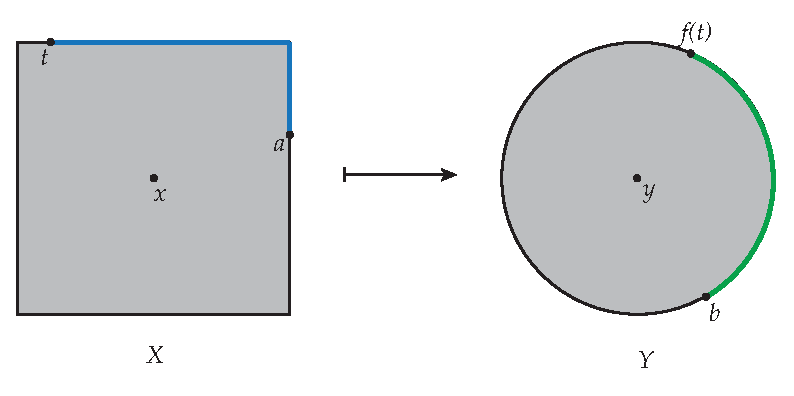
\includegraphics[width=360pt]{images/continuity_and_topology/square_circle_map_1}\]
\[ 
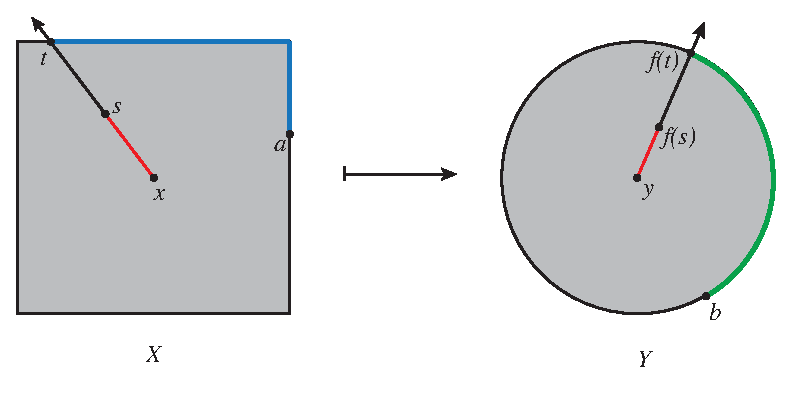
\includegraphics[width=360pt]{images/continuity_and_topology/square_circle_map_2}\]
\begin{itemize}
	\item Is this well-defined? 
	\begin{itemize}
		\item Yes! There is always exactly one point in $Y$ that can be mapped to be a point in $X$\footnote{This works because both a square and a circle are \emph{convex} shapes - for example, for all points $p,q\in X$, the line $\overline{pq}$ that connects $p$ and $q$ lies entirely within $X$. This also implies that $x$ and $y$ didn't actually have to be the exact \emph{centers} of $X$ and $Y$ respectively.}. 
	\end{itemize}
	\item Is this a bijection? 
	\begin{itemize}
		\item Yes! The inverse is defined identically, so it would make sense for this to be a bijection. Also, consider the images of concentric squares centered on $x$ under $f$: they are mapped to disjoint concentric circles centered on $y$. 
	\end{itemize}
	\item Is $f$ continuous and open? 
	\begin{itemize}
		\item Yes! Intuitively, it's easy to see that an open set in $X$ is mapped to an open set in $Y$, and that the preimage of an open set in $Y$ is open. 
	\end{itemize}
\end{itemize}

Question: Can we extend this to (some) non-convex regions? 

Answer: Sure. Just divide up the non-convex region into smaller regions. Actually, a subregion will work as long as there is some point in its interior such that any ray from that point intersects the subregion's boundary exactly once.

However, there are limits to this: for example, a donut is \emph{not} homeomorphic to a circle. This is hard to show; we'll see a proof later.

There are also some homeomorphisms that we might find unsettling. For example, a knot in $\R^3$ and the unit circle $S^1 = \{ (x,y)\in\R^2 | x^2+y^2 = 1\}$ are homeomorphic; the argument works exactly like the one used for $ 
\partial X$ when showing that a square and circle are homeomorphic (above). It turns out that, while the knot and circle are homeomorphic, their complements are not. 
\begin{example}
	Define a function $f:[0,1)\to S^1$ by
	\[ f(t) = \big( \cos(2\pi t), \sin(2\pi t)\big) \]
\end{example}
This takes the interval and wraps it counterclockwise around the circle. 
\begin{itemize}
	\item Is this a bijection? 
	\begin{itemize}
		\item Yes! The interval wraps once around the circle; one end is open, so there is no overlap. 
	\end{itemize}
	
	\item Is $f$ continuous? 
	\begin{itemize}
		\item Yes! First we define an open ball in $S^1$ as $B_{\epsilon, S^1}(a) = \{x\in S^1\ |\ d(x,a) < \epsilon\}$. Then the preimage of every open ball in $S^1$ is an open interval, so $f$ is continuous. 
	\end{itemize}
	
	\item Is $f$ open? 
	\begin{itemize}
		\item No. Let $U = [0, 1/2)$, which is open in $[0,1)$. Sadly, its image is not open in $S^1$. 
	\end{itemize}
\end{itemize}
So this $f$ is not a homeomorphism.

\mbox{ }

We will show that $\R^2 \not\cong \R^3$ near the end of Chapter 3. This is difficult. 
\begin{example}
	Some non-examples of homeomorphisms: 
\end{example}
\begin{itemize}
	\item $\Q$ under the usual topology is not homeomorphic to $\R$ under the usual topology, since there is no bijection between $\Q$ and $\R$. 
	\item $\R$ with the finite-complement topology ($FCT$) is not homeomorphic to $\R$ with the usual topology: 
	\begin{itemize}
		\item Suppose that there is some homeomorphism $f:(\R, FCT)\to(\R,\text{usual})$. Let $U = (0,1)$. 
		\item Look at $f^{-1}(U)$ - it must be open, since $f$ is a homeomorphism. 
		\item It is definitely not equal to $\emptyset$, since $U\ne\emptyset$. 
		\item It is also not $\R$, since $f$ is a bijection. 
		\item So $\R\setminus f^{-1}(U)$ must be finite. But $\R\setminus U$ is not finite. 
		\item Because $f$ is a bijection, this is a contradiction. 
		\item Therefore, $(\R, FCT) \not\cong (\R, \text{usual})$. 
	\end{itemize}
\end{itemize}
 


%!TEX root = ../Notes.tex
\section{Subspaces}
\begin{definition}
	Let $(X, F_X)$ be a topological space, and let $Y\subseteq X$. Let $F_Y = \{U \cap Y | U\in F_X\}$. Then $F_Y$ is the {\bf subspace topology} or {\bf induced topology} on $Y$. 
\end{definition}
\begin{example}
	Consider the topological space $\R^2$ with the dictionary order. 
\end{example}

Q: What are the open sets in the subspace $\Z \times \Z$?\\
A: All sets are open. We can draw a small open interval about any point, so the set of any one point is open, and any set is the union of such sets. Because of all sets are open, we can consider this topology the discrete topology on $\Z \times \Z$.

Example: consider $\Z \times \Z$ as a subspace of $\R^2$, but this time with the usual topology. Again, all sets are open, as we can construct an open ball of radius $\frac12$ about any point that doesn't intersect any others in the same way that we can construct an open interval.

Small facts about subspaces:

Let $(X, F_X)$ and $(Y, F_Y)$ be topological subspaces with $(S, F_S)$ a subspace of $X$ and $(T, F_T)$ a subspace of $Y$. Then 
\begin{enumerate}
	\item If $S\in F_X$, then $F_S \subseteq F_X$. 
	\item $C\le S$ iff $\exists$ a closed set $A$ in $X$ such that $C = A\cap S$. 
	\item Suppose $f:X\to Y$ is continuous. Then $f\ |\ S : S \to Y$ is continuous. 
	\item Suppose $f:X\to Y$ is continuous and $f(X) \subseteq T$. Let $g:X\to T$ be such that $g(x) = f(x) $ for every $x\in X$. Then $g$ is continuous. 
\end{enumerate}

Proofs: 
\begin{enumerate}
	\item If $S \in F_X$, then $S$ is open in $X$. By definition $F_S = \{ U\cap S : U\in F_X\}$ 
	\item 
	\begin{itemize}
		\item [($\Rightarrow$)] Let $C\subseteq S$ be closed. Because $S\setminus C \in F_S$, there is some $U\in F_S$ such that $U\cap S = S\setminus C$. Since $U$ is open in $X$, we know that $X\setminus U$ is closed in $X$. We claim that the closed set we desire is $X\setminus U$. Note that
		\[ X\setminus (U\cap S) = (X\cap S)\setminus (U\cap S) = S\setminus (U\cap S) = S\setminus (S\setminus C) = C\]
		and so we are done 
		\item [($\Leftarrow$)] Suppose that there is a closed set $A\subseteq X$ such that $C = A\cap S$. Then $X\setminus A \in F_X$, so $(X\setminus A)\cap S \in F_S$. But $X\setminus (A\cap S) = (X\cap S)\setminus (A\cap S) = S\setminus C$ is open in $SS$, so $C$ is closed in $S$. 
	\end{itemize}
	\item Let $U\in F_Y$. Since $f$ is continuous, $f^{-1}(U)\in F_X$. Because $(f|S)^{-1}(U) = f^{-1}(U)\cap S$, $(f|S)^{-1}(U)$ is the intersection of an open set with $S$ and so is open. Therefore, $f|S$ is continuous. 
	\item Let $U\in F_T$. Then there is some $V\in F_Y$ such that $U = V\cap T$. Because $f:X\to Y$, $f^{-1}(V)\in F_X$. Since $f(X)\subseteq T$,
	\[ f^{-1}(U) = f^{-1}(V)\cap T = f^{-1}(V\cap T) = f^{-1}(V) \]
	Therefore, $f^{-1}(U)$ is open in $X$. But $f^{-1}(U) = g^{-1}(U)$, so $g^{-1}(U)$ is open and so $g$ is continuous. 
\end{enumerate}

\section{Bases} You may have noticed that, in metric spaces, the idea of open sets was quite useful. We'd like to extend this idea to more general topological spaces.
\begin{definition}
	Let $(X,F)$ be a topological space and $\beta\subseteq F$ such that for every $U\in F$, $U$ is a union of elements in $\beta$. Then we say that $\beta$ is a {\bf basis} for $F$. 
\end{definition}

Note that this basis is not necessarily minimal (like the basis of a vector space), but it {\it is} more useful the more specific it is.
\begin{example}
	$\R$ with the half-open interval topology was {\it defined} by the basis $\big\{ [a, b)\ |\ a < b\big\}$. 
\end{example}
\begin{example}
	$\R^2$ with the dictionary topology was similarly defined by a basis of open intervals. 
\end{example}
\begin{theorem}
	Let $X$ be a set and $\beta$ be a collection of subsets such that 
	\begin{enumerate}
		\item $X = \bigcup_{B\in \beta} B$ 
		\item $\forall B_1, B_2$, if $x\in B_1\cap B_2$, then there is some $B_3\in\beta$ such that $x\in B_3\subseteq B_1\cap B_2$. 
		\item Let $F$ = collection of elements of $\beta$. Then $F$ is a topology on $X$ with basis $\beta$. 
	\end{enumerate}
\end{theorem}
\begin{theorem}
	Let $X$ be a set and $\beta$ a collection of subsets of $X$ such that 
	\begin{enumerate}
		\item $X = \cup_{B \in \beta} B$ 
		\item For all $B_1, B_2 \in \beta$ and $x \in B_1 \cap B_2$, $\exists$ $B_3 \in \beta$ such that $x \in B_3 \subseteq B_1 \cap B_2$. 
	\end{enumerate}
	Let $F = \{$unions of elements of $\beta \}$. Then $F$ is a topology for $X$ with basis $\beta$. 
\end{theorem}
\begin{proof}
	First we prove that $F$ is a topology for $X$. 
	\begin{enumerate}
		\item Since $X = \displaystyle{\cup_{B \in \beta} B}$, by definition $X \in F$. Since $\emptyset$ is the union of zero elements of the $\beta$, we also have $\emptyset \in F$. 
		\item Let $U, V \in F$. Hence we know that there exist index sets $I$ and $J$ such that $U = \cup_{i \in I}B_i$ and $V = \cup_{j \in J}B_j$. Consider $U \cap V = ( \cup_{i \in I}B_i) \cap (\cup_{j \in J}B_j)$. Let $x \in U \cap V$. Then there exists $i_x \in I$ and $j_x \in J$ such that $x \in B_{i_x} \cap B_{j_x}$. From our second assumption we know there exists a $B_x \in \beta$ such that $x \in B_x \subseteq B_{i_x} \cap B_{j_x}$. Let $W = \cup_{x \in U \cap V} B_x$. Since $W$ is a union of elements of $\beta$ it is clearly in $F$. \\
		WTS: $W = U \cap V$\\
		$(\supseteq)$ For all $x \in U \cap V$, we know that $x \in B_x \subseteq \cup_{x \in U \cap V}B_x = W$. Therefore $U \cap V \subseteq W$. \\
		$(\subseteq)$ For all $x \in U \cap V$, we have a $B_x \subseteq B_{i_x} \cap B_{j_x} \subseteq U \cap V$. Therefore, $W = \cup_{x \in U \cup V} B_x \subseteq U \cap V$.\\
		We have containment in both directions, so $W = U \cap V$. 
		\item Suppose $\forall k \in K$, $U_k \in F$. \\
		WTS: $\cup_{k \in K}U_k \in F$. \\
		For all $k \in K$, $U_k = \cup_{i \in I_k} B_i$. Hence $\cup_{k \in K}U_k = \cup_{k \in K} (\cup_{i \in I_k} B_i) \in F$, since it is a union of elements of $\beta$. 
	\end{enumerate}
	Therefore $F$ is a topology. By definition, $\beta$ is also a basis of $F$. 
\end{proof}
\begin{smallfact}
	Let $(X, F_X)$ and $(Y, F_Y)$ be topological spaces with bases of $\beta_X$ and $\beta_Y$ respectively, and $f: X \to Y$. 
	\begin{enumerate}
		\item $f$ is continuous iff $\forall$ $B \in \beta_Y$, $f^{-1}(B) \in F_X$. 
		\item $f$ is open iff $\forall$ $B \in \beta_X$, $f(B) \in F_Y$. 
	\end{enumerate}
\end{smallfact}
\begin{proof}
	(of (1) only. (2) is virtually identical.)\\
	$(\Rightarrow)$ Suppose $f$ is continuous. Then $\forall$ $U \in F_Y$, $f^{-1}(U) \in F_X$ by the definition of continuity. In particular, if $B \in \beta_y$, then $B \in F_Y$ and $f^{-1}(B) \in F_X$. \\
	$(\Leftarrow)$ Suppose $B \in \beta_Y$ implies $f^{-1}(B) \in F_X$. Let $U \in F_Y$. Hence $U = \cup_{i \in I} B_i$ for some index set $I$. Therefore, $$f^{-1}(U) = f^{-1}(\cup_{i \in I} B_i) = \cup_{i \in I} f^{-1}(B_i) \in F_X,$$ since we know $f^{-1}(B_i) \in F_X$ for all $i$ and unions of elements of $F_X$ are in $F_X$. 
\end{proof}
 


%!TEX root = ../Notes.tex
\chapter{Making new spaces from old} 
\section{Quotient Spaces}

First we will consider quotients of sets. 
\begin{definition}
	Let $X$ be a set and $\sim$ a relation on $X$. We say $\sim$ is an {\bf equivalence relation} if 
	\begin{enumerate}
		\item $\forall$ $x \in X, \ x\sim x$ (reflexivity) 
		\item $\forall \ x, y \in X$ if $x\sim y$ then $y\sim x$ (symmetry) 
		\item If $x, y, z \in X$ and $x\sim y$ and $y\sim z$, then $x\sim z$ (transitivity) 
	\end{enumerate}
\end{definition}
\begin{definition}
	Let $X$ be a set with an equivalence relation $\sim$. Then $\forall \ a \in X$ define the {\bf equivalence class} of $a$ as
	\[[a] = \{x \in X : x\sim a \}.\]
\end{definition}
\begin{definition}
	Let $X$ be a set with an equivalence relation $\sim$. Then the {\bf quotient} of $X$ by $\sim$ is
	\[X / \sim = \{ [p] : p \in X\}.\]
\end{definition}
NOTE: The equivalence classes partition $X$ (i.e. $\forall$ $x \in X$, $x \in$ exactly one equivalence class) 
\begin{example}
	Similarity (i.e. $A \sim B$ iff there exists a $P$ such that $A = P^{-1}BP$) is an equivalence relationship on the set of $n \times n$ matrices. However, this is not the ``kind" of equivalence relationships that we will be studying. 
\end{example}
\begin{example}
	Let $X = [0,1]$ and $x\sim y$ iff $x = y$ or $x,y \in \{0,1\}$. This ``glues'' the interval $[0,1]$ into a circle. 
\end{example}
\begin{definition}
	Let $X$ be a set and $\sim$ an equivalence relation. We define $$\pi: X \rightarrow X / \sim$$ such that $\pi(x) = [x] \forall \ x \in X$. We say $\pi$ is the $\mathbf{projection \ map}$. 
\end{definition}
\begin{tinyfact}
	Let $X$ be a set with equivalence relation $\sim$. Then 
	\begin{enumerate}
		\item $\pi$ is onto 
		\item $\pi$ is one-to-one iff ``$\sim$" is ``=". 
	\end{enumerate}
\end{tinyfact}
\begin{proof}
	\begin{enumerate}
		\item Let $[x] \in X / \sim$. Then $\pi(x) = [x]$. Therefore $\pi$ is onto. 
		\item $(\Rightarrow)$ Suppose $\pi$ is one-to-one. Let $x,y \in X$ and $x \sim y$. Then $[x] = [y]$ and $\pi(x) = \pi(y)$, implying $x = y$ since $\pi$ is one-to-one.\\
		$(\Leftarrow)$ Suppose ``$\sim$" is ``=". Let $x,y \in X$ such that $\pi(x) = \pi(y)$. Then $\{x\} = [x] = [y] = \{y\}$, and $x = y$. 
	\end{enumerate}
\end{proof}

Now we would like to define a topology such that $\pi$ is continuous. 
\begin{definition}
	Let $(X, F_X)$ be a topological space and $\sim$ be an equivalence relation on $X$. We define
	\[F_{\sim} = \{U \subseteq X / \sim : \pi^{-1}(U) \in F_X\}\]
	and call $(X / \sim, F_{\sim})$ the {\bf quotient space} of $X$ with respect to $\sim$. 
\end{definition}
\begin{smallfact}
	Let $(X, F_X)$ be a topological space and $\sim$ be an equivalence relation on $X$. $(X / \sim, F_{\sim})$ is a topological space and $\pi$ is continuous. 
\end{smallfact}
\begin{proof}
	First let us prove that $F_{\sim}$ is a topology on $X / \sim$. 
	\begin{enumerate}
		\item Since $\pi^{-1}(X / \sim) = X \in F_X$, clearly $X / \sim \in F_{\sim}$. Since $\pi^{-1}(\emptyset) = \emptyset \in F_X$, $\emptyset \in F_{\sim}$. 
		\item Let $U, V \in F_{\sim}$. Now $$\pi^{-1}(U \cap V) = \pi^{-1}(U) \cap \pi^{-1}(V) \in F_X$$ since $ \pi^{-1}(U) \in F_X$ and $\pi^{-1}(V) \in F_X$. Therefore $U \cap V \in F_{\sim}$. 
		\item Consider $\pi^{-1}(\cup_{i \in I}U_{i}) = \cup_{i \in I} \pi^{-1}(U_{i})$.
		
		Since $\pi^{-1}(U_{i}) \in F_{\sim} \forall i$, the arbitrary union of such sets must also be open. Thus by the above equality, $\pi^{-1}(\cup_{i \in I}U_{i}) \in F_{\sim}$, completing the proof. 
	\end{enumerate}
	Note that the continuity of $\pi$ follows directly from the quotient topology. 
\end{proof}

Question: Is $\pi$ necessarily open? Answer: No

Consider the interval [0,1] mapped to a circle under $\pi$. Then the interval [0,1/2), which is open in [0,1] is mapped to a half circle which is not open in the whole circle. 
\begin{figure}[ht!]
    \centering
    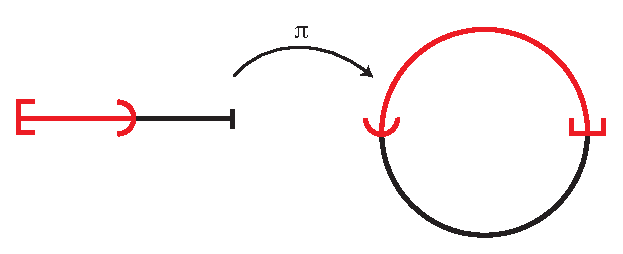
\includegraphics[width=240pt]{images/quotient_spaces/half_circle}
\end{figure}
\begin{example}
	Let $X=I \times I$, where I is the unit interval. Define an equivalence relation on X as follows: $(x,y)\sim(x',y')$ if and only if either $(x,y)=(x',y')$ or $x=x'$ and $y,y' \in \{0,1\}$. 
	
	This equivalence ``glues together'' the top and bottom edges of the unit square. This basically rolls up the unit square, so topologically $X/\sim$ gives us a cylinder.
	\[
	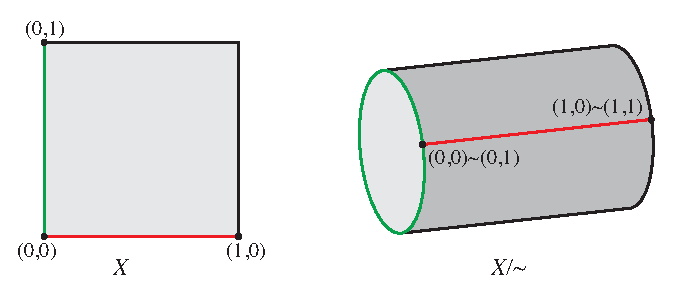
\includegraphics[width=320pt]{images/quotient_spaces/square_to_cylinder}\]
\end{example}
\begin{example}
	Let $X = \R^{2}$ and suppose $(x,y)\sim(x',y')$ if and only if $\exists n,m \in \Z$ such that $x = x' + n, y = y' + m$. 
\end{example}

Note that $X$ may be divided into integer side length squares, such that under $\sim$ all of the given squares are equivalent. Thus we need only consider one such square, noting that the opposite sides are equivalent, yielding a torus. This is pretty much the same as the above example, except that we roll up the cylinder too. In the picture, we are identifying all lines of the same color.
\[
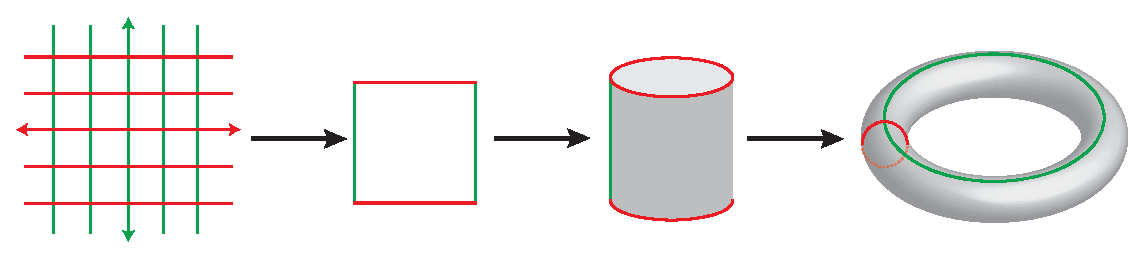
\includegraphics[width=400pt]{images/quotient_spaces/r2_torus}\]

We may also generalize this idea to higher dimensions, yielding the analogous torus for that dimension (i.e. $X = \R^{3}$ yields a 3-torus and so on). 
\begin{example}
	Let $S^{n} = \{x \in \R^{n+1}\ |\ \|x\| = 1\}.$ Define $x \sim y \Leftrightarrow x = \pm y$. 
\end{example}

Note that for $n=1$ we obtain the unit circle such that points connected by a diameter are equivalent. Thus any semi-circle forms a fundamental domain. Such a semicircle has it's endpoints as equivalent, and is thus topologically equivalent to the original circle.

We denote the quotient space $S^{n}/\sim$ by $\RP^{n}$, or the real projective space. The above argument concludes that $\RP^{1} \cong S^{1}$. 
\begin{example}
	From the above, $\RP^{2} = S^{2}/\sim$. We simply note that the fundamental domain is a hemisphere whose boundary takes on the same topology as $\RP^1$ since it is a circle under $\sim$. 
\end{example}
\begin{example}
	Let $X=\R^{2}$ and define $(x,y)\sim(x',y') \Leftrightarrow x^{2}+y^{2}=x^{'2}+y^{'2}$.
	
	Under $\sim$, any points on a circle centered at the origin are equivalent. Collapsing all such circles to points, we find that $X/\sim$ is a ray emanating from the origin (it's pink in the picture).
	\[
	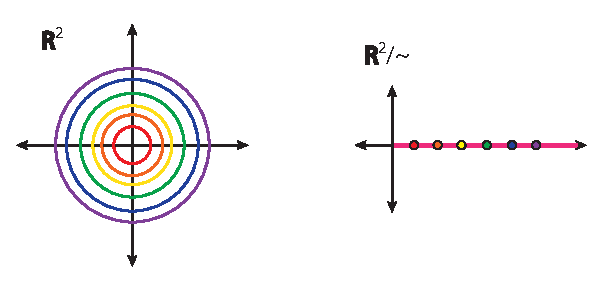
\includegraphics[width=360pt]{images/quotient_spaces/r2_ray}\]
\end{example}
\begin{definition}
	Let $X,Y$ be sets and $f: X \to Y$ be a function. We define the relation $\sim$ {\bf induced by $f$} as follows:
	
	\[\forall p,q \in X, p \sim q \Leftrightarrow f(p)=f(q)\]
	
	It is clear that $\sim$ is an equivalence relation on X because $=$ is an equivalence relation on Y. 
\end{definition}
\begin{definition}
	Suppose $(X,F_{X})$ is a topological space and Y is a set. Let $f: X \to Y$ be onto. Then the {\bf quotient topology} on Y with respect to f is given by: 
	\begin{center}
		$F_{f}=\{U \subseteq Y | f^{-1}(U) \in F_{X}\}$ 
	\end{center}
	If Y has this topology we say that f is a {\bf quotient map}. 
\end{definition}
\begin{tinyfact}
	\begin{enumerate}
		\item $(Y,F_f)$ is a topological space. 
		\item $f: (X,F_X) \rightarrow (Y,F_f)$ is continuous. 
	\end{enumerate}
\end{tinyfact}
\proof Left as an exercise. 
\begin{example}
	Let $f$ map the closed segment $[0,1]$ to a figure-eight, where $f(0)=f(1)=f(\frac{1}{2})$ at the intersection of the two sides of the figure-eight. What is open in the quotient topology $(Y,F_f)$? 
\end{example}
\begin{itemize}
	\item Any open-looking interval on the eight that does not contain the intersection point is open since its preimage is clearly open on the segment; for the same reason, any appropriate union or intersection of these open intervals is also open. 
	\item Furthermore, any open set in the figure-eight that includes the point at the cross must also contain an open interval of nonzero length extending along each of the four legs of the figure-eight. This is necessary because the definition of $F_f$ requires that the preimage of anything open must be open itself; hence the only way for the preimage of a set containing the intersection point to be open is if the preimage is an open set in $[0,1]$ containing the three preimages of the intersection point ($0$, $\frac{1}{2}$, and $1$). 
\end{itemize}

\[
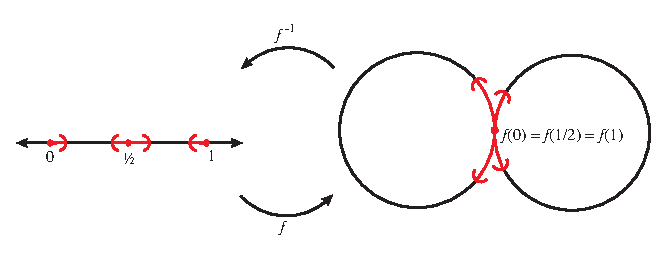
\includegraphics[width=360pt]{images/quotient_spaces/figure_eight_open_sets}\]
\begin{theorem}
	Let $(X,F_X)$ be a topological space, $f: X \twoheadrightarrow Y$ onto, and $\sim$ induced by $f$. Then $(Y,F_f) \cong (X/\sim,F_\sim)$. 
\end{theorem}

If a diagram commutes, then the path taken does not affect the result. Note that the arrow representing $g$ is dashed because we have not yet shown that the diagram commutes. In the proof, we will define $g$ so that the diagram does commute.

\[ \xymatrix{ X \ar[rr]^f \ar[ddr]^\pi & & Y \\
\\
& X/\sim \ar@{-->}[uur]^g } \]
\begin{proof}
	Define $g \colon X/\sim \rightarrow Y$ by $g([\pi]) = f(x)$ where $x$ is a representative of equivalence class $[\pi]$. We want to show that $f$ is well-defined, one-to-one, onto, continuous, and open. 
	\begin{itemize}
		\item Well-defined: WTS if $[x]=[y]$, then $g([x])=g([y])$. That is, any representative of a given equivalence class maps to the same value. Suppose $[x]=[y]$. Then $x \sim y$; since $\sim$ is the relation induced by $f$, $f(x)=f(y)$. $\therefore$ $g([x])=g([y])$. 
		\item One-to-one: Suppose $g([x])=g([y])$. Then $f(x)=f(y)$ $\Rightarrow$ $x \sim y$ $\Rightarrow$ $[x]=[y]$. 
		\item Onto: Suppose $y \in Y$. $f$ is onto, so $\exists x \in X$ such that $f(x)=y$. So $g([x]) = f(x) = y$. 
		\item Continuous: WTS $U \in F_f$ $\Rightarrow$ $g^{-1}(U) \in F_\sim$. Suppose $U \in F_f$. Recalling that $F_\sim = \{ O \subseteq X/\sim \text{ st. } \pi^{-1}(O) \in F_X \}$, we equivalently WTS that $\pi^{-1}(g^{-1}(U)) \in F_X$. Since $U \in F_f$ $\Leftrightarrow$ $f^{-1}(U) \in F_X$, we WTS $f^{-1}(U) = \pi^{-1}(g^{-1}(U))$. 
		\begin{itemize}
			\item[$(\subseteq)$] Let $x \in f^{-1}(U)$. Hence $f(x) = g([x]) \in U$. Since $\pi^{-1}(g^{-1}(U)) = \{ p \text{ st. } g \circ \pi (p) \in U \}$, $g \circ \pi (x) = g([x]) \in U$ $\Rightarrow$ $x \in \pi^{-1}(g^{-1}(U))$. 
			\item[$(\supseteq)$] Let $x \in \pi^{-1}(g^{-1}(U))$. Hence $g(\pi(x)) \in U$ $\Rightarrow$ $g([x]) \in U$ $\Rightarrow$ $f(x) \in U$. So $x \in f^{-1}(U)$. 
		\end{itemize}
		$\therefore$ $f^{-1}(U) = \pi^{-1}(g^{-1}(U))$. Since $f^{-1}(U) \in F_X$, $\pi^{-1}(g^{-1}(U)) \in F_X$. Thus $g^{-1}(U) \in F_\sim$. 
		\item Open: WTS $U \in F_\sim$ $\Rightarrow$ $g(U) \in F_f$. Suppose $U \in F_\sim$. Recalling that $F_f = \{ O \subseteq Y \text{ st. } f^{-1}(O) \in F_X \}$ and that $U \in F_\sim$ $\Leftrightarrow$ $\pi^{-1}(U) \in F_X$, we equivalently WTS $f^{-1}(g(U)) = \pi^{-1}(U)$. 
		\begin{itemize}
			\item[$(\subseteq)$] Let $x \in f^{-1}(g(U))$. So $f(x)=g([x]) \in g(U)$. Since $g$ is bijective (from the earlier parts of this proof), $[x] \in U$ $\Rightarrow$ $\pi(x) \in U$ $\Rightarrow$ $x \in \pi^{-1}(U)$. 
			\item[$(\supseteq)$] Let $x \in \pi^{-1}(U)$. So $\pi(x) \in U$, implying that $g(\pi(x)) \in g(U)$. Then $g(\pi(x)) = g([x]) = f(x)$ $\Rightarrow$ $x \in f^{-1}(g(U))$. 
		\end{itemize}
	\end{itemize}
	Therefore $g$ is a homeomorphism, and $(Y,F_f) \cong (X/\sim,F_\sim)$. 
\end{proof}
\begin{theorem}
	Let $(X,F_X)$ be a topological space and $\sim$ an equivalence relation. Let $Y = X/\sim$ and let $f : X \rightarrow Y$ be $\pi$. Then $F_\sim = F_f$ and $f$ is a quotient map. 
\end{theorem}
\begin{proof}
	Recall that: 
	\begin{align*}
		F_\sim &= \{ U \subseteq X/\sim \text{ st. } \pi^{-1} (U) \in F_x \} \\
		F_f &= \{ U \subseteq Y \text{ st. } f^{-1} (U) \in F_x \}. 
	\end{align*}
	We know that $X/\sim = Y$ and $f = \pi$. $\therefore$ $F_\sim = F_f$. Also, $f = \pi$ is onto since it is a projection, and by definition $F_\sim = F_f$ is a quotient topology. $\therefore$ $f$ is a quotient map. 
\end{proof}
\begin{lemma}
	(Important Lemma about Quotients)\\
	Let $(X,F_X)$, $(Z,F_Z)$ be topological spaces and let $Y$ be a set. Suppose $f: X \twoheadrightarrow Y$ is onto and let $g: (Y,F_f) \rightarrow (Z,F_Z)$. Then $g$ is continuous if and only if $g \circ f$ is continuous. 
\end{lemma}
\begin{proof}
	\begin{itemize}
		\item[$(\Rightarrow)$]: Suppose that $g$ is continuous. Since $f$ is a quotient map, it is continuous. Therefore, $g\circ f$ is a composition of continuous functions, and so $g\circ f$ is continuous.
		
		\item[$(\Leftarrow)$]: Suppose, now, that $g\circ f$ is continuous. Let $U\in F_Z$. Then $(g\circ f)^{-1}(U)\in F_X$. Therefore, $(g\circ f)^{-1}(U) = f^{-1}(g^{-1}(U)) \in F_X$.
		
		Recall that $F_f = \{ V\subseteq Y : f^{-1}(V)\in F_X\}$. So, $g^{-1}(U) \in F_f$, and $g$ is continuous. 
		\begin{flushright}
			$\blacksquare$ 
		\end{flushright}
	\end{itemize}
\end{proof}
\begin{example}
	(A Non-Example)\\
	Let $f: \mathbb{R}-\{1\} \rightarrow \mathbb{R}$ by
	\[ f(x) = 
	\begin{cases}
		x^2 & x\in(-\infty, 1) \\
		\frac{-1}{x-1} & x\in (1, \infty) 
	\end{cases}
	\]
	$f$ is continuous. Let $g: \mathbb{R} \rightarrow \mathbb{R}$ by
	\[ g(x) = 
	\begin{cases}
		1 & x\ge 0 \\
		-1 & x < 0 
	\end{cases}
	\]
	$g$ is not continuous. But $g \circ f: \mathbb{R}-\{1\} \rightarrow \mathbb{R}$ is defined by
	\[ (g\circ f)(x) = 
	\begin{cases}
		-1 & x > 1 \\
		1 & x < 1 
	\end{cases}
	\]
	$g \circ f$ is continuous. 
\end{example}
Question: Does this contradict the Important Lemma?

Answer: No! The solution is, of course, that $g$ actually \emph{is} continuous - the topology of its domain isn't the usual topology. Instead, it has the topology induced by $f$. That is,
\[F_f = \{ U\subseteq \R : f^{-1}(U)\text{ open in }\R\setminus\{1\} \}\]
More precisely, we have $g^{-1}(\{ 1\}) = [0, \infty)$ and $f^{-1}([0, \infty)) = (-\infty,1)$, which is open.

Also, $g^{-1}( \{-1 \} ) = (-\infty,0)$ and $f^{-1}((-\infty, 0)) = (1, \infty)$, which again is open.

Therefore, $g$ is continuous (as we only need to look at the range of $g$, which is $\{-1, 1\}$). 
\begin{theorem}
	Let $(A, F_A)$ and $(B, F_B)$ be topological spaces and $f:A\to B$ be a homeomorphism. Let $\sim_A$ and $\sim_B$ be equivalence relations on $A$ and $B$, respectively, such that $x\sim_A x'$ if and only if $f(x) \sim_B f(x')$.
	
	Then $A/\sim_A \equiv B/\sim_B$. 
\end{theorem}
\begin{proof}
	We want to show that there is some function $g$ such that the following diagram commutes:
	\[ \xymatrix{ A \ar[rr]^f \ar[dd]_{\pi_A} && B \ar[dd]^{\pi_B} \\
	&&\\C \ar @{-->}[rr]_g & & D } \]
	
	\item Define $g:A/\sim_A \to B/\sim_B$ by $g\left([x]_A\right) = \left[ f(x) \right]_B$. To show it's a homeomorphism: 
	\begin{itemize}
		\item {\bf Well-defined:} Suppose $[y]_A = [z]_A$. Then
		\[y\sim_A z\qquad\Rightarrow\qquad f(y) \sim_B f(z) \qquad\Rightarrow \qquad[f(y)]_B = [f(z)]_B]\]
		and so $g$ is well-defined. 
		\item {\bf 1-to-1:} Suppose that $[x]_A$ and $[y]_A$ are such that $g([x]_A) = g([y]_A)$. Then
		\[ [f(x)]_B = [f(y)]_B\quad\Rightarrow\quad f(x)\sim_B f(y)\quad\Rightarrow\quad x\sim_A y \quad\Rightarrow\quad [x]_A = [y]_A\]
		and so $g$ is 1-to-1. 
		\item {\bf Onto: } Let $[y]_B\in B/\sim_B$, and let $x = f^{-1}(y)$. Then
		\[ g([x]_A) = [f(x)]_B = [y]_B \]
		and $g$ is onto. 
		\item {\bf Continuous: } We want to show that $g\circ \pi_A$ is continuous, so we can use the Important Lemma. By the definition of $g$, $g\circ \pi_A = \pi_B\circ f$. Since $f$ is a homeomorphism, it is continuous; $\pi_B$ is a quotient map and is thus continuous. So $\pi_B\circ f$ is continuous. Since $g\circ \pi_A = \pi_B\circ f$, we know that $g\circ \pi_A$ is continuous. As $\pi_A$ is a quotient map, it is continuous, so from the Important Lemma, $g$ is continuous. 
		\item {\bf Open: } We can show equivalently that $g^{-1}$ is continuous instead, since $g$ is a bijection. 
		\begin{align*}
			g\circ\pi_A &= \pi_B\circ f \\
			g^{-1}\circ(g\circ\pi_A)\circ f^{-1} &= g^{-1}\circ(\pi_B\circ f)\circ f^{-1} \\
			\pi_A\circ f^{-1} & =g^{-1}\circ \pi_B 
		\end{align*}
		From here, the argument is eerily similar to the argument for continuity above.
		
		Note that $\pi_A$ is a quotient map and $f^{-1}$ s a homeomorphism, so both are continuous. As such, $\pi_A\circ f^{-1}$ is continuous, and therefore so is $g^{-1}\circ \pi_B$. Since $\pi_B$ is a quotient map, it is continuous; from the Important Lemma, $g^{-1}$ is continuous. Therefore, $g$ is open. 
	\end{itemize}
	Therefore, $g$ is a homeomorphism. Hurrah! 
\end{proof}
 


%!TEX root = ../Notes.tex
\section{The Product Topology}

For the past several pages, we've been building new topological spaces from old by using equivalence relations to form quotient spaces. Here, we will change directions and build new topological spaces from old by taking products of spaces. To that end, we wish to define the product of two sets: 
\begin{definition}
	Let $X,Y$ be sets. The product of $X$ and $Y$ is given by:
	\[X\times Y \equiv \{(x,y):\,x\in X,\,y\in Y\}\]
\end{definition}
This is a topology class, so our intrinsic urge is to find a natural topology for the product of two topological spaces. While our first instinct might be to take products of open sets in our original spaces, this approach will give unsatisfactory results: 
\begin{example}
	Consider the sets $A = (0,1)\times (0,1)$ and $B = (1/2,3/2)\times(1/2,3/2)$ as subsets of $\R\times\R = \R^2$ with the usual topology. Then $A\cup B$ in $\R^2$ is NOT a product of an open set in $\R$ with an open set in $\R$ as we would like. To intuitively see that this is not the case, see the picture! On the other hand, $A\cup B$ is open in the usual topology on $\R^2$. 
\end{example}

\[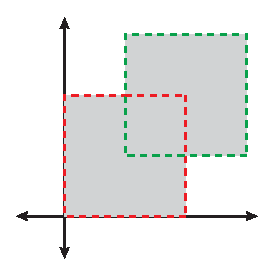
\includegraphics[width=200pt]{images/product_topology/product_sets_r}\]

Although products of open sets will not work because they are not closed under unions, we can use products of open sets to construct our topology. Define the following: 
\begin{definition}
	Let $(X,F_x)$ and $(Y,F_y)$ be topological spaces. Then the set $\beta_{X\times Y}$ is defined by:
	\[\beta_{X\times Y} = \{A\times B:\,A\in F_x,\,B\in F_y\}\]
	and define:
	\[F_{X\times Y} = \left\{\cup_{i\in I} U_i:\,I \text{ is some index set, and }U_i\in \beta_{X\times Y}\right\}\]
\end{definition}
In other words, $\beta_{X\times Y}$ is the set of products of an open set in $X$ and an open set in $Y$, and $F_{X\times Y}$ is the set of unions of elements in $\beta_{X\times Y}$. The motivation for defining our sets this way is that we want $F_{X\times Y}$ to be a topology on $X\times Y$ and for $\beta$ to be its basis. We will now verify this claim with the following \emph{small fact}: 
\begin{theorem}
	If $(X,F_x)$ and $(Y,F_y)$ are topological spaces, the space $(X\times Y,F_{X\times Y})$ is a topological space with basis $\beta_{X\times Y}$. 
\end{theorem}
\begin{proof}
	We will apply our basis theorem; i.e. we want to show that 
	\begin{enumerate}
		\item $\bigcup_{U\in \beta_{X\times Y}} U = X \times Y$ 
		\item Given $B_1,B_2\in\beta_{X\times Y}$, for each $x\in B_1\cap B_2$, there exists $B_3\in B_{X\times Y}$ such that $x\in B_3\subseteq B_1\cap B_2$. 
	\end{enumerate}
	
	For the first statement, we know that $X\in F_x$ and $Y\in F_y$ by definition of a topology so that $X\times Y\in \beta_{X\times Y}$. It follows then that because each $U\in \beta_{X\times Y}$ is subset of $X\times Y$:
	\[X \times Y \subseteq \bigcup_{U\in \beta_{X\times Y}} U \subseteq X\times Y\]
	so that $X\times Y = \bigcup_{U\in \beta_{X\times Y}} U$, as desired.
	
	For the second statement, let $B_1,B_2\in \beta_{X\times Y}$ and let $(x,y)\in B_1\cap B_2$. Then by definition of $\beta_{X\times Y}$, there exist $U_1,U_2\in F_x$ and $V_1,V_2\in F_y$ such that $B_1\cap B_2 = (U_1\times V_1)\cap (U_2\times V_2)$. 
	
	Our aim is to find $B_3\in \beta_{X\times Y}$ such that $B_3$ contains $(x,y)$ and $B_3\subseteq B_1\cap B_2$, so define:
	\[B_3 = (U_1\cap U_2) \times (V_1\cap V_2).\]
	Thus $U_1,U_2\in F_x\Rightarrow U_1\cap U_2\in F_x$ by the closure of topologies under finite intersections and similarly, $V_1\cap V_2\in F_y,$ so $B_3\in \beta_{X\times Y}$. Since $(x,y)\in (U_1 \times V_1)\cap (U_2\times V_2)$, then $(x,y)\in (U_1\times V_1)$ and $(x,y)\in (U_2\times V_2)$. Therefore, $x\in U_1,U_2$ and $y\in V_1,V_2$, so $x\in U_1\cap U_2$, and $y\in V_1\cap V_2$. It immediately follows by the definition of the intersection of sets that:
	\[(x,y) \in (U_1\cap U_2)\times (V_1\cap V_2) = B_3\]
	
	The only thing left to show is that $B_3\subseteq B_1\cap B_2$. To that end, let $(a,b)\in B_3$. Then $a\in U_1\cap U_2$ and $b\in V_1\cap V_2$ by definition of $B_3$. It follows that:
	\[a\in U_1,U_2 \text{ and } b\in V_1,V_2 \Rightarrow (a,b)\in U_1\times V_1 \text{ and } (a,b)\in U_2 \times V_2 \Rightarrow a\in (U_1\times V_1)\cap (U_2\times V_2).\]
	Therefore, $(a,b)\in B_1\cap B_2$ so that $B_3\subseteq B_1\cap B_2$ because $(a,b)$ is an arbitrary element of $B_3$. 
	
	Therefore, $\beta_{X\times Y}$ satisfies the hypotheses of our basis theorem, so the set of unions of elements of $\beta_{X\times Y}$, $F_{X\times Y}$, is a topology for $X\times Y$ and $\beta_{X\times Y}$ is a basis for the topology $F_{X\times Y}$. 
\end{proof}

We have successfully devised a topology for product spaces as unions of products of open sets.

\subsection{Examples}
\begin{example}
	The set $S^1 \times [0,1]$ looks like a cylinder! What kinds of sets are open in the cylinder? A particular example is an open disc projected on the face of the cylinder and unions thereof. 
\end{example}
\[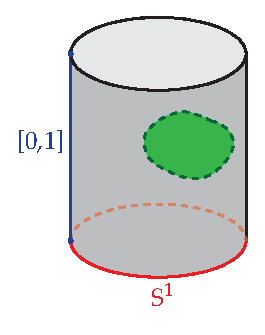
\includegraphics[width=100pt]{images/product_topology/s1_times_i}\]

\begin{example}
	The set $S^1 \times S^1$ looks like a torus! What kinds of sets are open in the torus? Similar to the previous example, open discs projected onto the torus surface are examples of open sets in $S^1\times S^1$.  In the picture, one copy of $S^1$ is red and one is green; they determine a torus.
\end{example}

\[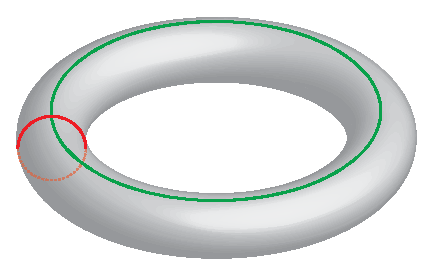
\includegraphics[width=160pt]{images/product_topology/s1_times_s1}\]

\begin{example}
	The set $S^1 \times S^1 \times S^1$ is actually a 3-torus! 
\end{example}

Not every space is a product of more than one space. For example the sphere $S^2$ is not a product of more than one space. An intuitive (non-rigorous) justification is that the natural axes of a sphere are the great circles; however, every pair of distinct great circles intersect twice which makes it hard to define a coordinate system on the sphere.

\subsection{The Product Projection Map}

Now that we have a product topology to impose on product spaces, we want a way to relate the product topology to the topologies of the constituent spaces. In order to do so, we will define the projection maps as follows: 
\begin{definition}
	Let $(X,F_x)$ and $(Y,F_y)$ be topological spaces and create $X\times Y$ endowed with the product topology $F_{X\times Y}$. Define $\pi_X: (X\times Y,F_{X\times Y}) \to (X,F_x)$ and $\pi_Y:(X\times Y,F_{X\times Y}) \to (Y,F_y)$ by:
	\[\pi_X((x,y)) = x \qquad \pi_Y((x,y)) = y.\]
	The map $\pi_X$ is the projection onto $X$ and $\pi_Y$ is the projection onto $Y$. 
\end{definition}

A small fact which we will derive now is that the product projection maps are continuous: 
\begin{theorem}
	Let $(X,F_X)$ and $(Y,F_Y)$ be topological spaces and $(X\times Y,F_{X\times Y})$ be their product with the induced product topology. Then the projection maps $\pi_X$ and $\pi_Y$ onto $X$ and $Y$ are continuous. 
\end{theorem}
\begin{proof}
	Suppose $O\subseteq X$ and $O\in F_x$. We see that $\pi^{-1}(O) = O\times Y \in F_{X\times Y}$. Therefore, the preimage of any open set in $X$ under $\pi_X$ is open in $X\times Y$ with the product topology. A similar argument shows that $\pi_Y$ is continuous. 
\end{proof}

Recall that the quotient projection map is \emph{not necessarily} an open map. It turns out that the product projection map \emph{is} an open map. Accidentally assuming that the quotient map is open is a very common mistake that one should be aware of! We will now prove that the product projection map is open: 
\begin{theorem}
	Let $(X,F_X)$ and $(Y,F_Y)$ be topological spaces and $(X\times Y,F_{X\times Y})$ be their product with the induced product topology. Then the projection maps $\pi_X$ and $\pi_Y$ onto $X$ and $Y$ are open. 
\end{theorem}
\begin{proof}
	Let $O = U\times V$ such that $U \in F_x$ and $V\in F_y$ and $O\in \beta_{X\times Y}$. Therefore:
	\[\pi_X(O) = U\in F_x\]
	So if $C$ is some collection of sets in $\beta_{X\times Y}$, then:
	\[\bigcup_{V\in C}V\]
	is an arbitrary element of $F_{X\times Y}$ by the definition of a basis and:
	\[\pi_X\left( \bigcup_{V\in C}V \right) = \bigcup_{V\in C} \pi_X(V)\]
	which is open because the preceding statments indicate that $V\in \beta_{X\times Y} \Rightarrow \pi_X(V)\in F_X$. Consequently, the image of the arbitrary open set in $(X\times Y, F_{X\times Y})$ is a union of open sets in $(X,F_x)$ and is thus open.
	
	The proof is similar for $\pi_Y$. 
\end{proof}

\subsection{Using Bases More Effectively}

In metric spaces, open balls are bases for the metric topology. By proving properties about open balls, we were able to say they apply to the entire set. We would like to prove the following \emph{important tiny lemma} so that we can use bases in topological spaces like open balls in metric spaces: 
\begin{lemma}
	Let $(X,F_x)$ be a topological space with basis $\beta$. If $W\subseteq X$ then $W\in F_x$ if and only if for all $p\in W,$ there exists $B_p\in\beta$ such that $p\in B_p\subseteq W$. 
\end{lemma}
\begin{proof}
	\begin{itemize}
		\item[$(\Rightarrow)$] Suppose $W\in F_x$. Let $p\in W$. Since $W\in F_x$, for some index set $I$:
		\[W = \bigcup_{i\in I}B_i \qquad \forall i\in I,\,B_i\in \beta\]
		because every element of a topology can be written as a union of basis elements. Therefore, by definition of the union, $p\in W$ implies that there exists $i_p\in I$ such that $p\in B_{i_p}$, and $B_{i_p}\subseteq W$. If we let $B_p = B_{i_p}$, we are finished.
		
		\item[$(\Leftarrow)$]
		
		Suppose that for all $p\in W$, there exists $B_p\in \beta$ such that $p\in B_p\subseteq W$. We want to show that $W\in F_x$. We see that:
		\[V = \bigcup_{p\in W}B_p\subseteq W\]
		because each of the constituent $B_p\subseteq W$, and every $p\in W$ is an element of $B_p$, so the union of $B_p$ over $p\in W$, contains every $p\in W$. Consequently, $V\subseteq W \Rightarrow V=W$. Since $\beta$ is a basis and $V$ is a union of basis elements, $V\in F_x \Rightarrow W\in F_x$. 
	\end{itemize}
\end{proof}

In other words, if we have a topological space with a basis, then every point in an open set $U$ is an element of a basis element contained in $U$, giving us a structure very similar to the metric topology.

\subsection{Finding and Constructing Continuous Maps to Product Spaces}

Now that we have product spaces and have addressed their basic topological properties, we would like a way to easily find and construct continuous maps to the product space. To that end we introduce the following \emph{important lemma}: 
\begin{lemma}
	Let $(X,F_X),(Y,F_Y)$ and $(A,F_A)$ be topological space and let $(X\times Y,F_{X\times Y})$ be the product space of $X,Y$ with the induced product topology. Suppose $f:A\to X$ and $g:A\to Y$ and define
	\[h:A\to(X\times Y) \qquad \text{ by } \qquad h(a) = (f(a),g(a)),\]
	then $h$ is continuous if and only if $f,g$ are continuous. 
\end{lemma}
\begin{proof}
	\begin{itemize}
		\item[$(\Rightarrow)$] Suppose $h$ is continuous: then we see that:
		\[f = \pi_X \circ h \qquad g = \pi_Y \circ h\]
		so $f,g$ are continuous because they are compositions of continuous functions. 
		\item[$(\Leftarrow)$] Suppose that $f$ and $g$ are continuous. We prove that the preimage of every basis element under $h$ is open. From a theorem we proved some time ago, this shows that $h$ is continuous.
		
		Let $U\times V\in \beta_{X\times Y}$. Then $U\in F_X$ and $V\in F_Y$. Since $f$ and $g$ are continuous, $f^{-1}(U)\in F_A$ and $g^{-1}(V)\in F_A$. Then 
		\begin{align*}
			h^{-1}(U\times V) &= \{a\in A\ |\ h(a)\in U\times V\}\\
			&= \{a\in A\ |\ (f(a), g(a))\in U\times V\}\\
			&= \{a\in A\ |\ f(a)\in U, g(a)\in V\}\\
			&= f^{-1}(U)\cap g^{-1}(V) 
		\end{align*}
		Then $h^{-1}(U\times V)$ is the intersection of two open sets, hence it is open. Therefore, $h$ is continuous. 
	\end{itemize}
\end{proof}

The following example illustrates how this lemma makes it very easy to define continuous functions to the product space: 
\begin{example}
	Suppose $f:\R\to\R$ and $g:\R\to\R$ with $f(x) = x^2+3x$ and $g(x) = \sin(x)$. Then the map $h:\R\to\R^2$ defined by $h(x) = (x^2+3x, \sin(x))$ is continuous because $f,g$ are. 
\end{example}

\subsection{Relating Products to Subspaces} 
\begin{smallfact}
	Let $(X, F_X)$ and $(Y, F_Y)$ be topological spaces with subspaces $(A, F_A)$ and $(B, F_B)$ respectively. Let $F_S$ denote the subspace topology on $A\times B\subseteq X\times Y$ and let $F_{A\times B}$ denote the product topology on $A\times B$. Then $F_S = F_{A\times B}$. 
\end{smallfact}
This means that we can either look at $A\times B$ as a subspace of $X\times Y$, then induce the subspace topology, or we can induce the subspace topologies on $A$ and $B$, then take the cross product. Essentially, taking the cross product and creating subspaces ``commute.'' 
\begin{proof}
	We start by reviewing which sets are open under each topology:
	\[ F_S = \{ (A\times B)\cap U\ |\ U\in F_{X\times Y} \}\]
	\[ F_{X\times Y} = \text{unions of sets of the form } U\times V\text{, with } U\in F_A, V\in F_B \]
	
	Let $U\cap(A\times B)\in F_S$. Then
	\[ U\cap(A\times B) = \bigcup_{i\in I} (U_i\times V_i)\cap (A\times B) \qquad\qquad\text{(where }\forall i\in I, U_i\in F_X, V_i\in F_Y)\]
	Then 
	\begin{align*}
		U\cap(A\times B) &= \bigcup_{i\in I} (U_i\times V_i)\cap (A\times B)\\
		&= \{ (x,y)\in A\times B\ |\ (x,y)\in U_{i'}\times V_{i'}\text{ for some }i'\in I \} \\
		&= \{ (x,y)\in X\times Y\ |\ x\in U_{i'}\cap A, y\in V_{i'}\cap B\text{ for some }i'\in I\} \\
		&= \bigcup_{j\in J} (U_j\cap A)\times (V_j\cap B)\qquad\qquad\text{ for some index set} J \}\\
		&\in F_{X\times Y} 
	\end{align*}
	The same argument run backwards shows that $F_{X\times Y}\subseteq F_S$.
	
	Therefore, $F_{S} = F_{X\times Y}$. 
\end{proof}

\subsection{Products and Quotient Spaces} Taking products and quotients does not ``commute'' in the same way that taking products and subspaces does. We demonstrate a (lengthy) counterexample to this idea.

Consider $\R$ with the usual topology, with $x\sim Y$ iff $x=y$ or $x,y\in \N$. This looks something like a ``sideways infinite flower.'' 

\[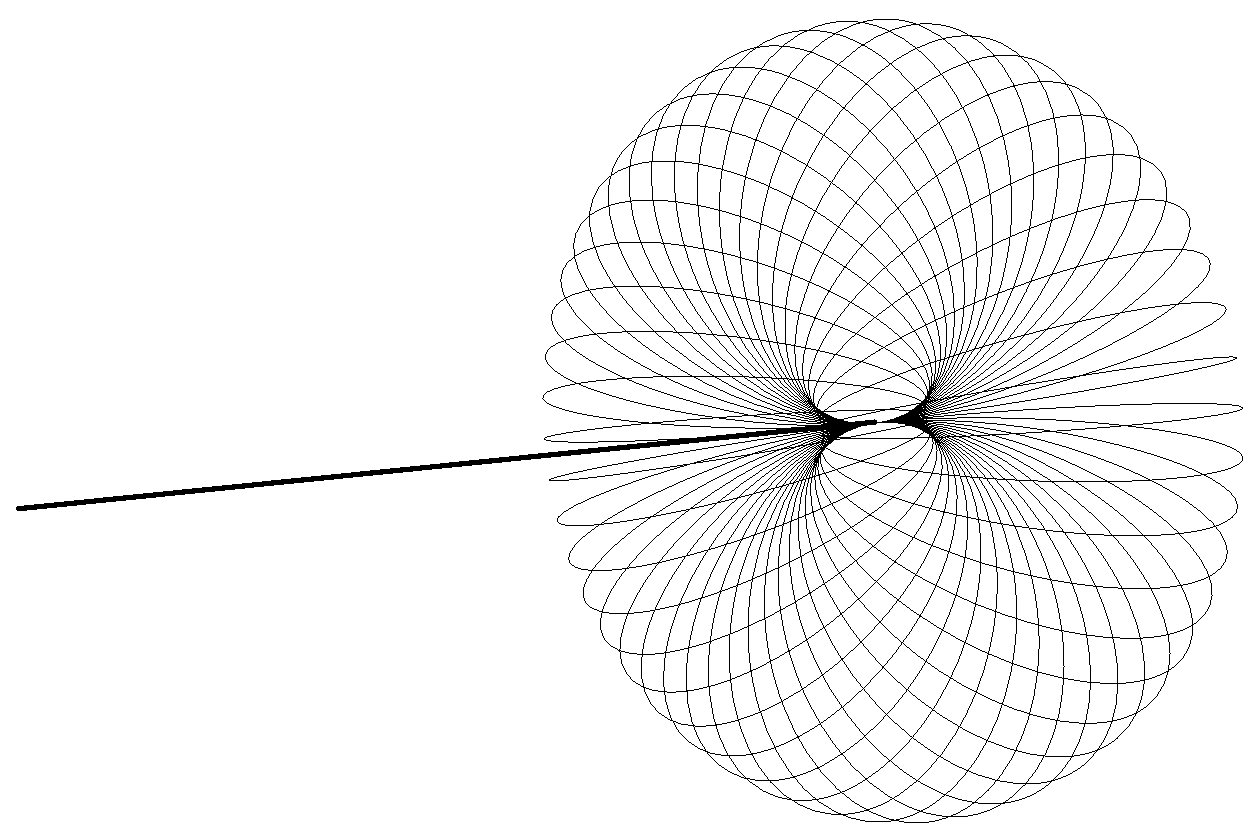
\includegraphics[width=200pt]{images/product_topology/sideways_infinite_flower}\]

 If a set open in $\R/\sim$ contains a (``the'') natural number, then its preimage must contain every natural number, so it must contain an open interval about ``the'' natural number in every direction (all infinity of them). 

More formally, let $\pi:\R\to\R/\sim$ be the projection map. Let $id_\Q:\Q\to\Q$ be the identity map, where each copy of $\Q$ has the usual topology. Note that $id_\Q$ is a quotient map (where $\sim$ is `='). 

Now, consider $\pi\times id_\Q:\R\to\Q\to(\R/\sim)\times\Q$ by $(\pi\times id_\Q)(x,y) = (\pi(x), i(y))$. We claim that $\pi\times id_\Q$ is not a quotient map. To prove this, we show that the product topology on $(\R/\sim)\times\Q$ is not the same as the quotient topology
\[ \{ U\in (\R/\sim)\times\Q\ |\ (\pi\times id_\Q)(U)\in F_{\R\times\Q} \} \]
To do this, let's find some $U' \in F_{\pi \times i}$ such that $U' \notin F_{(\R/\sim) \times \Q}$. We want to construct $U'$ as a union.

For all $n\in \N$ define $U_n$ to be the interior of the region of $\R\times\Q$ bounded by the vertical lines $n-\frac{1}{4}$ and $n+\frac{1}{4}$ and above and below by the lines through $(n, \frac{\sqrt{2}}{n})$ with slope $\pm 1$. Each one of these sets has a vertical line through the natural number.

So $\forall n \in \N, \{n\}\times \Q \subseteq U_n$. Observe that $\forall n\in \N, U_n \in F_{\R\times\Q}$ (it is an interior, so it is open).

Let $\bigcup_{n \in\N} U_n \in F_{\R\times\Q} \qquad$ (also open in $\R\times\Q$ because it is a union).

Let $U' = (\pi \times i)(U).$ This will glue together the strips along the vertical lines with $\R$ coordinates in $\N$. This can be pictured as a fan.
\[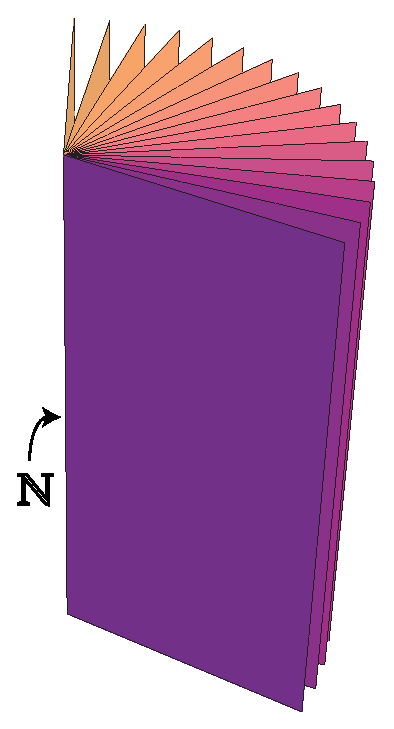
\includegraphics[width=100pt]{images/product_topology/sideways_infinite_fan}\]

Claim: $U' \in F_{\pi \times i}$

\proof: $(\pi \times i)^{-1}(U') = U$ and $U$ is a union of $U_n 's$

Therefore, by definition, $U'\in F_{\pi\times i}$.

\mbox{ }

Claim: $U'\not\in F_{(\R/\sim) \times \Q}$.

\proof: Let $([n],0) \in U'$. Suppose $\exists W \in F_{\R/\sim}$ and $V \in F_{\Q}$ such that $([n], 0)\in W \times V \subseteq U'$.

Then $\pi^{-1}(W) \in F_{\R}$ and of course $i^{-1}(V) = V$.

So $\pi^{-1}(W) \times V$ is open in $\R\times \Q$ such that $\pi^{-1}(W) \times V \subseteq (\pi \times i)^{-1}(U') = U$.

Also, $\pi^{-1}(W)$ is open in $\R$ and contains $\N$ and $V$ is open in $\Q$ and contains $\{0\}$.

So $\exists \delta >0$ such that $(-\delta, \delta) \cap \Q \subseteq V$. There exists an $n\in \N$ such that $\delta > \frac{\sqrt{2}}{n}$. $\pi^{-1}(W)$ is open in $\R$, so it's on the x-axis.

So $\exists \epsilon >0$ such that $(n-\epsilon, n+\epsilon)\subseteq \pi^{-1}(W)$.

So the interval $(n-\epsilon, n+\epsilon)\times (-\delta, \delta)\subseteq \pi^{-1}(W)\times V$. So $\epsilon < \frac{1}{4}$ from our previous definition of $U_n$.

Let $x = n + \frac{\epsilon}{2}$. Question: Where does $x = n + \frac{\epsilon}{2}$ meet the boundaries of $U_n$? It meets at $y = \frac{\sqrt{2}}{n} \pm \frac{\epsilon}{2}$.

$\exists y \in \Q$ such that $\frac{\sqrt{2}}{n} - \frac{\epsilon}{2} < y < \frac{\sqrt{2}}{n} + \frac{\epsilon}{2}$.

So $(x,y) \notin U_n$ and $\forall m\neq n, (x,y)\notin U_m$ since $(x,y) \in (n-\epsilon, n+\epsilon)\subseteq (n-\frac{1}{4}, n+\frac{1}{4}$.

But $(x,y) \in (n-\epsilon, n+\epsilon) \times (-\delta, \delta) \subseteq \pi^{-1}(W) \times V \subseteq U$ $\Rightarrow (x,y) \notin U$. Therefore we have a contradiction.

$\therefore U' \notin F_{(\R/\sim)\times \Q}$

So we have shown that $F_{\pi\times i} \neq F_{(\R/\sim) \times \Q}$.

\subsection{Infinite Products} We would of course like to be able to generalize this to deal with infinite products. Initially, we may simply want to define such products as follows: $X_1$x$X_2$x...$=\{(x_1,x_2,...)|x_i \in X_i \forall i \in \N \}$. However, such a definition limits us to countable products, so we look more generally.
\begin{definition}
	$j \in J$, let $X_j$ be a set. Define the product $\Pi_{j \in J} X_j = \{f:J \rightarrow \cup_{j \in J}X_j|f(j) \in X_j\}.$ We refer to $f(j)$ as the $j^{th}$ coordinate of the point $f$. 
\end{definition}
\begin{example}
	Suppose $J = \{1,2\}$. Then $\Pi_{j\in \{1,2\}}X_j = \{f: \{1,2\} \rightarrow X_1\cup X_2|f(j) \in X_j\} = \{(f(1),f(2))|f(j) \in X_j\}=\{(x_1,x_2)|x_j \in X_j\} = X_1$ x $X_2.$ Thus we see that this definition agrees with our previous definition for finite products. 
\end{example}
\begin{example}
	Consider $\Pi_{j \in \R}\{1,2\}$. By definition this is equivalent to $\{f: \R \rightarrow \{1,2\}| f(j) \in \{1,2\}, j \in \R\}$, which precisely correspond to subsets of $\R$ if we simply think of the preimage of $1$ under $f$ as the elements in the set and the preimage of $2$ under $f$ as those elements outside the set. Commonly this product is then denoted by $\{1,2\}^{\R}$. 
\end{example}

Now we wish to define a topology on these products which, as in example $1$, agrees with our prior definition for a product of two sets if the indexing set $J = \{1,2\}$. Perhaps the most natural way of doing this is to define the following basis: 
\begin{center}
	$\beta_{\Box} = \{\Pi_{j \in J} U_j|U_j \in F_j\}$, where $X_j$ has topology $F_j$.
	
	$F_{\Box} = \{$Unions of elements of $\beta_{\Box}\}.$ 
\end{center}
This topology is not what we desire, but is a topology, aptly named the box topology on the product.
\begin{example}
	The product topology on $\Pi_{j \in J}X_j$ is given by the basis $\beta_{\Pi} = \{\Pi_{j \in J}U_j|U_j = X_j$ for all but finitely many $j$ and $\forall j \in J, U_j \in F_j \}$. 
\end{example}

Remarks: 
\begin{enumerate}
	\item $\beta_{\Pi} \subseteq \beta_{\Box}$ 
	\item Both are bases for topologies on the product. 
\end{enumerate}
\begin{definition}
	Define the projection map $\pi_j : \Pi_{j \in J}X_j \rightarrow X_j$ by $\pi(f) = f(j)$. 
\end{definition}
\begin{lemma}
	For all $j \in J$, Suppose $(X_j, F_j)$ is a topological space. Then $\pi_j$ as defined above is continuous for all $j \in J$. 
\end{lemma}
\begin{proof}
	Let $j_{0} \in J$ and consider $U \in F_{j_{0}}$. We wish to show that $\pi_{j_{0}}^{-1}(U) \in F_{\Pi}$. Note that $\pi_{j_{0}}^{-1}(U) = \{f \in \Pi_{j \in J}X_j | \pi_{j_{0}}(f) \in U\} = \{f \in \Pi_{j \in J}X_j | f(j_{0}) \in U\} = \{f \in \Pi_{j \in J}X_j | f(j_{0}) \in U, \forall j \neq j_{0} f(j) \in X_{j}\}= \Pi_{j \in J} U_j$ such that $U_{j_{0}} = U$ and $\forall j \neq j_{0}, U_j = X_j$.\\
	It then follows from definitions that $\pi_{j_{0}}^{-1}(U) \in \beta_{\Pi} \subseteq F_{\Pi}$ so the projection map is continuous. 
\end{proof}

We now prove an Important Lemma for Infinite Products. 
\begin{lemma}
	Let $(X_j,F_j)$ and $(Y,F_Y)$ be topological spaces for all $j \in J$. Moreover, for each such j let $g_j : Y \rightarrow X_j$ be a function. Define $h: Y \rightarrow \Pi_{j \in J}X_j$ by: $h(y) = f$ such that $\forall j \in J, f(j) = g_{j}(y)$. Then $h$ is continuous if and only if $g_j$ is continuous for all $j \in J$. 
\end{lemma}
\begin{proof}
	\begin{itemize}
		\item[($\Rightarrow$)] Suppose $h$ is continuous and let $j \in J$. Then $\pi_j \circ h = g_j$. Thus $g_j$ is the composition of continuous functions and must itself be continuous. 
		\item [($\Leftarrow$)] Suppose that $g_j$ is continuous for all $j \in J$. Let $U \in \beta_{\Pi}.$ We wish to show that $h^{-1}(U) \in F_{Y}$.
		
		Note that $h^{-1}(U) = \{y \in Y | h(x) \in U\}$ As an open set in the product topology, $U = \Pi_{j \in J}U_j$ where $U_j \in F_j$. Thus, $h^{-1}(U) = \{y \in Y | h(x) \in \Pi_{j \in J}U_j\} = \{f \in \Pi_{j \in J}U_j$ such that $\forall j \in J, f(j) = g_{j}(y)\} = \{y \in Y | g_{j}(y) \in U_j\} = \{y \in Y | y \in g_{j}^{-1}(U_j) \forall j \in J\} = \cap_{j \in J} U_j$.
		
		Since $g_j$ is continuous for all $j$, $g_{j}^{-1}(U_j)$ is open in $Y$ for all $j$. Also, by definition of the product topology, $U_j = X_j$ for all but at most finitely many $j$. Thus, $g_{j}^{-1}(U_j) = Y$ for all but at most finitely many $j$. It follows that the intersection $\cap_{j \in J} U_j$ is a finite intersection of open sets since removing all trivial indices will not change the intersection. Thus, $h^{-1}(U) \in F_Y$ so $h$ is continuous, completing the proof. 
	\end{itemize}
\end{proof}
 


%!TEX root = ../Notes.tex
\chapter{Distinguishing Spaces} 
\begin{definition}
	A {\bf topological property} (or `top. prop.') is a property of a topological spaces that is preserved by homeomorphisms. 
\end{definition}
\begin{center}
	{\bf List of Topological Properties thus Far} 
\end{center}
\begin{enumerate}
	\item Cardinality of $X$ 
	\item Cardinality of $F_x$ 
	\item Metrizability (we proved this in the homework) 
	\item Discreteness 
	\item Indiscreteness 
\end{enumerate}
\begin{lemma}
	{\bf (Rachel's Lemma)}\\
	Let $(X, F_X) $ and $(Y, F_Y)$ be topological spaces and $f: X \rightarrow Y$ be an open bijection. If $F_X$ is the discrete topology, then $F_Y$ is the discrete topology. 
\end{lemma}
\begin{proof}
	Let $y \in Y$. Since $f$ is surjective, there exists $x \in X$ such that $f(x) = y$. Since $\{x\} \in F_X$ and $f$ open, $f(\{x\}) \in F_Y$. Thus all singletons in are elements of $F_Y$ and all sets in $Y$ are unions of singletons and hence elements of $F_Y$, so every set is an open set and $F_Y$ is the discrete topology. 
\end{proof}
\begin{lemma}
	{\bf (Daniel's Lemma)}\\
	Let $(X, F_X) $ and $(Y, F_Y)$ be topological spaces and $f: X \rightarrow Y$ be a continuous bijection. If $F_X$ is the indiscrete topology, then $F_Y$ is the indiscrete topology. 
\end{lemma}
\begin{proof}
	Let $U \in F_Y$. WTS $U = Y$ or $U = \emptyset$. Since $f$ is continuous, $f^{-1}(U) \in F_X$. Therefore $f^{-1}(U) = X$ or $\emptyset$. \\
	Suppose $f^{-1}(U) = X$. Then $U = f(f^{-1}(U)) = f(X) = Y$ since $f$ surjective.\\
	Suppose $f^{-1}(U) = \emptyset$. Then $U = \emptyset$. Therefore $F_Y$ is the indiscrete topology. 
\end{proof}

{\bf Corollaries} If $(X, F_X) $ and $(Y, F_Y)$ topological spaces and $f: X \rightarrow Y$ a homeomorphism, then 
\begin{enumerate}
	\item $F_X$ the discrete topology $\Longrightarrow$ $F_Y$ the discrete topology 
	\item $F_X$ the indiscrete topology $\Longrightarrow$ $F_Y$ the indiscrete topology 
\end{enumerate}

Unfortunately, even with these five lovely Topological Properties, we can't yet distinguish a circle from a line. Clearly there is more work to do.
\begin{example}[a non-example]
	Distance is not a topological property. A big circle \emph{is} homeomorphic to a little circle. 
\end{example}

\section{Compactness}
\begin{definition}
	Let $(X, F_X)$ be a topological space and $S \subseteq X$.\\
	We say $\{U_j : j \in J\}$ is an $\mathbf{open \ cover}$ of $S$ if for all $j \in J$, $U_j \in F_X$ and $S \subseteq \bigcup_{j \in J}U_j$.\\
	We say $\{U_j : j \in K\}$ is a {\bf subcover} if $K \subseteq J$ and $S \subseteq \bigcup_{j \in K} U_j$.
	
	We say $S$ is {\bf compact} if every open cover of $S$ has a finite subcover. 
\end{definition}

{\bf IMPORTANT WARNING!}\\
We learned in Math 131 that in $\R^{n}$, a set if compact $\Longleftrightarrow$ it is closed and bounded. THIS IS NOT TRUE IN TOPOLOGICAL SPACES. DO NOT TRY TO USE IT.
\begin{example}
	Is the set $(0,1)$ compact in 
	\begin{enumerate}
		\item $\R$ with the discrete topology? 
		\item $\R$ with the half-open topology? 
		\item $\R$ with the finite complement topology? 
	\end{enumerate}
\end{example}

Answers: 
\begin{enumerate}
	\item No. Take the open covering $\{B_{1/2}(x) : x \in (0,1)\}$. If we remove any of these balls, the corresponding $x$ will no longer be covered. However, there are clearly uncountably infinitely many balls. \\\\
	\item No. Take the open covering $\{[\frac{1}{n}, 1) : n \in \N\}$ so that $(0,1) = \bigcup_{n \in \N}([\frac{1}{n}, 1)$. There is not finite subcover. \\\\
	\item Yes. Suppose we have a cover of $(0,1)$. Take any element of the cover, say $U_{47}$. $U_{47}$ is missing at most finitely may elements of $(0,1)$ since its complement is finite. For each element $x \in \R \setminus U_{47}$, select one $U_{j_x}$ containing $x$. The set $\{U_{47}\} \cup \{U_{j_x}: x \in \R \setminus U_{47}\}$ is a finite open subcover. 
\end{enumerate}
\begin{theorem}
	(analogous to a theorem from 131)\\
	Let $(X, F_X)$ and $(Y, F_Y)$ be topological spaces, $S \subseteq X$, and $f : X \rightarrow Y$ continuous. If $S$ is compact then $f(S)$ is compact. 
\end{theorem}
\begin{proof}
	\begin{enumerate}
		\item Take a covering of $f(S)$. 
		\item Applying $f^{-1}$ to these sets, we pull back to an open covering of $S$. 
		\item Take a finite subcover. 
		\item Push these forward again. We have a finite cover of $f(S)$. 
	\end{enumerate}
\end{proof}

As a corollary we have {\bf Topological Property 6: Compactness}.\\
\begin{theorem}
	Any closed subset of a compact space is compact. 
\end{theorem}
\begin{proof}
	\begin{enumerate}
		\item Take an open cover of $S$ 
		\item Add $X \setminus S$. Now we have an open cover of $X$. 
		\item Take a finite subcover. 
		\item Remove $X \setminus S$. Not we have a finite subcover of $S$. 
	\end{enumerate}
\end{proof}
\begin{theorem}
	(also analagous to a 131 theorem)\\
	Let $(X, F_X)$ be compact and $f : X \rightarrow \R$ be continuous. Then $f$ has a max value and a min value. 
\end{theorem}
\begin{proof}
	\begin{enumerate}
		\item $f(X)$ is compact by Analogous Theorem 1 
		\item Therefore $f(X)$ is closed and bounded 
		\item Therefore $f(X)$ has a lub and a glb (ie a max and a min) 
	\end{enumerate}
\end{proof}
\begin{smallfact}
	Let $(X, F_X)$ be a topological space. Suppose every open cover of $S \subseteq X$ made up of basis elements has a finite subcover. Then $X$ is compact. 
\end{smallfact}
\begin{proof}
	Let $\{U_j : j \in J\}$ be an open cover of $S$ and $\beta$ be a basis of $S$. For every $j \in J$, $U_j = \bigcup_{i \in I_j}B_i$ where for every $i \in I_j$ $B_i \in \beta$. Hence $\{B_i : i \in I_j \text{ and } j \in J\}$ is an open cover of $S$. By hypothesis, we have a finite subcover, $\{B_i : i \in K_j \text{ and } j \in K\}$ where $K \subseteq J$ and $K$ is finite, and for all $j \in K$, $K_j \subseteq I_j$ and $K_j$ is finite. Now note that given any $j \in K$, for every $i \in K_j$ $B_i \subseteq U_j$. Hence
	\[X = \bigcup_{j\in K} \left[ \bigcup_{i \in K_j} B_i \right] \subseteq \bigcup_{j\in K} U_j \subseteq X\]
	and $\{U_j : j\in K\}$ is a finite subcover. 
\end{proof}
\begin{theorem}
	(Bolzanno-Weierstrass Theorem).\\
	Let $(X,F_X)$ be a compact topological space. Then for all infinite $S \subseteq X$, $\exists \ p \in X$ such that $\forall \ U \in F_X$ with $p \in U$, $U$ contains infinitely many points of $S$. 
\end{theorem}
\begin{proof}
	Suppose that for some such $S \subseteq X$, no such $p \in X$ exists. Therefore, for all $p \in X$ there exists some $U_p \in F_X$ such that $p \in U_p$ and $|S \cap U_p|$ is finite. So, as $\displaystyle{\bigcup_{p \in X} U_p = X}$, $\{U_p \mid p \in X\}$ is an open cover of $X$. As $X$ is compact, there exists some finite subcover $\{U_{p_1},...,U_{p_n}\}$. Hence, from the definition of a subcover, $\displaystyle{X = \bigcup_{i=1}^n U_{p_i}}$. Intersecting both sides with $S$ gives that:
	\[S = \left(\bigcup_{i=1}^n U_{p_i}\right) \cap S = \bigcup_{i=1}^n (U_{p_i} \cap S)\]
	However, as $|U_p \cap S|$ is finite for all $p \in X$, $|U_{p_i} \cap S|$ is finite for $1 \leq i \leq n$. The union of finite sets is finite, and therefore $\left|\bigcup_{i=1}^n (U_{p_i} \cap S)\right|$ is finite. However, $S$ is infinite by assumption. So this is a contradiction, and no such $S$ exists. 
\end{proof}
\newpage
\begin{theorem}
	(Finite Tychonoff Theorem) \\
	Let $(X,F_X)$ and $(Y,F_Y)$ be compact topological spaces. Then $(X \times Y, F_{X \times Y})$ is also a compact topological space. 
\end{theorem}
\begin{proof}{Comic book style}  \mbox{ }\\
	
	\begin{figure}[h!]
		\begin{center}
		\subfigure[Consider some open cover.]{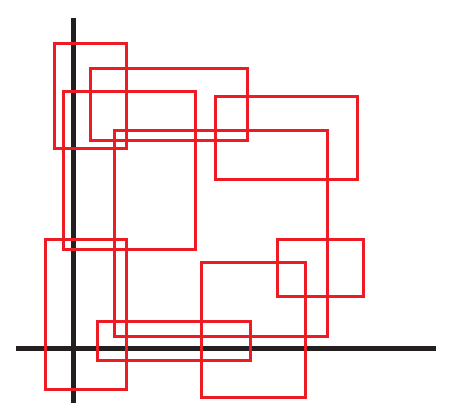
\includegraphics[width=180pt]{images/compactness/tychonoff_comic_1}}
		\subfigure[Restrict to some $\{x\} \times Y$, which is compact, so has a finite subcover.]{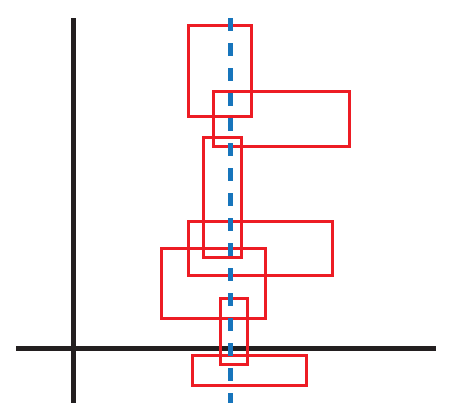
\includegraphics[width=180pt]{images/compactness/tychonoff_comic_2}}
		\end{center}
		\begin{center}
		\subfigure[So there is some open $U_x$ with $x \in U_x$ s.t. $U_x \times Y$ is contained in this subcover.]{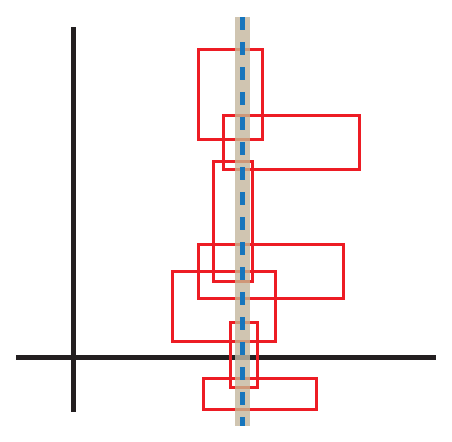
\includegraphics[width=180pt]{images/compactness/tychonoff_comic_3}}
		\subfigure[So consider just the $U_x$, which are a cover of $X$, so have a finite subcover.]{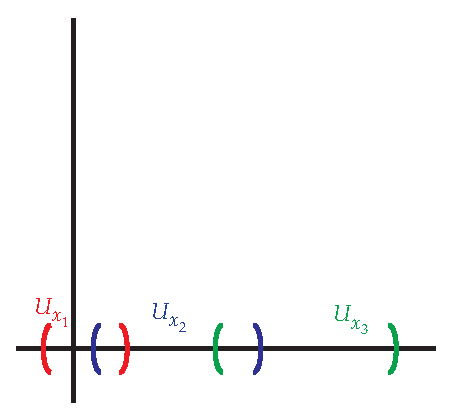
\includegraphics[width=180pt]{images/compactness/tychonoff_comic_4}}
		\end{center}
	\end{figure}
	
	So the original sets that covered $\{x\} \times Y$ corresponding to the chosen $U_x$ for the desired finite cover of $X \times Y$. 
\end{proof}
Now let's do a real proof. 
\begin{proof}{Real}
	Consider an open cover of $X \times Y$ consisting of basis elements, $\{U_i \times V_i \mid i \in I\}$, where $U_i \in F_X$ and $V_i \in F_Y$ for all $i \in I$.
	
	Let $x \in X$. It is clear that $\{x\} \times Y \cong Y$, so $\{x\} \times Y$ is compact. So the original open cover is a cover of $\{x\} \times Y$, and there exists some finite subcover $\{U_{i(x)} \times V_{i(x)} \mid i(x) \in K_x\}$ where $K_x \subseteq I$ and $K_x$ is finite. If $x \notin U_{i(x)}$, removing the set $U_{i(x)} \times V_{i(x)}$ does not change the fact that the remaining set is a finite subcover of $\{x\} \times Y$. Hence, without loss of generality, we assume that $x \in U_{i(x)}$ for all $i(x) \in K_x$.
	
	Next, define $\displaystyle{U_x = \bigcap_{i(x) \in K_x} U_{i(x)}}$. As $U_{i(x)} \in F_X$ for all $i(x) \in K_x$, $U_x$ is the intersection of finitely many open sets, and so is open. Additionally, as $x \in U_{i(x)}$ for all $i(x) \in K_x$, $x \in U_x$.
	
	Claim 1: $\{U_x \times V_{i(x)} \mid i(x) \in K_x\}$ is an open cover of $\{x\} \times Y$.
	
	Proof: Let $(x,y) \in \{x\} \times Y$. Then for some $i(x) \in K_x$, $(x,y) \in U_{i(x)} \times V_{i(x)}$. So $y \in V_{i(x)}$. Then, as $x \in U_x$, $(x,y) \in U_x \times V_{i(x)}$. As such an $i(x) \in K_x$ exists for all $(x,y) \in \{x\} \times Y$, $\{U_x \times V_{i(x)} \mid i(x) \in K_x\}$ is an open cover of $\{x\} \times Y$.
	
	Now, as $x \in U_x$ and $U_x \in F_X$ for all $x \in X$, $\{U_x \mid x \in X\}$ is an open cover of $X$. As $X$ is compact, this must have a finite subcover, $\{U_x \mid x \in L\}$, where $L \subseteq X$ and $L$ is finite.
	
	Claim 2: $\{U_x \times V_{i(x)} \mid x \in L, i(x) \in K_x\}$ is a cover of $X \times Y$.
	
	Proof: Let $(x_0,y_0) \in X \times Y$. As $\{U_x \mid x \in L\}$ covers $X$, there exists some $x \in L$ such that $x_0 \in U_x$. As $\{U_x \times V_{i(x)} \mid i(x) \in K_x\}$ covers $\{x\} \times Y$, there exists some $i(x) \in K_x$ such that $(x,y_0) \in U_x \times V_{i(x)}$, so $y_0 \in V_{i(x)}$. Hence $(x_0, y_0) \in U_x \times V_{i(x)}$, and $(x_0,y_0)$ is in the cover. As this holds for all such $(x_0,y_0) \in X \times Y$, $\{U_x \times V_{i(x)} \mid x \in L, i(x) \in K_x\}$ is a cover of $X \times Y$.
	
	Claim 3: $\{U_{i(x)} \times V_{i(x)} \mid x \in L, i(x) \in K_x\}$ is a cover of $X \times Y$.
	
	Proof: Let $(x_0,y_0) \in X \times Y$. As $\{U_x \times V_{i(x)} \mid x \in L, i(x) \in K_x\}$ is a cover of $X \times Y$, there exists some $x \in L$, $i(x) \in K_x$ such that $(x_0,y_0) \in U_x \times V_{i(x)}$. From the definition of $U_x$, $U_x \subseteq U_{i(x)}$. Therefore, as $x_0 \in U_x$, $x_0 \in U_{i(x)}$, and $(x_0, y_0) \in U_{i(x)} \times V_{i(x)}$. As such a $x \in L$, $i(x) \in K_x$ exists for all $(x_0, y_0) \in X \times Y$, this is a cover of $X \times Y$. 
	
	Finally, let $J = \bigcup_{x \in L} K_x$. As $L$ is finite, and $K_x$ is finite for all $x \in X$, $J$ is finite. Additionally, as $K_x \subseteq I$ for all $x \in X$, $J \subseteq I$. So $\{U_i \times V_i \mid i \in J\}$ is a finite subcover of $\{U_i \times V_i \mid i \in I\}$. Also, as this has $\{U_i \times V_i \mid i \in J\} = \{U_{i(x)} \times V_{i(x)} \mid x \in L, i(x) \in K_x\}$, this is a cover of $X \times Y$.
	
	So $\{U_i \times V_i \mid i \in J\}$ is a finite subcover of $X \times Y$. As such a subcover exists for any cover of basis elements, $X \times Y$ is compact. 
\end{proof}
 


%!TEX root = ../Notes.tex
\section{Hausdorffness} 
\begin{definition}
	Let $(X, F _X)$ be a topological space. We say that X is \textbf{Hausdorff} if $\forall$ $p, q \in X$ such that $p \neq q$, $\exists$ disjoint sets $U, V \in F_X$ such that $p \in U$, $q \in V$. 
\end{definition}
\begin{example}
	Metric spaces \textbf{are} Hausdorff. 
\end{example}
\begin{example}
	[a non-example] Any space containing at least two points under the indiscrete topology is \textbf{not} Hausdorff. 
\end{example}

Hausdorff is important because any ``reasonable'' space/any space that we want to be in will be Hausdorff.

\textbf{Note:} Continuous functions \emph{may not} preserve Hausdorff-ness. 
\begin{example}
	Define $f\colon(\R,\text{ discrete})\to (\R,\text{ indiscrete})$ by the identity map. 
\end{example}

This is continuous because the domain has the discrete topology, but the domain is Hausdorff while the range clearly is not. 
\begin{smallfact}
	Suppose $f \colon (X, F_X)$ $\to$ $(Y, F_Y)$ is a homeomorphism and $(X, F_X)$ is Hausdorff. Then $(Y, F_Y)$ is also Hausdorff. 
\end{smallfact}
\begin{proof}
	Let $p \neq q \in Y$. Because f is a bijection, $f^{-1}(p)$ and $f^{-1}(q)$ are distinct points in X.
	
	Since $X$ is Hausdorff, $\exists$ $U, V \in F_X$ such that $U \cap V = \emptyset$, $f^{-1}(p) \in U$, $f^{-1}(q) \in V$.
	
	Consider $f(U)$, $f(V)$. Since $f$ is a homeomorphism and, thus, open, $f(U)$ and $f(V)$ are open. Then, because $f$ is a bijection, we have $p \in$ $f(U)$, $q \in$ $f(V)$, and $f(U) \cap f(V)$ = $\emptyset$ 
\end{proof}

We are now interested in how Hausdorff-ness and compactness are related.\\

\textbf{Flapan Says...} `` Hausdorff-ness and compactness are like two people who love each other, because when two people love each other, they can do so much more together than they can alone.'' \\
\begin{theorem}
	Let $(X, F_X)$ be Hausdorff. Let A $\subseteq$ X be compact. Then A is closed. 
\end{theorem}
\begin{proof}
	(Compare the following to the proof that all compact subsets of metric spaces are closed. That is, we are going to show that we don't need a metric, just Hausdorff-ness, for closed subsets to be compact.)
	
	Rather than show $A$ is closed, we will show $X-A$ is open.
	
	Let $p \in X-A$. We want to show $\exists$ $U \in F_X$ such that $p \in U \subseteq X\setminus A$. Let $a \in A$. Because X is Hausdorff, $\exists$ $U_a, V_a \in F_X$ such that $p \in U_a$, $a \in V_a$, $U_a \cap V_a = \emptyset$.
	
	Consider $\{ V_a | a \in A\}$. This is an open cover of A because $V_a$ open and $a \in V_a$ $\forall a \in A$. So, because A is compact, $\exists$ finite subcover $\{ V_{a_1}, V_{a_2}, ..., V_{a_n}\}$
	
	Let $U = \bigcap_{i=1}^{n} U_{a_i}$. $U \in F_X$ since it is a finite intersection of elements of $F_X$ and $p \in U$ since $p \in U_{a_i}$ $\forall$ $i=1, 2, ...,$ $n$.
	
	\textbf{Claim:} $U \subseteq X-A$\\
	\emph{Proof.} $\forall$ $i=1, 2, ...$ $n$, we have $U_{a_i} \cap V_{a_i} = \emptyset$. Also, $A \subseteq \bigcup_{i=1}^{n} V_{a_i}$ and $U \cap A$ $\subseteq$ $U \cap \bigcup_{i=1}^{n} V_{a_i}$.
	
	However, $U \cap \bigcup_{i=1}^{n} V_{a_i} = \emptyset$ because if $\exists$ $x \in U \cap \bigcup_{i=1}^{n} V_{a_i}$, then $\exists$ $i_o$ such that $x \in V_{a_{i_o}} \cap U_{a_{i_o}}$. But, by definition, $V_{a_{i_o}} \cap U_{a_{i_o}} = \emptyset$, so no such $x$ exists. Thus,
	
	\[U \cap A\subseteq U \cap \bigcup_{i=1}^{n} V_{a_i} = \emptyset,\]
	meaning $U \cap A = \emptyset$. So, because $U \subseteq X$ but $U \cap A = \emptyset$, $U \subseteq X-A$
	
	Thus, we have found $U \in F_X$ such that $p \in U$, $U \subseteq X-A$. Thus, $X-A$ is open. Thus, \textbf{A is closed}. 
\end{proof}
\begin{corollary}
	In any Hausdorff space, (finite sets of) points are closed sets. 
\end{corollary}
\begin{proof}
	Let $p \in (X, F_X)$ and let $(X, F_X)$ be Hausdorff. Let $\{ U_i|i \in I\}$ be an open cover of $\{ p\}$. Then $\exists$ $i_o \in I$ such that $p \in U_{i_o}$. Thus $\{ U_{i_o} \}$ is a finite subcover. Hence, $\{ p \}$ is compact.
	
	Thus, by Theorem above, $\{ p\}$ is closed. 
\end{proof}
\begin{lemma}
	[it's \textbf{important!}] Let $f : (X, F_X) \to (Y, F_Y)$ be continuous. Let $X$ be compact, and $Y$ be Hausdorff. Then $f$ is a homeomorphism if and only if it is a bijection. 
\end{lemma}
\begin{proof}
	\begin{itemize}
		\item[($\Rightarrow$)] Since $f$ is a homeomorphism, $f$ is a bijection. 
		\item[($\Leftarrow$)] Suppose $f$ is a continuous bijection. We want to show that $f$ is open. Since $f$ is a bijection, this is equivalent to showing that $f$ is closed.
		
		Let $A \subseteq X$ be closed. Since $X$ is compact, by the second analogous theorem above, $A$ is compact. By the first analogous theorem, $f(A)$ is compact. By the above theorem, $f(A)$ is closed. Thus, $f$ is closed, and, thus, open. Thus, $f$ is an \emph{open}, \emph{continuous bijection}.
		
		Thus, $f$ is a homeomorphism.
		
		Thus, $f$ is a homeomorphism if and only if it is a bijection. 
	\end{itemize}
\end{proof}
\begin{example}
	Let $X=[0,1]\times[0,1]$, and let $(a,b)\sim(c,d)$ if either $(a,b)=(c,d)$ or $b=d\neq 0.$
	
	\[
	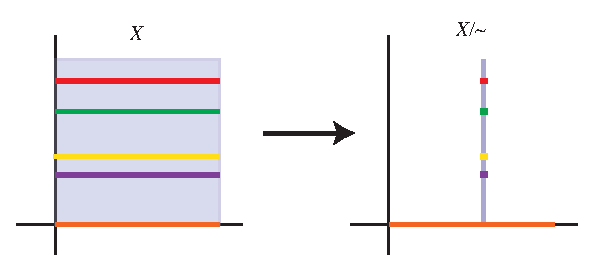
\includegraphics[width=280pt]{images/hausdorffness/IxInonexample}\]
	Points of the same color are identified. Points on the $x$-axis are not separable, so this is a Hausdorff space $X$ and an equivalence relation $\sim$ such that $X/\sim$ is not Hausdorff. 
\end{example}
\begin{example}
	Let $X=\R,$ and set $x \sim y$ if and only if $x=y$ or $x,y>0.$ 
	
	\[
	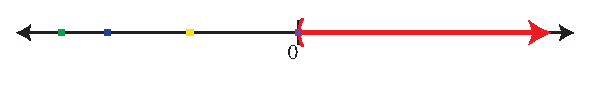
\includegraphics[width=360pt]{images/hausdorffness/r_nonexample}\]
	
	Let $p>0.$ Then $[p],[0]\in X/\sim$. Let $U \subseteq X/\sim$ be an open set containing $[0].$ We claim that $[p]\in U$. To see why, note that $\pi^{-1}(U)$ is an open subset of $\R$ containing $0$. Hence, there exists $q \in \pi^{-1}(U)$ such that $q>0.$ Therefore, $q \sim p \Rightarrow [q]=[p]\in U$, and $X/\sim$ is not Hausdorff. 
\end{example}

Note: this proves that the continuous images of a Hausdorff space need not be Hausdorff! 
 


%!TEX root = ../Notes.tex
\section{Normalness} 
\begin{definition}
	Let $(X,F_x)$ be a topological space. We say $X$ is \textbf{normal} if for every pair of disjoint closed sets $A,B \subseteq X$, there exist disjoint open sets $U,V\subseteq X$ such that $A \subseteq U$ and $B \subseteq V$. 
\end{definition}

On Homework 2, we proved that metric spaces are normal. 
\begin{example}
	Consider $\R$ with a topology $F$ defined by a basis of all sets of the form $(a,b)$ plus all sets of the form $(a,b)\cap \Q.$ This is known as the \textbf{rational topology}, and it is finer than the usual topology. As an exercise, you can prove that that this collection of sets really form the basis of a topology. (Use the basis lemma.) 
	
	We want to show that $(\R,F)$ is Hausdorff. This is easy, because $F$ contains the usual topology on on $\R$, which is Hausdorff. 
	
	Next, we will show that $(\R,F)$ is not normal. To see why, let $A=\R\setminus\Q.$ Then $A$ is closed, because $\Q$ is contained in $F$. Let $B=\{47\}.$ Suppose there exist $U,V \in F$ such that $A \subseteq U,$ and $B \subseteq V$. Then there exists $\epsilon>0$ such that $(47-\epsilon,47+\epsilon)\cap Q \subseteq V$. 
	
	Let $p \in (47-\epsilon,47+\epsilon)$ such that $p \not\in \Q.$ Then $p \in U$ because $p \not\in \Q$. So, there exists $\delta>0$ such that $(p-\delta,p+\delta) \subseteq U$. 
	
	Now, there must exist a point in $x \in (p-\delta,p+\delta)\cap((47-\epsilon,47+\epsilon) \cap \Q).$ But then $x \in U \cap V$, and so $U \cap V \neq \emptyset$. This proves that $(\R,F)$ is not a normal space. 
\end{example}

In particular, we have shown that a space can be Hausdorff but not normal. Under what conditions \emph{must} a Hausdorff space be normal?
\begin{lemma}
	If $(X,F_x)$ is Hausdorff and compact, then $X$ is normal. 
\end{lemma}
\setcounter{subfigure}{0} 
\begin{proof}
	{Comic-book style} 
	\begin{figure}
		[h!] 
		\begin{center}
			\subfigure[Let $A$ and $B$ be closed and disjoint sets.
			\newline Let $a\in A$.] {
			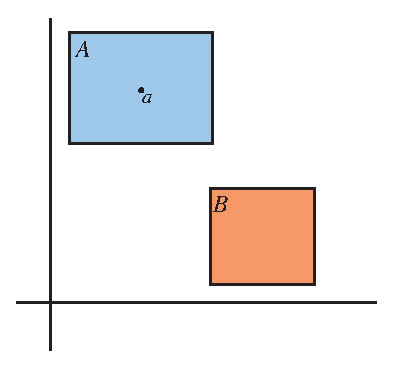
\includegraphics[width=210pt]{images/hausdorffness/hausdorff_comic_1}} \subfigure[Each point in $B$ can be separated from $a$ by an open set. This forms an open cover. Take a finite subcover.] {
			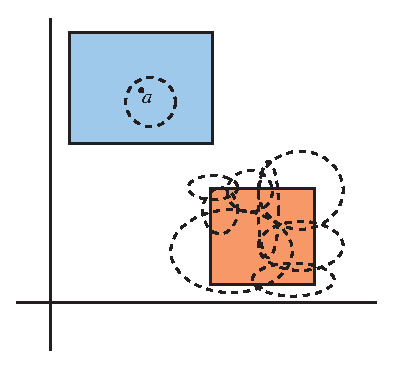
\includegraphics[width=210pt]{images/hausdorffness/hausdorff_comic_2}} 
		\end{center}
	\end{figure}
	\begin{figure}
		\begin{center}
			\subfigure[Repeat for each $a\in A$. This makes an open cover of $A$ and a lot of finite open covers of $B$.] {
			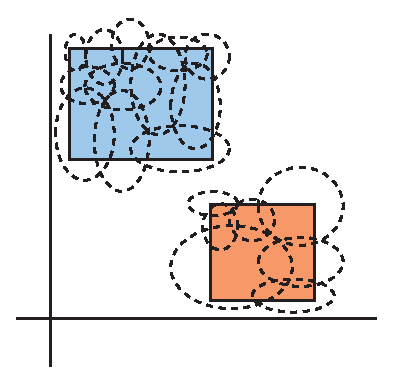
\includegraphics[width=210pt]{images/hausdorffness/hausdorff_comic_3}} \subfigure[Take the intersection of all of the covers of $B$. It's disjoint from the cover of $A$, so $A$ and $B$ are separated by open sets, so $X$ is normal.] {
			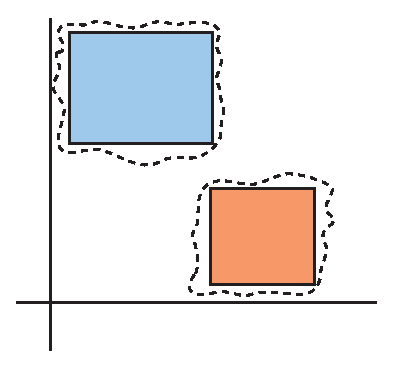
\includegraphics[width=210pt]{images/hausdorffness/hausdorff_comic_4}} 
		\end{center}
	\end{figure}
	\newpage 
\end{proof}
\vskip1cm

Now for the real proof. 
\begin{proof}
	Let $A$ and $B$ be disjoint closed subsets of $X$. Then $A$ and $B$ are compact because $X$ is compact. Let $a \in A$. For every $b \in B$, there exist open sets $U_b$ and $V_b$ such that $a \in U_b$ and $b \in V_b,$ and $U_b \cap V_b = \emptyset.$ Then $\{V_b \mid b \in B\}$ is an open cover of $B$. Since $B$ is compact, we can choose a finite subcover $\{V_{b_1},\ldots,V_{b_n}\}.$ Let $U_a=\cap_{i=1}^n U_{b_i}$. For every $a \in A$, $U_a \in F_x$ and $a \in U_a.$ Let $V_a=\cup_{i=1}^n V_{b_i}$. Then $B \subseteq V_a \in F_x$. 
	
	We claim that $U_a \cap V_a = \emptyset$ for all $a \in A$. To see why, note that $\left( \cap_{i=1}^n U_{b_i}\right) \cap \left( \cup_{i=1}^n V_{b_i} \right) = \emptyset$ because for all $i$, $U_{b_i} \cap V_{b_i}=\emptyset.$
	
	Now, $\{U_a \mid a \in A\}$ is an open cover of $A$. Since $A$ is compact, this cover has a finite subcover $\{U_{a_1},\ldots,U_{a_m}\}$. Now, $V=\cap_{i=1}^{m}V_{a_i}$ is open and $B \subseteq V$. For all $i=1,\ldots,m,$ $U_{a_i}\cap \left( \cap_{i=1}^m V_{a_i} \right) = \emptyset$ because for all $i=1,\ldots,m$, $U_{a_i} \cap V_{a_i}=\emptyset$. 
	
	Let $U=\cup_{i=1}^m U_{a_i} \in F_x$. Then $A \subseteq U$ and $U \cap V = \emptyset$ because $U_{a_i} \cap V_{a_i}=\emptyset$ for all $i$.
	
	Therefore, $X$ is normal. 
\end{proof}
\begin{theorem}
	Let $(X,F_X)$ be a compact and Hausdorff topological space. If $(Y,F_Y)$ is a topological space and $f : X \to Y$ is continuous, onto, and closed, then $(Y,F_Y)$ is compact and Hausdorff. 
\end{theorem}
\begin{proof}
	From previous notes, since $f$ is continuous and $X$ is compact, $Y$ is compact.
	
	So now consider Hausdorff:
	
	Let $p,q \in Y$ such that $p \neq q$. As $f$ is onto, $\exists \ a,b \in X$ such that $f(a) = p$ and $f(b) = q$. As $X$ is Hausdorff, $\{a\}$ and $\{b\}$ are closed. As $f$ is closed, $f(\{a\}) = \{p\}$ and $f(\{b\}) = \{q\}$ are closed. Therefore, as $f$ is continuous, $f^{-1}(\{p\})$ and $f^{-1}(\{q\})$ are closed, and are clearly disjoint.
	
	As $X$ is both compact and Hausdorff, it is also normal. So $\exists \ U,V \in F_X$ such that $f^{-1}(\{p\}) \subseteq U$, $f^{-1}(\{q\}) \subseteq V$, and $U \cap V = \emptyset$. As these sets are open, $A = U^c$ and $B = V^c$ are closed. As $f$ is closed, $f(A)$ and $f(B)$ are also closed, and hence $f(A)^c$ and $f(B)^c$ are open.
	
	Suppose that $p \in f(A)$. Then for some $x \in A$, $f(x) = p$. But then $x \in f^{-1}(\{p\}) \subseteq U = A^c$. So $x \in A \cap A^c$, which is a contradiction. So $p \in f(A)^c$, and by a similar argument, $q \in f(B)^c$.
	
	Now suppose that $c \in f(A)^c \cap f(B)^c$. So, as $f$ is onto, there exists some $d \in X$ such that $f(d) = c$. As $c \notin f(A)$, $d \notin A$, so $d \in U$. Similarly, as $c \notin f(B)$, $d \in V$. But then $d \in U \cap V = \emptyset$. This is a contradiction, so no such $c$ exists, and $f(A)^c \cap f(B)^c = \emptyset$.
	
	So $f(A)^c$ and $f(B)^c$ are disjoint open sets with $p \in f(A)^c$ and $q \in f(B)^c$. As such open sets exist for all $p,q \in Y$, $Y$ is Hausdorff.
	
	Therefore $Y$ is compact and Hausdorff, as desired. 
\end{proof}
 


%!TEX root = ../Notes.tex
\section{Connectedness} 
\subsection{Connected Sets and Spaces} 
\begin{definition}
	$(X,F_X)$ is a topological space. Then $X$ is \textbf{disconnected} if $X$ has a proper, nonempty, clopen subset. Otherwise, $X$ is \textbf{connected}.
	
	Equivalently, $X$ is disconnected if there exist nonempty, disjoint $A,B \in F_X$ such that $A \cup B = X$. $A$ and $B$ are called a separation of $X$. 
\end{definition}

Recall from Math 131 that $A \subseteq \R$ is connected iff $A$ is an interval.
\begin{theorem}
	Let $f : (X,F_X) \to (Y,F_Y)$ be continuous. Then $X$ is connected only if $f(X)$ is connected. 
\end{theorem}
\begin{proof}
	Suppose that $U,V \in F_Y$ are separating sets of $f(X)$. Then, as $f$ is continuous, $f^{-1}(U)$ and $f^{-1}(V)$ are open. As $U$ and $V$ cover $f(X)$, $f^{-1}(U)$ and $f^{-1}(V)$ cover $X$. Furthermore, suppose that $x \in f^{-1}(U) \cap f^{-1}(V)$. Then $f(x) \in U \cap V$, and $f(x) \in f(X)$. However, this contradicts the assumption that $U$ and $V$ are separating sets. So $f^{-1}(U)$ and $f^{-1}(V)$ are disjoint open sets that cover $X$, so they are a separating set. But $X$ is connected, so this is a contradiction. Hence, no such $U$ and $V$ exist, and $f(X)$ is also connected. 
\end{proof}

Are the following connected? 
\begin{itemize}
	\item $\R$ with the finite complement topology - Yes. Let $U$ be some proper, nonempty open subset of $\R$. Then it is infinite, so its complement does not have finite complement. Therefore, its complement is not open. So there are no proper, nonempty clopen sets, and the topology is connected. 
	\item $\R$ with the half-open interval topology - No. Let $U = [0,\infty)$ and $V = (-\infty,0)$. These are open as $U = \bigcup_{n\in \N} [0,n)$ and $V = \bigcup_{n \in \N} [-n,0)$, and the arbitrary union of basis elements is open. Furthermore, they are clearly disjoint, and cover $\R$. 
\end{itemize}

We can also define (dis)connectedness for subsets of a topological space. 
\begin{definition}
	$(X,F_X)$ is a topological space. $S \subseteq X$ is \textbf{disconnected} if and only if there exist $U,V \in F_X$ such that $(U \cap S) \cap (V \cap S) = \emptyset$, $U \cap S, V \cap S \neq \emptyset$ and $S \subseteq U \cup V$. Note that this does not require $U \cap V = \emptyset$. 
\end{definition}
\begin{smallfact}
	$(X, F_X)$ is connected if and only if $\forall \ f : X \to Y$ where $Y$ has the discrete topology and $f$ is continuous, then $f$ constant. 
\end{smallfact}
\begin{proof}
	\begin{itemize}
		\item[$(\Rightarrow)$] Suppose $(X,F_x)$ is connected and that $\exists \ f : X \to Y$ where $Y$ has the discrete topology, such that $f$ is continuous and not constant. So there exist $p,q \in Y$ such that $p \neq q$ and $f^{-1}(\{p\}), f^{-1}(\{q\}) \neq \emptyset$. Therefore, $U = f^{-1}(\{p\})$ and $V = f^{-1}(\{p\}^c) \supseteq f^{-1}(\{q\})$ have $U,V \neq \emptyset$. As every set is open in the discrete topology and $f$ is continuous, $U,V \in F_X$. Furthermore, as $\{p\} \cap \{p\}^c = \emptyset$, $U \cap V = \emptyset$, and $U \cup V = f^{-1}(Y) = X$. So $U$ and $V$ separate $X$. However, $X$ is connected, so this is a contradiction, and no such $f$ exists. 
		\item[$(\Leftarrow)$] Suppose that $f : X \to Y$ is constant for all continuous $f$ where $Y$ has the discrete topology and that $X$ is disconnected. Then there exist separating sets $A,B \in F_X$. Define $Y = \{0,1\}$ with the discrete topology and $f : X \to Y$ as
		\[f(x) = \left\{ 
		\begin{array}{cc}
			0 & x \in A \\
			1 & x \in B
		\end{array}
		\right.\]
		Then, as $f^{-1}(\{0\}) = A \in F_X$, $f^{-1}(\{1\}) = B \in F_X$, $f^{-1}(\emptyset) = \emptyset \in F_X$ and $f^{-1}(Y) = X \in F_X$, $f^{-1}(U) \in F_X$ for all $U \subseteq Y$ such that $U$ is open. So $f$ is continuous. Furthermore, as $A,B \neq \emptyset$, there exist $a \in A$ and $b \in B$, so $f(a) = 0$ and $f(b) = 1$. Hence $f$ is not constant. Therefore $f : X \to Y$ is a continuous function from $X$ to a space with the discrete topology that is not constant. This contradicts the initial assumption, so $X$ is connected. 
	\end{itemize}
\end{proof}

We now have an Important Lemma about Flowers. 
\begin{lemma}
	Suppose \{$y_j \mid j \in J$\} is a collection of connected subspaces of $X = \displaystyle{\bigcup_{j \in J} y_j}$, and $\displaystyle{\bigcap_{j \in J} y_j} \neq \emptyset$. Then $X$ is connected. 
\end{lemma}
\begin{proof}
	Suppose that $X$ is \textit{dis}connected. Then $X$ has a separation, $U, V$. \placeholder (draw a flower)
	
	Let $j_0 \in J$. We know that 
	\begin{itemize}
		\item $(U\cap y_{j_0}) \cup (V\cap y_{j_0}) = y_{j_0}$, 
		\item $(U\cap y_{j_0}) \cap (V\cap y_{j_0}) = \emptyset$, 
		\item $(U\cap y_{j_0})$ and $(V\cap y_{j_0})$ are open in $y_{j_0}$, 
		\item $y_{j_0}$ is connected, so either $U \cap y_{j_0} = \emptyset$ or $V \cap y_{j_0} = \emptyset$. 
	\end{itemize}
	Without loss of generality, say $U \cap y_{j_0} = \emptyset$. Then $V \cap y_{j_0} = y_{j_0}$. By the same argument, $\forall j\in J, y_j \subseteq U$ or $y_j \subseteq V$.
	
	But $\displaystyle{\bigcap_{j \in J} y_j} \neq \emptyset$, so there exists $p\in \displaystyle{\bigcap_{j \in J} y_j}$ such that $p\in y_{j_0} \subseteq V$. Thus $\forall j\in J$, $y_j \subseteq V$.
	
	Since $X = \displaystyle{\bigcup_{j \in J} y_j} \subseteq V$, $U, V$ is not a separation of $X$. Thus, $X$ is connected. 
\end{proof}
\begin{theorem}
	Let $(X, F_X)$ and $(Y, F_Y)$ be topological spaces. Then $(X\times Y, F_{X\times Y})$ is connected if and only if both $X$ and $Y$ are connected. 
\end{theorem}
\begin{proof}
	\begin{itemize}
		\item[$(\Rightarrow)$] $\pi_X: X\times Y \longrightarrow X$ and $\pi_Y: X\times Y \longrightarrow Y$ are continuous surjections. Continuous functions preserve connectedness, so $X$ and $Y$ are connected. 
		\item[$(\Leftarrow)$] First, a picture proof. \placeholder The axes are connected, because $X$ and $Y$ are connected. If we make a copy of the axes, shifted over a little bit, that copy is connected too. The union of these shifted axis crosses will be the entirety of $X\times Y$, and their intersection will be nonempty, so $X\times Y$ is connected.
		
		Now for the actual proof. Let $(x_0, y_0) \in X\times Y.$ Since $\{x_0\}\times Y \cong Y$, it is connected (as connectedness is a top. prop.). Similarly, $\{y_0\} \times X$ is connected.
		
		Observe that $(x_0, y_0) \in (\{x_0\}\times Y) \cap (\{y_0\} \times X)$. That is, $(\{x_0\}\times Y) \cap (\{y_0\} \times X) \neq \emptyset$. Then $(x_0, y_0) \in (\{x_0\}\times Y) \cup (\{y_0\} \times X)$ is connected by the Important Flower Lemma. By the same process, we see that $\forall x\in X$, $(X\times \{y_0\}) \cup (\{x\} \times Y)$ is connected.
		
		Note that $(X\times \{y_0\}) \subseteq \displaystyle{\bigcap_{x \in X}(X\times \{y_0\}) \cup (\{x\} \times Y)}$.
		
		\textbf{Claim.} $\displaystyle{\bigcup_{x \in X}(X\times \{y_0\}) \cup (\{x\} \times Y)} = X\times Y$ \textbf{Proof of claim.}
		
		$(\subseteq)$ Clearly $\displaystyle{\bigcup_{x \in X}(X\times \{y_0\}) \cup (\{x\} \times Y)} \subseteq X\times Y$ because $X\times Y$ is the entire space. 
		
		$(\supseteq)$ Let $(x_1, y_1) \in X\times Y$. Then $(x_1, y_1) \in (\{x_1\}\times Y)$. Thus, $\forall x\in X$ and $y\in Y$, $(x,y) \in (\{x\} \times Y) \subseteq {\displaystyle\bigcup_{x \in X}(X\times \{y_0\}) \cup (\{x\} \times Y)}$.
		
		Since $(X\times \{y_0\}) \cup (\{x\} \times Y)$ is connected $\forall x\in X$, and $\displaystyle{\bigcap_{x \in X}(X\times \{y_0\}) \cup (\{x\} \times Y)}\neq \emptyset$, $X\times Y$ is connected by the Important Flower Lemma. 
	\end{itemize}
\end{proof}

\subsection{Connected Components} 
\begin{definition}
	Let $(X, F_X)$ be a topological space and let $p\in X$. Let $\{C_j\mid j\in J\}$ be the set of all connected subspaces of $X$ containing $p$. Then ${\displaystyle\bigcup_{j\in J}C_j}$ is said to be the \textbf{connected component}, $C_p$, of $p$. 
\end{definition}

And now, a series of tiny facts about connected components. 
\begin{smallfact}
	Let $(X, F_X)$ be a topological space. Then, 
	\begin{enumerate}
		\item $\forall p \in X$, $C_p$ is connected. 
		\item If $C_p$ and $C_q$ are connected components, then either $C_p\cap C_q = \emptyset$ or $C_p = C_q$. (That is, connected components partition a space.) 
	\end{enumerate}
	
\begin {proof} 
\begin{enumerate}
	\item $p\in {\displaystyle\bigcap_{j\in J} C_j}$, so $C_p = {\displaystyle\bigcup_{j\in J} C_j}$ is connected by the Important Flower Lemma. 
	\item Suppose $C_p \cap C_q \neq \emptyset$ and let $x\in C_p \cap C_q$. Then $C_p \cup C_q$ is connected by the Important Flower Lemma.
	
	$p\in C_p \cup C_q$, so $C_p \cup C_q \in \{C_j\mid j\in J\}$. Also, $C_p \cup C_q \subseteq C_p$, since $C_p = {\displaystyle\bigcup_{j\in J} C_j}$. So, $C_q \subseteq C_p$. Similarly, $C_p \subseteq C_q$. 
\end{enumerate}
Thus $C_p = C_q$, so we can say $X$ is partitioned by its connected components. 
\end{proof}
\end{smallfact}
\begin{example}
Let $X = \R^2$ with the dictionary topology. Connected components are vertical lines. (Proof is an exercise.) Define $x\backsim y$ ($x, y \in \R^2$) if $x$ and $y$ are in the same connected component. Then $X/\backsim$ = $\R$ with the discrete topology. \\
(Draw your dictionary topology components and $X/\backsim$ here!)\\
\placeholder 
\end{example}

Connectedness is not always intuitive, though. Here's a large example showing that: \textbf{The Flea and the Comb}.

Define the Comb, the Flea, and the space $X$ as follows. 
\begin{itemize}
\item[Comb:] ${\displaystyle\bigcup_{n=0}^{\infty}y_n}$ in $\R^2$ where $y_0 = [0,1]\times\{0\}$ and $\forall n\in \N$, $y_n = \{1/n\} \times [0,1]$. 
\item[Flea:] $\{(0,1)\}$. 
\item[$X$:] Flea $\cup$ Comb with the subspace topology. 
\end{itemize}
\begin{example}
$X$ is connected. 
\end{example}
\begin{proof}
First, we claim that the Comb is connected. Proof: 

$\forall n \in \{0\} \cup \N$, $y_n$ is connected because $y_n \cong [0,1]$. Also, $\forall n \in \N$, $y_0 \cap y_n \neq \emptyset$ (because $(1/n, 0)$ is in both), so $y_0 \cup y_n$ is connected. 

Thus ${\displaystyle\bigcap_{n\in \N}y_0 \cup y_n} \neq \emptyset$, so ${\displaystyle\bigcup_{n=0}^{\infty}y_0 \cup y_n} = {\displaystyle\bigcup_{n=0}^{\infty}y_n} $ and so the Comb is connected by the Important Flower Lemma. 
\begin{flushright}
$\Box$
\end{flushright}

Now we want to show that $X$ is connected. Suppose $U$, $V$ are a separation of $X$. Since the Comb is connected, we can say, WLOG, that Comb $\subseteq U$. Then it must be that Flea $\subseteq V$ because $U$, $V$ are a separation. $V$ is open in $X$, so $\exists \epsilon > 0$ s.t. $B_{\epsilon}((0,1); X) \subseteq V$. Let $n \in \N$ s.t. $n > \frac{1}{\epsilon}$. Then $d((\frac{1}{n}, 1), (0, 1)) = \frac{1}{n} < \epsilon \Rightarrow (1/n, 1) \in B_{\epsilon}((0,1); X) \subseteq V$. Observe that since $Y_n = \{1/n\} \times [0,1]$, $(1/n, 1) \in Y_n$. Thus, $(1/n, 1) \in V \cap Y_n \subseteq V \cap Y \subseteq V \cap U \Rightarrow V \cap U \neq \emptyset$. But this is a contradiction, since we assumed that $U$, $V$ was a separation of $X$. Thus, $X$ is connected. 
\end{proof}

\section{Path-Connectedness} 
\begin{definition}
Let $(X, F_X)$ be a topological space and let $f:[0,1] \rightarrow X$ be continuous. Then we say that $f$ is a \textbf{path} from $f(0)$ to $f(1)$ (Note: it is handy to think of $t \in [0,1]$ as time). 
\end{definition}
\begin{definition}
Let $(X, F_X)$ be a topological space. If $\forall p$, $q \in X$, there exists a path in $X$ from $p$ to $q$ then we say that $X$ is \textbf{path-connected}. 
\end{definition}
\begin{example}
$\R^n$ is path-connected:

Let $a$, $b \in \R^n$ be given. Let $f: I \rightarrow \mathbb{R}^n$ be $f(t) = (1-t)a + bt$. Then $f(0) = a$, and $f(1) = b$. $f$ can be shown to be continuous by performing an involved $\epsilon$-$\delta$ proof. 
\end{example}

Some remarks: 
\begin{enumerate}
\item Connected is a negative definition and path-connected is a positive definition (for connectedness, we are trying to show that a separation \emph{doesn't} exist, so it is easiest to do connectedness proofs by contradiction. For path-connectedness, we are trying to show that a path exists, so path-connectedness proofs are more easily done constructively). 
\item In general, it is easier to prove that a space is disconnected than to prove that it is not path-connected. 
\item In general, it is easier to prove that a space is path-connected than to prove that it is connected. 
\end{enumerate}
\begin{theorem}
If $(X, F_X)$ is path-connected, then $(X, F_X)$ is connected. 
\end{theorem}
\begin{proof}
Suppose there exists a separation $U$, $V$ of $X$. Since $U$, $V$ is a separation of $X$, $U \neq \emptyset$, $V \neq \emptyset$. Let $p \in U$, $q \in V$ be given. Since $X$ is path-connected, $\exists$ a path $f$ from $p$ to $q$. Since paths are continuous by definition, $f$ is continuous, so $f^{-1}(U)$, $f^{-1}(V)$ are open in $[0,1]$. 

\emph{Claim 1:} $f^{-1}(U) \cup f^{-1}(V) = [0,1]$. \\
\emph{Proof of Claim 1:} Let $x \in [0,1]$ be given. Then $f(x) \in X = U \cup V \Rightarrow f(x) \in U$ or $f(x) \in V \Rightarrow x \in f^{-1}(U)$ or $x \in f^{-1}(V) \Rightarrow x \in f^{-1}(U) \cup f^{-1}(V)$. Thus, $[0,1] \subseteq f^{-1}(U) \cup f^{-1}(V) \Rightarrow [0,1] = f^{-1}(U) \cup f^{-1}(V)$ (since $f^{-1}(U)$, $f^{-1}(V) \subseteq [0,1]$).

\emph{Claim 2:} $f^{-1}(U) \cap f^{-1}(V) = \emptyset$. \\
\emph{proof of Claim 2:} Suppose $\exists x \in f^{-1}(U) \cap f^{-1}(V)$. Then $x \in f^{-1}(U) \Rightarrow f(x) \in U$, and $x \in f^{-1}(V) \Rightarrow f(x) \in V$, so $f(x) \in U \cap V$, which is impossible since we are assuming that $U$ and $V$ are a separation of $X$. Thus, $f^{-1}(U) \cap f^{-1}(V) = \emptyset$.

Observe that since $f$ is a path from $p$ to $q$, $f(0) = p$ and $f(1) = q$, so $0 \in f^{-1}(U)$, $1 \in f^{-1}(V)$ so $f^{-1}(U)$ and $f^{-1}(V)$ are non-empty and proper. Thus, since $f^{-1}(U) \cap f^{-1}(V) = \emptyset$ and $f^{-1}(U) \cup f^{-1}(V) = [0,1]$, $f^{-1}(U)$ and $f^{-1}(V)$ form a separation of $[0,1]$. But this is a contradiction, since we know from Math 131 that $[0,1]$ is connected. Thus, $(X, F_X)$ must be connected. 
\end{proof}

Recall the example of the flea and the comb. We showed that the flea and comb is connected. 
\begin{theorem}
The flea and comb is not path-connected. 
\end{theorem}
\begin{proof}
We want to show that $\nexists$ a path from the flea to $(0,0)$. 

Suppose $\exists$ a path $f$ from the flea to $(0,0)$. Let $p =$ flea. Then $f^{-1}(\{p\})$ is not empty because $f(0) = p$ by the definition of $f$. Similarly, by the definition of $f$, $f(1) = (0,0) \neq p$, so $f^{-1}(\{p\})$ is proper as well. Observe that since $\{p\}$ is closed in $X$ and $f$ is continuous, $f^{-1}(\{p\})$ is closed.

We'd like to show that $f^{-1}(\{p\})$ is open, since then it would be a nontrivial clopen subset of the flea and the comb. This implies that the set is not connected, a contradiction.

Let $y \in f^{-1}(\{p\})$ be given. 

%\\ \emph{WTS:} $\exists \epsilon > 0$ s.t. $B_{\epsilon}(y; [0,1]) \subseteq f^{-1}(\{p\})$.
Observe that $B_{\frac{1}{2}}(p; X)$ is open in $X$. Since $f$ is a path, $f$ is continuous, so $f^{-1}(B_{\frac{1}{2}}(p; X))$ is open in $[0,1]$. Since $y \in f^{-1}(\{p\})$, $f(y) = p \in B_{\frac{1}{2}}(p; X) \Rightarrow y \in f^{-1}(B_{\frac{1}{2}}(p; X))$. Thus, since $f^{-1}(B_{\frac{1}{2}}(p; X))$ is open in $[0,1]$, $\exists \epsilon > 0$ s.t. $B_{\epsilon}(y; [0,1]) \subseteq f^{-1}(B_{\frac{1}{2}}(p; X))$.

%\\ \emph{WTS:} $B_{\epsilon}(y; [0,1]) \subseteq f^{-1}(\{p\})$.
Let $z \in B_{\epsilon}(y; [0,1])$. If $f(z) = p$, then $B_{\epsilon}(y; [0,1]) \subseteq f^{-1}(p)$ and so $f^{-1}(p)$ is open, completing the proof.

Suppose $f(z) \neq p$. Since $z \in B_{\epsilon}(y; [0,1])$, $z \in f^{-1}(B_{\frac{1}{2}}(p; X))$, so $f(z) \in B_{\frac{1}{2}}(p; X)$ (so $d(f(z), p) < \frac{1}{2}$). Since $Y_0 = [0,1] \times \{0\}$, for each $q \in Y_0$, $d(p,q) \geq 1 \Rightarrow q \not\in B_{\frac{1}{2}}(p; X)$. Thus, $f(z) \not\in Y_0$. Thus since $f(z) \neq p$, $\exists n \in \mathbb{N}$ s.t. $f(z) \in Y_n$.

There exists $r\in \R-\Q$ such that $0 < r < \frac{1}{n}$. Define sets $A, B\subseteq f\left( B_{\epsilon} (y;[0,1]) \right)$, as
\[A = \left\{ (x,y)\in f\left( B_{\epsilon} (y;[0,1]) \right) | x< r\right\} \hspace{.15in} \text{and} \hspace{.15in} B = \left\{ (x,y)\in f\left( B_{\epsilon} (y;[0,1]) \right) | x> r\right\}\]
We next show that $A$ and $B$ are a separation for $f\left( B_{\epsilon} (y;[0,1]) \right)$. To this end, we'll need to show that $A$ and $B$ are disjoint, proper and non-empty, that their union is the entire set, and that they're are both clopen.

We note that $A\cap B = \emptyset$ by definition. We know that $f(z)\in B$, and $p\in A$, so neither set will be empty and both will be proper.

Next, we want to show that $A\cup B = f\left( B_\epsilon (y;[0,1]) \right)$. Certainly $A\cup B \subseteq f\left( B_{\epsilon} (y;[0,1]) \right)$. Now let $(x, f(x)) \in f\left( B_{\epsilon} (y;[0,1]) \right)$. We know that $f(x) \neq 0$, and in fact $x = \frac{1}{m}$ for some $m\in \N$. Then $x\neq r$, so $x\in A\cup B$ and we're done.

Next we want to show that $A$ is open in $f(B_{\epsilon} (y;[0,1]))$. We know that $\{(x,y) | x<r \}$ is open in $\R^2$, the half plane to the left of $r$. It follows using the subspace topology that $A = \{ (x,y) | x< r \} \cap f\left( B_{\epsilon} (y;[0,1]) \right)$ is open in $f\left( B_{\epsilon} (y;[0,1] ) \right)$. Similarly, $B$ is open in $f\left( B_{\epsilon} (y;[0,1] ) \right)$. Since each is the other's compliment in $f\left( B_{\epsilon} (y;[0,1] ) \right)$, then both are also closed.

We've hence shown that $A$ and $B$ are a separation of $f\left( B_{\epsilon} (y;[0,1] ) \right)$. This is a contradiction, since $B_{\epsilon} (y;[0,1])$ is connected and $f$ is continuous, and thus we've disconnected $B_{\epsilon}(y;[0,1])$. We conclude that $f(z) = p$, for all such $z\in B_{\epsilon}(y;[0,1])$. 

Therefore $B_{\epsilon} (y;[0,1]) \subseteq f^{-1}(\{ p\})$, so $f^{-1} (\{p\})$ is open. So $f^{-1}( \{ p \} )$ is a clopen, non-empty, proper subset of $[0,1]$. This is a contradiction, so we conclude that there does not exist a path in $X$ from $p$ to $(0,0)$ (or anywhere). 
\end{proof}

The point of the whole example is to show that path-connected is stronger than connected. We knew already that path-connected implies connected, and now we see that connected doesn't necessarily imply path-connected.

It turns out that it's useful to have a way to combine paths. 
\begin{definition}
Let $f,g$ be paths in a topological space $(X,F_X)$ such that $f(1) = g(0)$. Then we define $f\ast g : I \to X$ by
\[ (f\ast g )(t) = 
\begin{cases}
f(2t) & 0 \leq t\leq \frac{1}{2} \\
g(2t-1) & \frac{1}{2} \leq t \leq 1 
\end{cases}
\]
\end{definition}

Intuitively what's happening is that we're connecting two paths while speeding things up, creating a new single path parametrized from 0 to 1 from two paths which were parametrized from 0 to 1.
\begin{smallfact}
$f\ast g$ is a path from $f(0)$ to $g(1)$. 
\end{smallfact}
\begin{proof}
By the Pasting Lemma\footnote{HW3 \#1, which states that if we have two continuous functions with closed sets as domains, and they agree over the intersection of these domains, then the combined function is continuous}, since $[0,\frac{1}{2}]$ and $[\frac{1}{2},1]$ are closed subsets under $[0,1]$, and $f(2 (\frac{1}{2} )) = f(1) = g(0) = g(2 (\frac{1}{2}) - 1 )$, $f\ast g$ is continuous. So $f\ast g$ is a path. Since $(f\ast g)(0) = f(0)$ and $(f\ast g) (1) = g(1)$, then $f\ast g$ is a path from $f(0)$ to $f(1)$. 
\end{proof}

This definition also allows us to create an analogue to the flower lemma. 
\begin{theorem}
[Flower Lemma for Path-connected] Let $X = \cup_{i\in I} Y_i$ such that $\forall i\in I$, $Y_i$ is path-connected, and $\cap_{i\in I} Y_i \neq \emptyset$. Then $X$ is path-connected. 
\end{theorem}
\begin{proof}
Let $a,b\in X$. If $\exists n\in I$ such that $a,b\in Y_n$, then there exists a path from $a$ to $b$ in $Y_n\subseteq X$. So without loss of generality, suppose that $a\in Y_n, b\in Y_m$, and $m\neq n$. Let $x\in \cap_{i\in I} Y_i$. Then there exists a path $f$ from $a$ to $x$ in $Y_n$, and a path $g$ from $x$ to $b$ in $Y_m$. So $f\ast g$ is a path in $X$ from $a \to b$, and we're done. 
\end{proof}
\begin{corollary}
The product of path-connected spaces is path-connected. 
\end{corollary}
\begin{proof}
The proof is identical to the connected one; the key is the flower lemma. 
\end{proof}
\begin{definition}
Let $(X,F_X)$ be a topological space, and $p\in X$. Let $\{C_j | j\in J\}$ be the set of all path-connected subspaces of $X$ containing $p$. Then $\cup_{j\in J} C_j$ is said to be the \textbf{path-connected component} $C_p$. 
\end{definition}

Some tiny facts about path-connected components:

Let $(X,F_X)$ be a topological space. Then 
\begin{enumerate}
\item $\forall p\in X, C_p$ is path-connected 
\item If $C_p, C_q$ are path-connected components, then either $C_p \cap C_q = \emptyset$, or $C_p = C_q$. In other words, path-connected components partition the set. 
\end{enumerate}
We'll omit this proof, as it is identical to the one presented on connectedness. 
 


%!TEX root = ../Notes.tex
\section{Homotopies} We now have enough background to start talking about geometric (or algebraic) topology.
\begin{definition}
	Let $f$ be a path in $(X,F_X)$, and define $\overline{f} : I \to X$ by $\overline{f} (t) = f(1-t)$. 
\end{definition}

A few remarks: 
\begin{enumerate}
	\item $\overline{f}$ is a path, because it is a composition of continuous functions. 
	\item $\overline{f}$ is a path from $f(1)$ to $f(0)$. 
	\item $f \ast \overline{f} \neq $ the ``identity''. We haven't created an inverse. 
\end{enumerate}
\begin{definition}
	Let $(X,F_X)$ be a topological space, and $a\in X$. We define $e_a: I\to X$ by $e_a (t) = a$ for all $t\in I$. 
\end{definition}

However, note that $f\ast e_a \neq f$. This isn't an identity.
\begin{definition}
	Let $(X,F_X)$ and $(Y,F_Y)$ be top spaces, and let $f_0: X \to Y$ and $f_1:X\to Y$ be continuous. Then we say that $f_0$ is \textbf{homotopic} to $f_1$ if there exists a function $F:X\times I \to Y$, continuous, such that $F(x,0) = f_0 (x)$, and $F(x,1) = f_1(x)$. We say that $F$ is a \textit{homotopy} from $f_0$ to $f_1$, and we write $f_0 \simeq f_1$. 
\end{definition}

This is probably the most important concept in the rest of these notes.

To illustrate homotopies, a couple of pictures.
\begin{figure}[ht!]
    \centering
    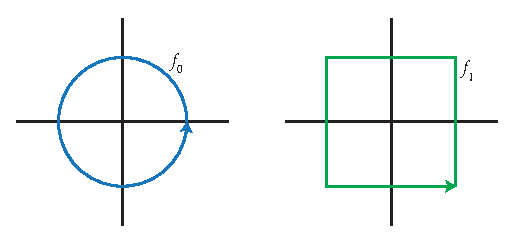
\includegraphics[width=300pt]{images/homotopy/circle_and_square}
\end{figure}

It is visually apparent that one image can be warped to make the other, so $f_0$ and $f_1$ are homotopic. However, homotopic functions need not be homeomorphic. 

These are homotopic, for example:
\begin{figure}[ht!]
    \centering
    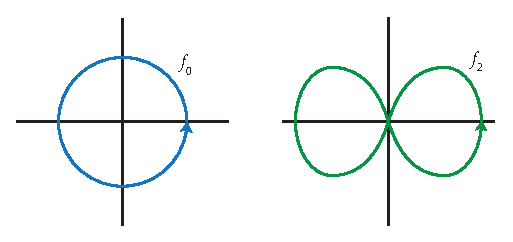
\includegraphics[width=300pt]{images/homotopy/circle_and_infty}
\end{figure}
 
\begin{example}
	Let $X = I$ and $Y = \R^2$. Define $f_0: I \rightarrow \R^2$ by $f_0(x) = (x,0)$, $f_1: I \rightarrow \R^2$ by $f_1(x) = (x,x^2)$, and $F: I \times I \rightarrow \R^2$ by $F(x, t) = t(x, x^2) + (1-t)(x, 0)$.
	
	Observe that $F$ is continuous. Note also that $F(x,0) = (x, 0) = f_0(x)$ and $F(x,1) = (x, x^2) = f_1(x)$.
	
	Thus $F$ is a homotopy. 
\end{example}

\subsection{Drawing Homotopies}

How to draw a homotopy: 
\begin{figure}[ht!]
    \centering
    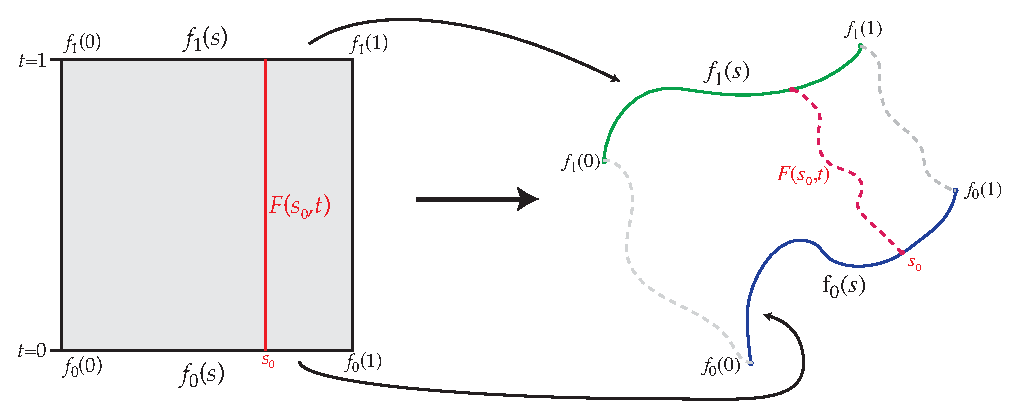
\includegraphics[width=200pt]{images/homotopy/how_to_homotope}
\end{figure}

The image of a vertical segment in the square is the path taken by the $x$ coordinate of that segment during the homotopy.

A few remarks. 
\begin{enumerate}
	\item Suppose $Y$ is not path connected and $f_0(x)$ and $f_1(x)$ are in different path components. Then there does not exist a homotopy from $f_0$ to $f_1$.
	\begin{figure}[ht!]
	    \centering
	    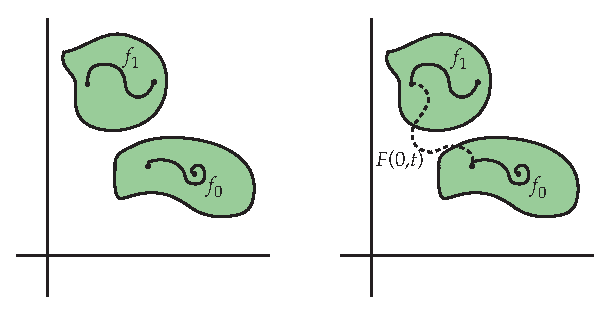
\includegraphics[width=300pt]{images/homotopy/not_path_connected}
	    \caption{If $f_0$ and $f_1$ were homotopic, then $F(0,t)$ would be a path from $f_0(0)$ to $f_1(0)$.  But $f_0$ and $f_1$ are in different path components.}
    \end{figure}
	\item If $Y$ is path connected and $f_0$ and $f_1$ are paths in $Y$, then $f_0 \simeq f_1$. Homotope (the verb!) $f_0$ to its initial point, move it to the initial point of $f_1$ and then stretch it back out into $f_1$.) 
	\begin{figure}[ht!]
	    \centering
	    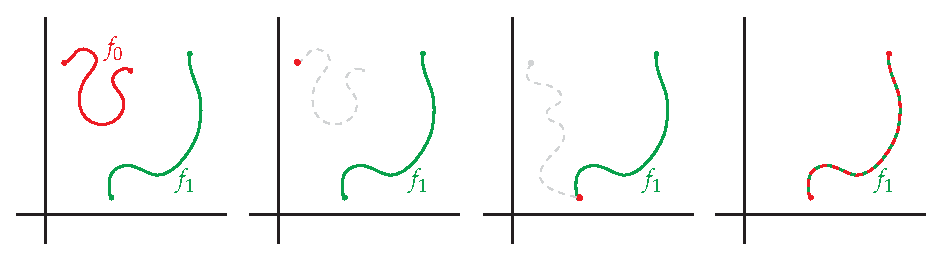
\includegraphics[width=450pt]{images/homotopy/paths_are_homotopic}
    \end{figure}
\end{enumerate}
\begin{example}
	Let $Y = \R^2 - \{(\frac{1}{2}, \frac{1}{3})\}$. Define $f_0: I \rightarrow Y$ by $f_0(s) = (s,s^2)$, and $f_1: I \rightarrow Y$ by $f_1(s) = (s,s).$ Because there's a hole in $Y$, we won't be able to just bend $f_0$ over to $f_1$.
	
	Define $G: I \times I \rightarrow Y$ by $G(s,t) = f_0((1-t)s)$. Observe that $G$ is continuous, and $G(s,0) = f_0(s)$ and $G(s,1) = f_0(0)$.
	
	Now define $H: I \times I \rightarrow Y$ by $H(s,t) = f_1(ts)$. Observe that $H$ is continuous and $H(s,0) = f_1(0)$ and $H(s,1) = f_1(s)$.
	
	Finally, define $F: I \times I \rightarrow Y$ by 
	\begin{displaymath}
		F(s, t) = \left\{ 
		\begin{array}{lr}
			G(s, 2t) & : t \in [0, \frac{1}{2}]\\
			H(s, 2t-1) & : t \in [\frac{1}{2}, 1] 
		\end{array}
		\right. . 
	\end{displaymath}
	\begin{itemize}
		\item[ $F$ is continuous: ] Let $A = I \times [0, \frac{1}{2}]$ and $B = I \times [\frac{1}{2}, 1]$. Both are closed in $I\times I$.\\
		$A \cap B = I \times \{\frac{1}{2}\}$. $G(s, 2(\frac{1}{2})) = G(s, 1) = f_0(0) = (0,0)$ and $H(s, 2(\frac{1}{2})-1) = H(s, 0) = f_1(0) = (0,0)$.
		
		Since $G$ and $H$ are continuous and agree at $A\cap B$, by the Pasting Lemma, $F$ is continuous.
		
		\item[$F$ is a homotopy : ]
		\[F(s, 0) = G(s, 0) = f_0(s) \qquad\text{and}\qquad F(s, 1) = H(s, 1) = f_1(s) \]
	\end{itemize}
	Thus $F$ is indeed an homotopy, and $f_0$ is homotopic to $f_1$! 
\end{example}

What path does $(1, 1)$ take during the aforementioned homotopy?

- Informally put, it moves down along $f_0$ and climbs back up $f_1$ to its old position.

More formally, 
\begin{displaymath}
	F(1, t) = 
	\begin{cases}
		G(1, 2t) & t \in [0, \frac{1}{2}]\\
		H(1, 2t-1) & t \in [\frac{1}{2}, 1] 
	\end{cases}
	= 
	\begin{cases}
		f_0(1-2t) & t \in [0, \frac{1}{2}]\\
		f_1(2t-1) & t \in [\frac{1}{2}, 1] 
	\end{cases}
	=\overline{ f_0} \ast f_1. 
\end{displaymath}

\subsection{Path Homotopies} 
\begin{definition}
	Let $f_0$ and $f_1$ be paths in $(X, F_X)$ from $a$ to $b$. We say $f_0$ is \textit{path-homotopic} if there exists a homotopy $F$ from $f_0$ to $f_1$ s.t. $\forall t \in I$, $F(0,t) = a$ and $F(1, t) = b$. We say $F$ is a \textbf{path homotopy} and write $f_0 \sim f_1$. 
\end{definition}
\begin{figure}[ht!]
    \centering
    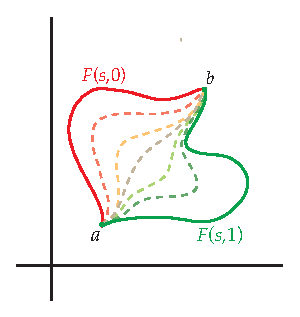
\includegraphics[width=200pt]{images/homotopy/path_homotopy}
\end{figure}
\begin{example}
	Let $X$ be a convex region of $\mathbb{R}^n$, let $a$, $b \in X$, and let $f_0$ and $f_1$ be paths in $X$ from $a$ to $b$. 
\end{example}
Claim: $f_0 \sim f_1$. 
\begin{proof}
	Let $F(s,t) = (1-t)f_0(s) + tf_1(s)$ (Note: we call this the \textbf{straight line homotopy}). Observe that $\forall s \in I$, $F(s,0) = f_0(s)$ and $F(s,1) = f_1(s)$, and that $F$ is continuous, so $F$ is a homotopy from $f_0$ to $f_1$. Now let $t \in I$ be given. Observe that $F(0,t) = (1-t)f_0(0) + tf_1(0) = f_0(0) = a$, and that $F(1, t) = f_0(1) = b$. Thus $\forall t \in I$, $F(0,t) = a$ and $F(1,t) = b$, so $F$ is a path homotopy, and thus $f_0 \sim f_1$. 
\end{proof}
\begin{example}
	Let $X \cong D^2$, let $a, b \in X$, and let $f_0$ and $f_1$ be paths in $X$ from $a$ to $b$. Then $f_0 \sim f_1$. 
\end{example}
\begin{proof}
	Let $g: X \rightarrow D^2$ be a homeomorphism. Let $F: (I \times I) \rightarrow D^2$ be the straight line homotopy in $D^2$ from $g \circ f_0$ to $g \circ f_1$ (Note: $D^2$ is a convex region of $\R^2$, so by the last example we can use the straight line homotopy here).
	
	First, we need to show that $g^{-1} \circ F$ is continuous. Note that $F$ is continuous since $F$ is a homotopy. Note also that since $g$ is a homeomorphism, $g^{-1}$ is continuous. Thus $g^{-1} \circ F$ is the composition of continuous functions, and hence $g^{-1} \circ F$ is continuous.
	
	Now we need to show that $g^{-1} \circ F$ is a homotopy from $f_0$ to $f_1$.
	
	First, observe that $\forall s \in I$, $(g^{-1} \circ F)(s,0) = g^{-1}((1-0)g(f_0(s)) + (0)g(f_1(s))) = g^{-1}(g(f_0(s))) = f_0(s)$ since $g$ is a bijection, and similarly $(g^{-1} \circ F)(s, 1) = f_1(s)$. Thus, since $g^{-1} \circ F$ is continuous, $g^{-1} \circ F$ is a homotopy from $f_0$ to $f_1$.
	
	Lastly, we need to show that $g^{-1} \circ F$ is a \emph{path} homotopy.
	
	Note that $\forall t \in I$, $(g^{-1} \circ F)(0, t) = g^{-1}((1-t)g(f_0(0)) + tg(f_1(0))) = g^{-1}((1-t)g(a) + tg(a)) = g^{-1}(g(a)) = a$ since $g$ is a bijection. Similarly, $\forall t \in I$, $(g^{-1} \circ F)(1,t) = b$. Thus, since $g^{-1} \circ F$ is a homotopy from $f_0$ to $f_1$, $g^{-1} \circ F$ is a path homotopy, and thus $f_0 \sim f_1$. 
\end{proof}
\begin{theorem}
	Let $(X, F_X)$ be a topological space and let $a$, $b \in X$ be given. Then $\sim$ is an equivalence relation of paths in $X$ from $a$ to $b$. 
\end{theorem}
\begin{proof}
	In order to show $\sim$ is an equivalence relation, we need to show that $\sim$ is reflexive, symmetric, and transitive. 
	\begin{itemize}
		\item[Reflexive:] If $f$ is a path in $X$ from $a$ to $b$, let $F: (I \times I) \rightarrow X$ be given by $F(s,t) = f(s)$. Note that $F$ is a homotopy from $f$ to $f$ since, $\forall s \in I$, $F(s,0) = f(s)$ and $F(s,1) = f(s)$ and $F$ is continuous since $f$ is continuous. Observe that $\forall t \in I$, $F(0, t) = f(0) = a$ and $F(1, t) = f(1) = b$, so $F$ is a path homotopy and $f \sim f$. Thus, $\sim$ is reflexive. 
		\item[Symmetric:] Suppose that $f_1 \sim f_2$. Then there exists a path homotopy $F$ from $f_1$ to $f_2$ . Define $F': (I \times I) \rightarrow X$ given by $F'(s,t) = F(s, 1-t)$, $\forall (s,t) \in (I \times I)$. Note that $F'$ is continuous since $F$ is continuous so $F'$ is a composition of continuous functions. Recall that $F$ is a homotopy from $f_1$ to $f_2$, and thus $F'$ is a homotopy from $f_2$ to $f_1$ since, $\forall s \in I$, $F'(s, 0) = F(s, 1) = f_2(s)$ and $F'(s, 1) = F(s, 0) = f_1(s)$. Now observe that $\forall t \in I$, $F'(0,t) = F(0,1-t) = a$ and $F'(1,t) = F(1, 1-t) = b$, since $F$ is a path homotopy. Thus, $F'$ is a path homotopy, and thus $f_2 \sim f_1$, so $\sim$ is symmetric. 
		\item [Transitive:] Suppose that $f_1$, $f_2$, and $f_3$ are paths in $X$ from $a$ to $b$ s.t. $f_1 \sim f_2$ and $f_2 \sim f_3$. Since $f_1 \sim f_2$, there exists a path homotopy $F_1$ from $f_1$ to $f_2$, and since $f_2 \sim f_3$, there exists a path homotopy $F_2$ from $f_2$ to $f_3$. Define $F_3: (I \times I) \rightarrow X$ by 
		\begin{displaymath}
			F_3(s,t) = 
			\begin{cases}
				F_1(s,2t) & t \in [0, \frac{1}{2}]\\
				F_2(s,2t - 1) & t \in [\frac{1}{2}, 1] 
			\end{cases}
		\end{displaymath}
		
		Now we must show that $F_3$ is a path homotopy from $f_1$ to $f_3$. Observe that $A = I \times [0, \frac{1}{2}]$ and $B= I \times [\frac{1}{2}, 1]$ are closed in $I \times I$, and $F_1$ and $F_2$ are continuous, so if $F_1(s,t) = F_2(s,t)$ $\forall (s,t) \in A \cap B$, then by the pasting lemma $F_3$ is continuous. Since $A \cap B = I \times \{\frac{1}{2}\}$, and, $\forall s \in I$, $F_1(s, 2(\frac{1}{2})) = F_1(s, 1) = f_2(s)$ and $F_2(s, 2(\frac{1}{2}) - 1) = F_2(s, 0) = f_2(s)$, $F_3$ is continuous by the pasting lemma. Now, observe that $\forall s \in I$, $F_3(s, 0) = F_1(s, 2(0)) = F_1(s, 0) = f_1(s)$ and $F_3(s, 1) = F_2(s, 2(1) - 1) = F_2(s, 1) = f_3(s)$, so $F_3$ is a homotopy from $f_1$ to $f_3$. Now, observe that $\forall t \in I$, 
		\begin{align*}
			F_3(0,t) &= 
			\begin{cases}
				F_1(0,2t) & \mathrm{if }$ $ t \in [0, \frac{1}{2}]\\
				F_2(0,2t - 1) & \mathrm{if }$ $ t \in [\frac{1}{2}, 1] 
			\end{cases}
			\\
			&= 
			\begin{cases}
				a & t \in [0, \frac{1}{2}]\\
				a & t \in [\frac{1}{2}, 1] 
			\end{cases}
		\end{align*}
		(since $F_1$ and $F_2$ are path homotopies), and thus $F_3(0,t) = a$, $\forall t \in I$. Similarly, $\forall t \in I$, $F_3(1,t) = b$. Thus, $F_3$ is a path homotopy from $f_1$ to $f_3$, so $f_1 \sim f_3$, and thus $\sim$ is transitive. 
	\end{itemize}
	Thus, $\sim$ is an equivalence relation of paths in $X$ from $a$ to $b$. 
\end{proof}

Note that the same proof (using only the parts related to continuity and homotopy) works for $\simeq$.
\begin{definition}
	Let $(X, F_X)$ be a topological space and let $a$, $b \in X$ be given. For each path $f$ from $a$ to $b$ in $X$, define $[f]$ to be the \textbf{path homotopy class of f}. 
\end{definition}
\begin{definition}
	Let $f$ be a path in $X$ from $a$ to $b$ and $g$ be a path in $X$ from $b$ to $c$. Define an \textsc{invisible symbol} by $[f][g] = [f \ast g]$. 
\end{definition}

Some remarks: 
\begin{enumerate}
	\item $[f]$, $[g]$, and $[f \ast g]$ are not elements of the same quotient `world' unless $a = b = c$. 
	\item We have to prove that invisible multiplication is well-defined, i.e. if $f \sim f'$ and $g \sim g'$, then we want $[f \ast g] = [f' \ast g']$ because $[f] = [f']$ and $[g] = [g']$. 
\end{enumerate}
\begin{lemma}
	[Important] The product of path homotopy classes is well-defined. Formally, let $(X,F_x)$ be a topological space. Let $f,f'$ be paths in $X$ from $a$ to $b$ and let $g,g'$ be paths in $X$ from $b$ to $c$. Then:
	\[f*g \sim f'*g' \Rightarrow [f][g] = [f'][g']\]
\end{lemma}
\begin{proof}
	We know $f*g$ and $f'*g'$ are paths in $X$ from $a$ to $c$ by a previous result. Let $F$ be the path homotopy from $f$ to $f'$, and let $G$ be the path homotopy from $g$ to $g'$.
	
	At this point, it may be wise to draw a homotopy diagram: 
    \begin{figure}[ht!]
        \centering
        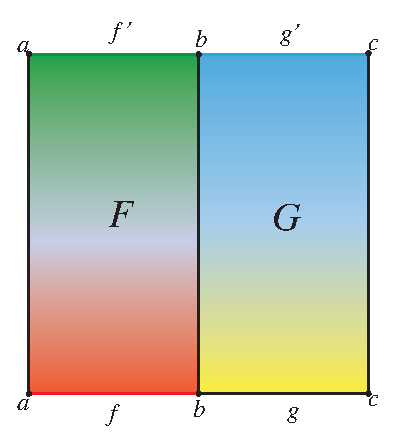
\includegraphics[width=150pt]{images/homotopy/product_well_defined}
    \end{figure}
	
	Define $H:I\times I\to X$ by:
	\[H(s,t) = 
	\begin{cases}
		F(2s,t) & s\in [0,1/2] \\
		G((2s-1),t) & s\in [1/2,1] 
	\end{cases}
	\]
	We claim $H$ is a homotopy from $f*g$ to $f'*g'$. We will now verify the claim. 
	
	We see that:
	\[F(2\cdot(1/2),t) = F(1,t) = b \qquad G(2\cdot(1/2) -1,t) = G(0,t) = b\]
	so by the pasting lemma, it follows that $H$ is continuous.
	
	We now show $H$ gives the desired paths by calculating:
	\[H(0,t) = F(0,t) = a \qquad H(1,t) = G(1,t) = c\]
	so $H(s,[0,1])$ gives a set of paths from $a$ to $c$. 
	
	Finally, we need to prove that $H$ gives a homotopy between the intended paths:
	\[H(s,0) = 
	\begin{cases}
		F(2s,0) & s\in [0,1/2] \\
		G(2s-1,0) & s\in [1/2,1] 
	\end{cases}
	= 
	\begin{cases}
		f(2s) & s\in [0,1/2] \\
		g(2s-1) & s\in [1/2,1] 
	\end{cases}
	= f*g \]
	Similarly:
	\[H(s,1) = 
	\begin{cases}
		F(2s,1) & s\in [0,1/2] \\
		G(2s-1,1) & s\in [1/2,1] 
	\end{cases}
	= 
	\begin{cases}
		f'(2s) & s\in [0,1/2] \\
		g'(2s-1) & s\in [1/2,1] 
	\end{cases}
	= f'*g' \]
	
	Consequently, $H$ satisfies the definition of a path homotopy from $f*g$ to $f'*g'$. We then have that $f*g\sim f'*g'$ so that by definition of the product of paths:
	\[[f][g] = [f*g] = [f'*g'] = [f'][g']\]
	as desired. 
\end{proof}
 


%!TEX root = ../Notes.tex
\section{Loops} We have shown that the product of two path homotopy classes is well defined. For the purposes of defining a group of path homotopy classes, we would like a set of paths whose products have the same endpoints as the original paths. This simplification motivates the two definitions which follow: 
\begin{definition}
	Let $f$ be a path in $X$ such that $f(0) = f(1) = x_0\in X$. Then $f$ is a \textbf{loop} in $X$ based at $x_0$. 
\end{definition}

Note that if $f,g$ are loops in $X$ based at some point $x_0\in X$, then their product $f*g$ is also a loop based at $x_0$. In particular, we then have that $[f],[g]$ and $[f][g] = [f*g]$ are all path-homotopic classes of loops based at $x_0$. 
\begin{definition}
	Let $(X,F_x)$ be a topological space, and let $x_0\in X$. 
	
	Define $\pi_1(X,x_0)$ as the set of path homotopy classes of loops based at $x_0$ endowed with the product of path homotopy classes. We call $\pi_1(X,x_0)$ the \textbf{fundamental group of $X$ based at $x_0$}. 
\end{definition}

\subsection{The Fundamental Group is a Group}

Our ultimate goal is to harness the power of group theory from abstract algebra to study topological spaces. We defined the fundamental group of $X$ based at $x_0$ with the path homotopy class product operation. Naturally, we would like to prove that $\pi_1(X,x_0)$ endowed with the product operation is actually a group. In other words, if $(X,F_x)$ is a topological space with $x_0\in X$, we must prove the following: 
\begin{enumerate}
	\item $\pi_1(X,x_0)$ is closed under the operation $[][]$. In other words, for $[f],[g]\in \pi_1(X,x_0)$, $[f][g] \in \pi_1(X,x_0)$. 
	\item The operation $[][]$ is associative. In other words, given $[f],[g],[h]\in \pi_1(X,x_0)$:
	\[ ([f][g])[h] = [f]([g][h])\]
	\item $\pi_1(X,x_0)$ contains an identity element. In other words, there exists $[e]\in \pi_1(X,x_0)$ such that for all $[f]\in\pi_1(X,x_0)$:
	\[[e][f] = [f][e] = [f]\]
	\item Every element of $\pi_1(X,x_0)$ has an inverse. In other words, given $f\in \pi_1(X,x_0)$, there exists $g\in \pi_1(X,x_0)$ such that:
	\[[f][g] = [g][f] = [e]\]
\end{enumerate}

If $\pi_1(X,x_0)$ satisfies all of these requirements, $\pi_1(X,x_0)$ is a group. 
\begin{lemma}
	[Closure] Let $(X,F_x)$ be a topological space, and let $x_0\in X$. Let $[f],[g]\in \pi_1(X,x_0)$. Then:
	\[[f][g] \in \pi_1(X,x_0)\]
\end{lemma}
\begin{proof}
	We see that:
	\[[f][g] = [f*g]\]
	We know by a previous result that $f*g$ is a path in $X$ from $x_0$ to $x_0$ since $x_0$ is both the starting point of $[f]$ and the endpoint of $[g]$. Consequently, $f*g$ is a loop in $X$ based at $x_0$, so $[f*g] \in \pi_1(X,x_0)$. 
\end{proof}

Next, we will show that path homotopy path products of loops based at a point are associative. 
\begin{lemma}
	[Associativity] Let $(X,F_x)$ be a topological space, and let $x_0\in X$. Let $[f],[g],[h]\in \pi_1(X,x_0)$. Then:
	\[ ([f][g])[h] = [f]([g][h])\]
\end{lemma}
\begin{proof}
	Before actually proving the result, we will explicitly write the formulas for $(f*g)*h$ and $f*(g*h)$:
	\[(f*g)*h = 
	\begin{cases}
		f(4s) & s\in [0,\frac14] \\
		g(4s-1) & s\in[\frac14,\frac12] \\
		h(2s-1) & s\in [\frac12,1] 
	\end{cases}
	\qquad\qquad f*(g*h) = 
	\begin{cases}
		f(2s) & s\in [0,\frac12] \\
		g(4s-2) & s\in[\frac12,\frac34] \\
		h(4s-3) & s\in [\frac34,1] 
	\end{cases}
	\]
	
	We need to construct a homotopy from $(f*g)*h$ to $f*(h*g)$. Before reading the proof, the reader is encouraged to produce a homotopy diagram in the space provided below: \placeholder
	
	Based on our formulas for $(f*g)*h$ and $f*(g*h)$, we parameterize the function $F:I\times I \to X$ by:
	\[F(s,t) = 
	\begin{cases}
		f\left(\frac{4s}{1+t} \right)& s \in \left[ 0,\frac{1+t}4 \right] \\
		g(4s-1-t) & s\in \left[\frac{1+t}4, \frac{2+t}4\right] \\
		h\left(\frac{4s}{2-t} - \frac{2+t}{2-t} \right) & s\in \left[\frac{2+t}4,1\right] 
	\end{cases}
	\]
	
	We claim and will verify that $F$ is a homotopy from $(f*g)*h$ to $f*(g*h)$. We first prove continuity using the pasting lemma as usual. The proof that each of the piecewise parts of $F$ is defined on a closed set is left as a (relatively trivial but tedious) exercise.
	
	We will, however, show that on the boundaries between these regions, the piecewise parts agree. We see: 
	\begin{eqnarray*}
		f\left(\frac{4}{1+t} \cdot \left(\frac{1+t}4\right)\right) & = & f(1) = x_0 \\
		g\left(4\cdot\left(\frac{1+t}4\right)-1-t\right) & = & g(0) = x_0\\
		g\left(4\cdot\left(\frac{2+t}4\right)-1-t\right) & = & g(1) = x_0\\
		h\left(\frac{4}{2-t} \cdot \left(\frac{2+t}4\right)- \frac{2+t}{2-t}\right) & = & h(0) = x_0\\
	\end{eqnarray*}
	so continuity follows by the pasting lemma. Note that we assume $f,g,h$ are continuous so that things like $h\left(\frac{4s}{2-t} - \frac{2+t}{2-t} \right)$ are because compositions of continuous functions are continuous and over $t\in I$, $\frac{4s}{2-t} - \frac{2+t}{2-t}$ is continuous. The justification is similar for the other piecewise parts in the definition of $F$. 
	
	We now verify that $F$ gives a path from $x_0$ to $x_0$ for every fixed $t\in I$. We see that: 
	\begin{eqnarray*}
		F(0,t) & = & f(0) = x_0\\
		F(1,t) & = & h(1) = x_0\\
	\end{eqnarray*}
	as desired.
	
	Finally, we need to show that $F$ provides a homotopy from $(f*g)*h$ to $f*(g*h)$. We have that:
	\[F(s,0) = 
	\begin{cases}
		f\left(4s \right)& s \in \left[ 0,\frac{1+t}4 \right] \\
		g(4s-1) & s\in \left[\frac{1+t}4, \frac{2+t}4\right] \\
		h\left(2s - 1 \right) & s\in \left[\frac{2+t}4,1\right] 
	\end{cases}
	\qquad = \qquad (f*g)*h \]
	\[F(s,1) = 
	\begin{cases}
		f\left(2s \right)& s \in \left[ 0,\frac{1+t}4 \right] \\
		g(4s-2) & s\in \left[\frac{1+t}4, \frac{2+t}4\right] \\
		h\left(4s - 3 \right) & s\in \left[\frac{2+t}4,1\right] 
	\end{cases}
	\qquad = \qquad f* (g*h)\]
	as desired, so $F$ satisfies the three properties of a homotopy from $(f*g)*h$ to $f*(g*h)$.
	
	We have constructed $F(s,t)$ such that $F$ is a homotopy from $(f*g)*h$ to $f*(g*h)$ which implies that $(f*g)*h \sim f*(g*h) \Rightarrow [(f*g)*h] = [f*(g*h)]$. It immediately follows that
	\[ ([f][g])[h] = [f]([g][h])\]
\end{proof}
\begin{lemma}
	[Identity] Let $f$ be a path in $X$ which begins at $x_0$ and ends at $x_1$. Then $f*e_{x_1}\sim f$ and $e_{x_0}* f \sim f$. \footnote{Recall that $\sim$ denotes ``path homotopy."} 
\end{lemma}
\begin{proof}
	We prove that $f* e_{x_1}\sim f$. The other case is similar.
	
	In order to define a homotopy, at $t$, we will ``do'' $f$ for $s\in [0,t(1)+(1-t)\tfrac{1}{2}]$ or, by simplification, $s\in[0,\tfrac{t+1}{2}]$ and $e_{x_1}(t)$ for $s\in [\tfrac{t+1}{2},1]$.
	
	Define $F:I\times I \to X$ by
	\[F(s,t)= 
	\begin{cases}
		f\left(\tfrac{2s}{t+1}\right) & s\in \left[0,\tfrac{t+1}{2}\right] \\\
		e_{x_1} & s\in \left[\frac{t+1}{2},1\right] 
	\end{cases}
	\]
	
	This is: 
	\begin{itemize}
		\item[Continuous:] By the Pasting lemma, as $f, e_{x_1}$ are continuous on closed domains it suffices to check that they agree for $s=\tfrac{t+1}{2}$. This follows easily, as $f\left(\frac{2\tfrac{t+1}{2}}{t+1}\right)=f(1)=x_1$, and $e_{x_1}\left(\tfrac{t+1}{2}\right)=x_1$. 
		\item[A homotopy:]
		\[F(s,0)= 
		\begin{cases}
			f(2s) & s\in\left[0,\tfrac{1}{2}\right]\\
			e_{x_1}(t) & s\in\left[\tfrac{1}{2},1\right] 
		\end{cases}
		= f*e_{x_1}\]
		and
		\[F(s,1)= 
		\begin{cases}
			f(s) & s\in [0,1]\\
			e_{x_1} & s\in [1,1]=f. 
		\end{cases}
		\]
		\item[ A path: ] $F(0,t)=f(0)=x_0$, and $F(1,t)=e_{x_1}=x_1$, hence $F$ is a path. 
	\end{itemize}
	Thus $f*e_{x_1}\sim f$. 
\end{proof}

We've now shown that $\pi_1(X, x_0)$ is closed, has an identity, and the operation is associative, so just showing that inverses exist proves that it's a group. 
\begin{lemma}
	[Inverses] Let $f$ be a path in $X$ from $x_0$ to $x_1$. Then $f*\overline{f}\sim e_{x_0}$ and $\overline{f}*f\sim e_{x_0}$. 
\end{lemma}

The ``wrong" approach: increase the speed over $f$ and $\overline{f}$ and wait at $x_1$. The ``right" approach: travel successively smaller distances along $f$. 
\begin{proof}
	We show only that $f*\overline{f}\sim e_{x_0}$, and the other case follows similarly.
	
	Define $F:I\times I\to X$ by
	\[ F(s,t)= 
	\begin{cases}
		f(2s) & s\in \left[0,\tfrac{1-t}{2}\right] \\
		f(1-t) & s\in \left[\tfrac{1-t}{2},\tfrac{1+t}{2}\right]\\
		\overline{f}(2s-1) & s\in\left[\tfrac{1+t}{2}, 1\right] 
	\end{cases}
	\]
	This is: 
	\begin{itemize}
		\item[Continuous:] Using the pasting lemma, it suffices to check that these functions agree on their (shared) endpoints. As $f(2(\tfrac{1-t}{2}))=f(1-t)$, and $f(2(\tfrac{1+t}{2})-1)=\overline{f}(t)=f(1-t)$, we conclude that $F$ is continuous.
		
		\item[A homotopy:] Let $t=0$,
		\[F(s,0)= 
		\begin{cases}
			f(2s) & s\in [0,1/2]\\
			f(1) & s\in [1/2,1/2] \\
			\overline{f}(2s-1) & s\in [1/2,1] 
		\end{cases}
		=f*\overline{f}(s)\]
		
		For $t=1$,
		\[F(s,1)= 
		\begin{cases}
			f(2s) & s\in [0,0]\\
			f(0) & s\in [0,1]\\
			\overline{f}(2s-1) & s\in [1,1] 
		\end{cases}
		=e_{x_0}.\]
		
		\item[A path:] For $s=0$, $F(0,t)=f(0)=x_0$. And for $s=1$, $F(1,t)=\overline{f}(1)=x_0$. 
	\end{itemize}
	
	For each loop $f$ based at $x_0$, $\overline{f}$ is a loop based at $x_0$. Thus we have shown closure under inverses. 
\end{proof}

It follows that the action $*$ defines a group on the set of loops based at $x_0$.

Observe that the set of paths does not have a group structure, as there is no definition of multiplication between arbitrary paths. 
\begin{example}
	Let $X=\R^n$ and $x_0$ be a point in $X$. Then $\pi_1(X,x_0)=\langle [e_{x_0}]\rangle$. 
\end{example}

The following theorem relates the fundamental group at a point within a path component to the fundamental group of that point in the ambient space: 
\begin{theorem}
	Let $A$ be a path component of a topological space $X$, and let $x_0\in A$. Then:
	\[\pi_1(A,x_0)\cong \pi_1(X,x_0)\]
	(Note that $\cong$ denotes a group isomorphism and not a homeomorphism) 
\end{theorem}

Before proving the theorem, we will cover two quick non-examples of cases where the theorem could break down.

Recall the circle $S^1$ which we can consider as a subspace of $\R^2$. Since $\R^2$ is a simply connected space, the fundamental group at every point is trivial. On the other hand, picking some point $x_0\in S^1$, the loop around the circle cannot be deformed in $S^1$ to the point $x_0$, so $\pi_1(S^1,x_0)$ is non-trivial and hence not isomorphic to $\pi_1(\R^2,x_0)$ if we embed $S^1$ in $\R^2$. The following picture illustrates $S^1$ with the point $x_0$: 
\begin{center}
	\begin{picture}
		(50,50) \put(0,20){\circle*{3}} \put(0,25){$x_0$} \put(0,0){\circle{100}} 
	\end{picture}
	\vspace{10mm} 
\end{center}

This may seem like a counterexample to the theorem, but in $\R^2$, $S^1$ is not a distinct path component of $\R^2$, so the theorem does not apply. Intuitively, by embedding $S^1$ in $\R^2$, the interior of the circle is part of $\R^2$, so we can deform a loop around $S^1$ based at $x_0$ to the trivial loop by ``pulling'' the loop through the middle of the circle, which we could not do when $S^1$ was considered as a space in its own right.

Consider the following diagram: 
\begin{center}
	\begin{picture}
		(50,50) \put(0,20){\circle*{3}} \put(0,25){$x_0$} \put(0,0){\circle{100}} \put(45,0){\circle*{10}} \put(50,5){A} \put(-45,0){\circle*{10}} \put(-53,5){B} 
	\end{picture}
	\vspace{10mm} 
\end{center}
where we have the space $\R^2$ with $A,B$ removed, so loops based at $x_0$ that run around $A,B$ cannot be deformed into the trivial loop. However, when we consider this space embedded in $\R^2$ as a subspace, it is not an entire path component in $\R^2$, so our theorem does not apply. 

We now prove the theorem: 
\begin{proof}
	Define $\varphi:\pi_1(A,x_0)\to \pi_1(X,x_0)$ by:
	\[\varphi([f]_A) = [f]_X\]
	We claim that $\varphi$ is a \emph{group isomorphism}, i.e. that $\varphi$ is a bijection and a group homomorphism. In other words, we need to show that $\varphi$ is injective, surjective and that if $a,b\in\pi_1(A,x_0)$, then $\varphi(ab) = \varphi(a)\varphi(b)$. For those who have not had algebra, the existence of an isomorphism between two groups means that while the two groups may not have the same elements, they have the same algebraic structure. 
	
	Before we actually prove that $\varphi$ satisfies the properties of an isomoprhism, we have to show $\varphi$ is well defined because $\varphi$ is defined in terms of equivalence classes. First, let $f,g$ be loops in $A$ based at $x_0\in A$ such that $f\sim_A g$. Thus there exists a path homotopy in $A$, $F:I\times I\to A,$ from $f$ to $g$. Recall the inclusion map $i:A\to X$ where $i$ is the identity map on $X$ restricted to $A$ and is trivially continuous. Thus we can extend $F$ to the continuous map $i\circ F:I\times I \to X$, and it is easy to see that $i\circ F$ is a path homotopy in $X$ from $f$ to $g$, so $f\sim_X g$. Thus if $[f]_A = [g]_A$, $\varphi([f]_A) = \varphi([g]_A)$, and $\varphi$ is well defined.
	
	We now prove $\varphi$ is injective. Suppose $[f]_A,[g]_A\in \pi_1(A,x_0)$ such that $\varphi([f]_A) = \varphi([g]_A) \Rightarrow [f]_X = [g]_X$. Then there exists $F:I\times I \to X$, a path homotopy from $f$ to $g$ in $X$. Suppose toward a contradiction there exists $(s_0,t_0)\in I\times I$ such that $F(s_0,t_0)\notin A$. Now take a restriction of $F$, $\alpha:[0,s_0] \to X$ defined by $\alpha(s) = F(s,t_0)$. Since $[0,s_0]\cong I$, we can easily reparameterize $\alpha$ over the unit interval as $\beta:I\to X$, giving a path from $x_0$ to $F(s_0,t_0)$, since $F(0,t_0)=x_0$. Consequently, $\alpha(s_0) = \beta(1)\in A$ because $A$ is a path component, so we have a contradiction. Thus every point in $F(I\times I)$ is contained in $A$, so we can define $G:I\times I\to A$ by $G(s,t)=F(s,t)$, so $G$ is a homotopy from $f$ to $g$ in $A$. Consequently, $f\sim_A g \Rightarrow [f]_A = [g]_A$. Thus $\varphi$ is injective.
	
	Next we prove $\varphi$ is surjective. Let $[f]_X\in \pi_1(X,x_0)$, so $f$ is a loop in $X$ based at $x_0$. In other words, $f:I\to X$ is a path containing $x_0$. Since $A$ is a path component, $f(I)\subseteq A$ since we can easily use $f$ to find a path between any two points in $f(I)$. Consequently, $f$ is a loop in $A$ based at $x_0$, so we may state $\varphi([f]_A) = [f]_X$ and $\varphi$ is surjective.
	
	Finally, we prove that $\varphi$ is a homomorphism. Let $[f]_A,[g]_A\in \pi_1(A,x_0)$. We see that:
	\[\varphi([f]_A[g]_A) = \varphi([f*g]_A) = [f*g]_X = [f]_X [g]_X = \varphi([f]_A)\varphi([g]_A)\]
	and $\varphi$ satisfies the definition of a homomorphism.
	
	We have proved that $\varphi$ is a bijective, homomorphism, and is therefore an isomorphism between $\pi_1(A,x_0)$ and $\pi_1(X,x_0)$, so we conclude the two groups are isomorphic, as desired. 
\end{proof}

We now wish to prove a similar result: 
\begin{theorem}
	Let $X$ be a topological space and let $x,y\in X$. Suppose $f:I\to X$ is a path from $x$ to $y$, then $\pi_1(X,x)\cong \pi_1(X,y)$. 
\end{theorem}

Before providing the proof, we will define a key map which we will use again later in the course: 
\begin{definition}
	Define $u_f:\pi_1(X,x)\to \pi_1(X,y)$ by $u_f([g]) = [\overline{f}*g*f]$.\footnote{Technically, $\overline{f}*g*f$ should have some indication of ordering of operations, but we dispense with these designations because we previously proved that $*$ is associative.} 
\end{definition}
We now prove the theorem by showing that $u_f$ is an isomorphism from $\pi_1(X,x)$ to $\pi_1(X,y)$: 
\begin{proof}
	Again, we need to show that $u_f$ is a bijective homomorphism. As usual for functions defined in terms of equivalence classes, we need to show that $u_f$ is actually well defined. 
	
	Suppose that $g,h$ are loops in $X$ based at $x$ such that $g\sim h$, so there exists $F:I\times I\to X$, a path homotopy from $g$ to $h$ in $X$. We want to show that:
	\[\overline{f}*g*f \sim \overline{f}*h*f\]
	Since we know trivally $f\sim f$, $g\sim h$ and $\overline{f}\sim\overline{f}$, using our inverse and identity lemmas for multiplication of path homotopy classes, it is easy to see that $\overline{f}*g*f \sim \overline{f}*h*f$, so $u_f$ is well defined.
	
	Next, we show that $u_f$ is injective. Suppose $g,h$ are loops in $X$ based at $x$ such that $u_f([g]_X) = u_f([h]_X)$. Therefore:
	\[[\overline{f}*g*f] = [\overline{f}*h*f] \Rightarrow \overline{f}*g*f\sim \overline{f}*h*f\]
	so by our important lemma for path homotopies and our inverse/identity lemmas, we have that $g\sim h$ and $u_f$ is injective.
	
	Now we wish to show that $u_f$ is surjective. Let $[g]\in \pi_1(X,y)$. Then $[f*g*\overline{f}]\in \pi_1(X,x)$, and $u_f([f*g*\overline{f}])=u_f([\overline{f}*(f*g*\overline{f})*f])$, which by associativity, inverses, and identity, is precisely $[g]$. Therefore $u_f$ is onto.
	
	Finally, $u_f$ is a homomorphism: let $g,h\in \pi_1(X,x)$. Then 
	\begin{align*}
		u_f([g])u_f([h]) & = [\overline{f}*g*f][\overline{f}*h*f] \\
		& = [\overline{f}*g*h*f] \\
		&= u_f([g*h]) 
	\end{align*}
	
	Therefore, $u_f$ is a group isomorphism. 
\end{proof}

Keep in mind that our overall goal is to show that the fundamental group is a topological invariant. In general, a \emph{topological invariant} is a ``thing'' that takes a value on topological spaces such that every homeomorphic space takes the same value. These invariants are used to distinguish topological spaces.

\subsection{Induced Maps} 
\begin{definition}
	Let $\phi:X\to Y$ be continuous, and $\phi(x_0)=y_0$. Define $\phi_*: \pi_1(X,x_0)\to \pi_1(X,y_0)$ by $\phi_*([f]_X)=[\phi(f)]_Y.$
	
	We say that $\phi_*$ is \underline{induced} by $\phi$. 
\end{definition}
\begin{smallfact}
	[about induced maps] Let $\phi:X\to Y$ and $\phi(x_0)=y_0$. Then $\phi_*$ is well defined. 
\end{smallfact}
\begin{proof}
	Let $f$ and $g$ be loops in $X$ based at $x_0$ such that $f\sim g$. Then there exists $F:I\times I\to X$, a path homotopy from $f$ to $g$. \vspace{.4in}
	
	Consider $\phi(F): I\times I \to Y$. We see that $\phi$ is a composition of continuous functions, so is itself continuous. 
	
	Also, observe that 
	\begin{align*}
		\phi(F(s,0)) =\phi\circ f(s)\\
		\phi(F(s,1)) =\phi\circ g(s)\\
		\phi(F(0,t)) =\phi(x_0) = y_0\\
		\phi\circ F(1,t) =\phi(x_0)=y_0 
	\end{align*}
	
	Thus $\phi(F)$ is a homotopy between $\phi\circ g$ and $\phi\circ f$. So $\phi\circ g\sim \phi\circ f$-- and $\phi_*$ is well defined. 
\end{proof}
\begin{lemma}
	Let $\phi:X\to Y$ be continuous and $\phi(x_0)=y_0$. Then $\phi_*$ is a homomorphism. 
\end{lemma}
\begin{proof}
	Let $[f],[g]\in \pi_1(X,x_0).$ We want to show that $\phi_*([f]_X[g]_X)=\phi_*([f]_X)\phi_*([g]_X$.
	
	Observe that 
	\begin{align*}
		\phi_x([f]_X[g]_X) &= \phi_*([f*g]_X)=[\phi(f*g)]Y \\
		\phi\circ (f*g)(x) &=\phi_* 
		\begin{cases}
			f(2s), &s\in [0,1/2]\\
			g(2s-1) & s\in [1/2,1] 
		\end{cases}
		\\
		&= 
		\begin{cases}
			\phi\circ f(2s) & s\in [0,1/2]\\
			phi\circ g(2s-1) & s\in [1/2,1] 
		\end{cases}
		\\
		&=(\phi\circ f)*(\phi\circ g)(s). 
	\end{align*}
	
	So $\phi\circ f * g=\phi\circ f * \phi\circ g$ and, in particular, 
	\begin{align*}
		\phi(f*g)]_Y &= [(\phi\circ f)*(\phi\circ g)]_Y\\
		& =[\phi\circ f]_Y[\phi\circ g]_Y\\
		& =\phi_*([f]_X)\phi_*([g]_X) 
	\end{align*}
	This concludes the proof of the lemma. 
\end{proof}
\begin{theorem}
	Let $\phi:X\to Y$ be a homeomorphism and $\phi(x_0)=y_0$. Then $\phi_*$ is an isomorphism. 
\end{theorem}

With the previous lemma we showed that $\phi_*$ is a homomorphism. It remains to show that $\phi_*$ is a bijection. 
\begin{proof}
	\begin{itemize}
		\item[1-1:] Let $[f]_X, [g]_X\in \pi_1(X,x_0)$ such that $\phi_* ([f]_X)=\phi_*([g]_X)$. Then by definition of $\phi_*$, $[\phi\circ f]_Y=[\phi\circ g]_Y$. 
		
		Observe that $\phi\circ f\sim_Y \phi\circ g$, so there exists a path homotopy $F$ from $\phi\circ f$ to $\phi\circ g$. Also note that, as $\phi$ is a homeomorphism, $\phi^{-1}:Y\to X$ is continuous.
		
		Hence $\phi^{-1}\circ F:I\times I \to Y$ is a path homotopy from $\phi^{-1}\circ \phi\circ f$ to $\phi^{-1}\phi\circ g.$ Since $g$ is bijective, this is a path homotopy from $f$ to $g$.
		
		\item[Onto:] Recall that $\phi_*:\pi_1(X,x_0)\to \pi_1(Y,y_0)$. Let $[f]\in \pi_1(Y,y_0)$. Then $[\phi^{-1}(f)]_X\in \pi_1(X,x_0)$, because $\phi^{-1}$ is continuous.
		
		$\phi_*([\phi^{-1}(f)]_X)=[\phi\circ \phi^{-1}(f)]_Y$, and as $\phi$ is a bijection, this is $[f]_Y$. 
	\end{itemize}
	
	This illustrates that $\phi_*$ is bijective, and hence is an isomorphism between $X$ and $Y$. 
\end{proof}
\begin{smallfact}
	[about induced homomorphisms] 
	\begin{enumerate}
		\item If $\phi: X\to Y$ and $\psi: Y\to Z$ are continuous, then $(\psi \circ \phi)_* = \psi_* \circ \phi_*$ 
		\item If $i:X\to X$ is the identity, then $i_*$ is the identity isomorphism 
		\item Let $\phi:X\to Y$ be continuous and $f$ a path in $X$ from $p$ to $q$. Then $\phi_\ast \circ u_f = u_{\phi(f)}\circ \phi_*$. (recall, $u_f:\pi_1 (X,p) \to \pi_1(X,q)$ by $u_f([g]) = [\overline{f} \ast g \ast f ] )$ 
	\end{enumerate}
\end{smallfact}
\begin{proof}
	\begin{enumerate}
		\item Note that $(\psi \circ \phi)_\ast : \pi_1(X,x_0 ) \to \pi_1(Z,(\psi \circ \phi)(x_0) )$, a mapping from equivalence classes of loops in $X$ based at $x_0$ to the equivalence classes of loops in $Z$ based at $(\psi\circ \phi)(x_0)$. Let $[f]_X \in \pi_1(X,x_0)$. We then have that $(\psi \circ \phi)_\ast ([f]_X) = [(\psi \circ \phi)(f)]_Z$. Similarly, we note that $(\psi_\ast \circ \phi_\ast ) ([f]_X) = \psi_\ast ([\phi\circ f]_Y) = [\psi \circ \phi \circ f ]_Z = [(\psi \circ \phi)(f) ]_Z$. 
		\item Note that $i_\ast : \pi_1 (X,x_0) \to \pi_1 (X,x_0)$. Let $[f]_X \in \pi_1(X,x_0)$. Then $i_\ast ([f]_X) = [i(f)]_X = [f]_X$. 
		\item We want to show that the following diagram commutes:
		
		$$ 
		\begin{CD}
			\pi_1(X,p) @>u_f>> \pi_1(X,q)\\
			@VV{\phi_\ast} V @VV{\phi_{\ast}}V\\
			\pi_1(Y,\phi(p)) @>u_{\phi(f)}>> \pi_1 (Y,\phi(q)) 
		\end{CD}
		$$
		
		Let $[g]_X\in \pi_1(X,p)$. Then note that 
		\begin{eqnarray*}
			(\phi_\ast \circ u_f)([g]_X) &=& \phi_\ast ([\overline{f}\ast g \ast f]_X) \\
			&= &[ \phi \circ(\overline{f} \ast g \ast f) ]_Y\\
			&=& [(\phi\circ \overline{f}) \ast (\phi \circ g) \ast (\phi\circ f) ] _Y 
		\end{eqnarray*}
		It is easy to show that $\phi \circ \overline{f} = \overline{\phi \circ f}$. To see this, note that $(\phi \circ \overline{f})(s) = \phi \circ \overline{f}(s) = \phi (f(1-s)) = (\phi \circ f) (1-s) = \overline{\phi \circ f}(s)$. So continuing the above expression, we have that: 
		\begin{eqnarray*}
			[(\phi\circ \overline{f}) \ast (\phi \circ g) \ast (\phi\circ f) ] _Y&=& [ (\overline{\phi \circ f}) \ast (\phi \circ g) \ast (\phi \circ f) ] _Y \\
			&=& u_{\phi\circ f} ([\phi \circ g]_Y)\\
			& =& (u_{\phi(f)} \circ \phi_\ast )([g]_X) 
		\end{eqnarray*}
		We then conclude that $\phi_\ast \circ u_f = u_{\phi(f)} \circ \phi_\ast$. 
	\end{enumerate}
\end{proof}
\begin{lemma}
	Suppose $X$ is path-connected, and $x_0 \in X$. Then $\pi_1(X,x_0) $ is trivial if and only if $\forall p,q\in X$ and paths $f,g$ in $X$ from $p$ to $q$, then $f\sim g$. 
\end{lemma}
\begin{proof}
	\text{}\\
	$(\Rightarrow)$ Suppose that $\pi_1 (X,x_0) = \langle [e_{x_0} ] \rangle$. Let $p,q \in X$, and $f,g$ paths in $X$ from $p$ to $q$. Then $f\ast \overline{g}$ is a loop based at $p$. So it is trivial to see that $\pi_1 (X, p) \cong \pi_1 (X,x_0)$ by an earlier theorem, from which we can see that $f\ast \overline{g} \sim e_p$. Using our multiplication and inverse lemmas for path multiplication, we conclude that $f\sim g$. \\\\
	$(\Leftarrow)$ Suppose that $\forall p,q \in X$ and paths $f,g$ from $p$ to $q$, we have that $f\sim g$. Let $p=q=x_0$, let $f = e_{x_0}$, and let $g$ be a loop in $X$ based at $x_0$. Then $g\sim e_{x_0}$. Hence, $\pi_1(X,x_0) = \langle [e_{x_0}] \rangle$. 
\end{proof}

\subsection{A Technical Lemma}

We'd like to try to prove that spaces that are homotopy equivalent have isomorphic fundamental groups. First, we'll need a technical lemma. 
\begin{lemma}
	[A Technical Theorem] Let $\phi, \psi : X \to Y$ be continuous, and $\phi\simeq \psi$ by a homotopy $F$. Let $x_0 \in X$, and a path $f:I \to Y$ be given by $f(t) = F(x_0,t)$. Then $u_f \circ \phi_\ast = \psi_\ast$. 
\end{lemma}
\begin{proof}
	If $[g]\in \pi_1 (X,x_0)$, then $u_f \circ \phi_\ast \left( [g]_X\right) = u_f ( [\phi \circ g]_X) = [\overline{f} \ast (\phi \circ g) \ast f ]_Y$. We want to show that this equals $\psi_\ast ([g]_X)$. We'll prove this using the ``fishing rod'' $f$, which represents the image of the line $\{x_0\} \times I$. We ``reel in'' the fishing rod, and create the path homotopy between $\overline{f} \ast (\phi \circ g) \ast f$ and $g$. 
	
	More formally, we want to show that for all $[g]\in\pi_1(X,x_0)$, $u_f(\phi([g])=\psi([g])$.
	
	Let $[g]\in\pi_1(X,x_0)$. We want to show that $\overline{f}*\phi(g)*f\sim \psi(g)$. More specifically, we will do so by showing that $\left(\overline{f}*\phi(g)\right)*f\sim \left( e_{\psi(x_0)}*\psi(g)\right)*e_{\psi(x_0)}$.
	
	Define $G:I\times I\rightarrow Y$ by
	\[ G(s,t)= 
	\begin{cases}
		e_{\psi(x_0)} & s\in\left[0,\frac{t}{4}\right]\\
		\overline{f}(4s-t) & s\in\left[\frac{t}{4},\frac{1}{4}\right]\\
		F(g(4s-1),t) & s\in\left[\frac{1}{4},\frac{1}{2}\right]\\
		f(2s-1+t) & s\in\left[\frac{1}{2},\frac{2-t}{2}\right]\\
		e_{\psi(x_0)} &s\in\left[\frac{2-t}{2},1\right] 
	\end{cases}
	\]
	To prove that $\left(\overline{f}*\phi(g)\right)*f\sim \left( e_{\psi(x_0)}*\psi(g)\right)*e_{\psi(x_0)}$, we must show that $G$ is path homotopy from $\left(\overline{f}*\phi(g)\right)*f$ to $\left( e_{\psi(x_0)}*\psi(g)\right)*e_{\psi(x_0)}$. 
	\begin{itemize}
		\item[Continuous.] $G$ is defined differently over the five intervals. Over each interval, $G$ is the composition of continuous functions and hence continuous. For $G$ to be continuous everywhere, the value of $G$ at the intersection of any two intervals must agree. 
		\begin{itemize}
			\item $s=\frac{t}{4}$: $\overline(f)(4\frac{t}{4}-t)=\overline{f}(0)=\psi(x_0) = e_{\psi(x_0)}$. 
			\item $s=\frac{1}{4}$: $\overline{f}(4\frac{1}{4}-1)=\overline{f}(1-t)=f(t)$. \\
			$F(g(4\frac{1}{4}-1),t)= F(g(0),t)=F(x_0,t)=f(t).$ 
			\item $s=\frac{1}{2}$: $F(g(4\frac{1}{2}-1),t)= F(g(1),t)=F(x_0,t)=f(t).$\\
			$f(2\frac{1}{2}-1+t)=f(t)$. 
			\item $s=\frac{2-t}{2}$: $f(2\left(\frac{2-t}{2}\right)-1 +t) = f(1)=\psi(x_0)=e_{\psi(x_0)}$. 
		\end{itemize}
		By the Pasting Lemma, the function $G$ is continuous. 
		\item[Homotopy.] Consider $G(s,0)$:
		\[ G(s,0)= 
		\begin{cases}
			e_{\psi(x_0)} & s\in\left[0,0\right]\\
			\overline{f}(4s) &s\in\left[0,\frac{1}{4}\right]\\
			F(g(4s-1),0) &s\in\left[\frac{1}{4},\frac{1}{2}\right]\\
			f(2s-1) &s\in\left[\frac{1}{2},1\right]\\
			e_{\psi(x_0)} &s\in\left[1,1\right] 
		\end{cases}
		\]
		Thus, $G(s,0)=\overline{f}*\phi(g)*f$. Consider $G(s,1)$:
		\[ G(s,1)= 
		\begin{cases}
			e_{\psi(x_0)} &s\in\left[0,\frac{1}{4}\right]\\
			\overline{f}(4s-1) &s\in\left[\frac{1}{4},\frac{1}{4}\right]\\
			F(g(4s-1),1) &s\in\left[\frac{1}{4},\frac{1}{2}\right]\\
			f(2s) &s\in\left[\frac{1}{2},\frac{1}{2}\right]\\
			e_{\psi(x_0)} &s\in\left[\frac{1}{2},1\right] 
		\end{cases}
		\]
		Thus, $G(s,1) = \left( e_{\psi(x_0)}*\psi(g)\right)*e_{\psi(x_0)}$. 
		\item[Path:] $G(0,t)=\psi(x_0)$, and $G(1,t)=\psi(x_0)$. 
	\end{itemize}
	
	Hence $G$ is a path homotopy from $\left(\overline{f}*\phi(g)\right)*f$ to $\left( e_{\psi(x_0)}*\psi(g)\right)*e_{\psi(x_0)}$. Therefore, $u_f(\phi([g])=\psi([g])$ for all $[g]\in\pi_1(X,x_0)$ and $u_f\circ\phi_*=\psi_*$. 
\end{proof}
\begin{corollary}
	Let $\phi:X\rightarrow Y$ and $\psi:Y\rightarrow X$ be continuous such that $\phi\circ\psi \simeq 1_Y$ and $\psi\circ\phi \simeq 1_X$. Let $\phi(x_0)=y_0$. Then $\phi_*:\pi_1(X,x_0)\rightarrow \pi_1(Y,y_0)$ is an isomorphism. 
\end{corollary}
\begin{proof}
	We have already proven that $\phi_*$ is a homomorphism. For $\phi_*$ to be an isomorphism, it must also be a bijection.
	
	Let $F$ be a homotopy in $Y$ from $1_Y$ to $\phi\circ\psi$. Let $G$ be a homotopy in $Y$ from $1_Y$ to $\phi\circ\psi$. Let $G$ be a homotopy in $X$ from $1_X$ to $\psi\circ\phi$. Let $f:I\rightarrow Y$ be $f(t)=F(y_0,t)$ and let $g:I\rightarrow X$ be $g(t)=G(x_0,t)$. $f$ is a path in $Y$ from $y_0$ to $\phi(\psi(y_0))$, and $g$ is a path in $X$ from $x_0$ to $\psi(\phi(x_0))$.
	
	By the technical theorem proven above, $u_f\circ 1_{Y_*}=(\phi\circ\psi)_*$ and $u_g\circ1_{X_*}=(\psi\circ\phi)_*$. Therefore, $u_f\circ1_{Y_*} = \psi_*\circ \phi_*$, implying that $u_f =\phi_*\circ\psi_*$. Similarly, $u_g = \psi_*\circ\phi_*$. We have already established that $u_f$ is an isomorphism and therefore onto --- $\phi_*$ must be onto as well. Because $u_g$ is 1-1 and $u_g=\psi_*\circ\phi_*$, $\phi_*$ is 1-1. $\phi_*$ is a bijection and hence an isomorphism. 
\end{proof}
 
%!TEX root = ../Notes.tex
\section{Covering Maps}

Our ultimate goal is to find a space with an interesting fundamental group.  

\begin{definition}  Let $X$ and $\tilde{X}$ be topological spaces, and $p:\tilde{X}\twoheadrightarrow X$ be a continuous surjection.  An open set $U \subseteq X$ is said to be \textbf{evenly covered} by $p$ if $p^{-1}(U)$ is the disjoint union of open sets $V_{\alpha}$, $\alpha \in A$ for some index set $A$, such that for all $\alpha \in A,$ $p \mid V_{\alpha} \rightarrow U$ is a homeomorphism.  

In this case, we say that each $V_{\alpha}$ is a \textbf{sheet} covering $U$.
\end{definition}


\begin{example}
 Let $X=D^2$ with the usual topology, and $\tilde{X}=D^2 \times \N$ with the usual product topology.  Define $p:\tilde{X} \rightarrow X$ by $p(x,n)=x.$  We can take $U$ to be any open set in $X$; $\displaystyle p^{-1}(U)=\bigcup_{i=1}^{\infty}p^{-1}(U)\cap V_i$, where $V_i=D^2 \times i$.

\begin{figure}[ht!]
    \centering
    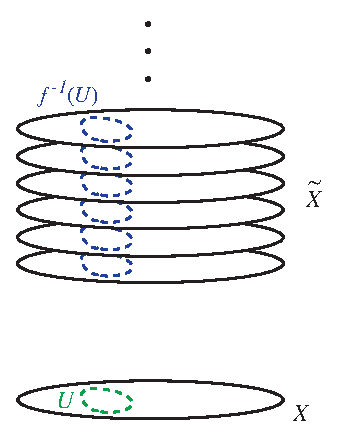
\includegraphics[width=150pt]{images/covering_spaces/D2xN}
\end{figure}
\end{example}

\begin{example}[a non-example]
Let $\tilde{X}=S^1,$ and let $X=S^1 \lor S^1.$  That is, $X$ is two copies of $S^1,$ which agree at a point.  

Let $\sim$ be the equivalence relation on $S^1$ given by $x \sim y$ if and only if $x,y \in \{x_1,x_2\}$ or $x=y$.  Let $p$ the the quotient map from $\tilde{X}$ to $X$, corresponding to this relation, and let $U$ be an open set in $X$ containing $x_1,x_2,$ as shown.  Is $U$ evenly covered?

The answer is no.  To see why, note that $p^{-1}(U)=V_1 \cup V_2,$ where $V_1,V_2$ are disjoint open sets in $\tilde{X}$.  But $p \vert V_1: V_1 \rightarrow U$ is not a homeomorphism because it is not onto.  
\end{example}

\begin{definition}  Let $p: \tilde{X} \twoheadrightarrow X$ be a continuous surjection.  Suppose for all $x \in X$, there exists an evenly covered open set $U$ containing $X$.   We say $p$ is a \textbf{covering map}, $\tilde{X}$ is the \textbf{covering space} and $X$ is the \textbf{base space.}
\end{definition}

\begin{example}[another non-example]
Let $\tilde{X}=\R^2,$ $X=\R,$ and $P:\R^2\rightarrow \R$ be defined by $p(x,y)=x$.  Then for each open $U \subseteq X,$ $p^{-1}(U)=\cup_{\alpha \in A}V_{\alpha}.$  (We can think of $p^{-1}(U)$ as a horizontal stack of uncountably many copies of $U$).  For each $\alpha \in A,$ $p \mid V_{\alpha}: V_{\alpha} \rightarrow U$ is a homeomorphism.  However, each $V_{\alpha}$ is not open in $\tilde{X}$.
\end{example}

\begin{lemma}[Important Lemma on Covering Maps]
Let $p:\tilde{X} \rightarrow X$ be a covering map.  Let $x \in X$.  Then the subspace topology on $p^{-1}(\{x\})$ is the discrete topology.
\end{lemma}

\begin{proof}
Let $y \in p^{-1}(\{x\}).$  We want to show that $\{y\}$ is open in $p^{-1}(\{x\})$.  Since $p$ is a covering map, there exists a evenly covered open set $U$ containing $x$.  Then $p^{-1}(U)=\cup_{\alpha \in A}V_{\alpha}$, where the $V_{\alpha}$ are pairwise-disjoint open sets such that $p \mid V_{\alpha}:V_{\alpha}\rightarrow U$ is a homeomorphism for every $\alpha \in A$.  Hence, there exists $\alpha_0 \in A$ such that $y \in V_{\alpha_0}$.  Now, $V_{\alpha_0}$ is open in $\tilde{X}$.  Note that $y \in V_{\alpha_0}\cap p^{-1}(\{x\})$.  Let $y' \in V_{\alpha_0} \cap p^{-1}(\{x\})$ be given.  We know that $p \mid V_{\alpha_0}$ is a homeomorphism, so it is injective.  Since $p(y')=x,$ and $p(y)=x,$ we see that $y=y'$.  Thus, $\{y\}=V_{\alpha_0} \cap p^{-1}(\{x\})$, both of which are open in $p^{-1}(\{x\}).$ So $\{y\}$ is open in $p^{-1}(\{x\})$ with the subspace topology.  This completes the proof.
\end{proof}

The take-home message is that in a covering space, points in the pre-image of a single point are ``spread out."

\begin{example}[Important] Let $p:\R \rightarrow S^1$ be defined by $p(x)=(\cos(2 \pi x), \sin(2 \pi x))$.  (The ``slinky" space.)

\begin{figure}[ht!]
    \centering
    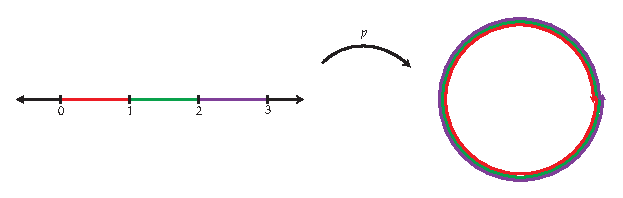
\includegraphics[width=330pt]{images/covering_spaces/slinky}
\end{figure}

For each $s \in S^1,$ an ``open interval" around $s$ is evenly covered, and so $\R$ is a covering space.  
\end{example}

\begin{example}
$\tilde{X}=S^1,$ $X=S^1$ by $p:\tilde{X} \rightarrow X$ is $p((\cos(2 \pi x), \sin(\pi x))=(\cos(4 \pi x), \sin(4 \pi x)).$  

\begin{figure}[ht!]
    \centering
    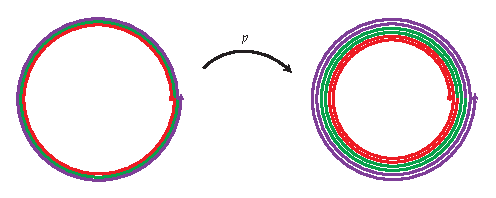
\includegraphics[width=330pt]{images/covering_spaces/s1_to_s1}
\end{figure}
\end{example}

Not all quotient maps are covering maps.  But we will prove that all covering maps are quotient maps.  (Remember our important example?)

\begin{theorem}  Let $p:\tilde{X}\rightarrow X$ be a covering map.  Then
\begin{enumerate}
\item  $p$ is an open map
\item $X$ is a quotient space, and $p$ is a quotient map.
\end{enumerate}
\end{theorem}

\begin{proof}  Let $U$ be open in $\tilde{X}$.  We want to show that $p(U)$ is open.  Let $x \in p(U).$  Then there exists an evenly covered open set $V$ containing $X$.  Now, there exists $y \in U$ such that $p(y)=x.$  Then $p^{-1}(V)=\cup_{\alpha \in A}V_{\alpha}$ such that the $V_{\alpha}$ are disjoint open sets and $p \mid V_{\alpha}$ is a homeomorphism for all $\alpha \in A$.  Let $\alpha_0 \in A$ such that $y \in V_{\alpha_0}$.  There exists such an $\alpha_0$ because $x \in V$.

Because $U$ and $V_{\alpha_0}$ are both open, $U\cap V_{\alpha_0}$ is open in $\widetilde{X}$. Recall $p\mid V_{\alpha_0}:V_{\alpha_0}\rightarrow V$ is a homeomorphism, so 
\begin{align*}
p(U\cap V_{\alpha_0})&=p\left(V_{\alpha_0}\cap p(U)\right)\\
&=V\cap p(U)
\end{align*}
where $V\cap p(U)$ is open in $V$ and $U$ is open in $X$. Therefore, $V\cap p(U)$ is open in $X$. Because our $x$ is in both $V$ and $p(U)$, $x\in V\cap p(U)\subseteq p(U)$. That is, $x$ is an element of an open set contained in $p(U)$. Hence, $p(U)$ is open and $p$ is an open map.
\item To show $X$ has the quotient topology with regard to $p$, we want to show that $F_X = \{U\subseteq X \mid p^{-1}(U)\in F_X\}$.

\begin{itemize}
\item[$(\subseteq)$] Let $V\in F_X$. Because $p$ is continuous, $p^{-1}(V)\in F_{\widetilde{X}}$. Thus, $V\in \{U\subseteq X \mid p^{-1}(U)\in F_X\}$.

\item[$(\supseteq)$] Let $U\subseteq X$ such that $p^{-1}(U)\in F_{\widetilde{X}}$. Because $p$ is open, $p(p^{-1}(U)$ is open in $X$. Because $p$ is onto $p(p^{-1}(U))=U$. Thus, $U\in F_X$.
\end{itemize}

$F_X = \{U\subseteq X \mid p^{-1}(U)\in F_X\}$, so $p$ is a quotient map and $X$ is a quotient space. 

\end{proof}

\newpage
\subsection{Lifts}
\begin{definition}
Let $p:\widetilde{X}\rightarrow X$ be a covering map and $f:Y\rightarrow X$ be continuous. We define a \textit{lift} of $f$ to be any continuous function $\widetilde{f}:Y\rightarrow X$ such that $p\circ \widetilde{f}=f$.
\end{definition}

\begin{example}
Let $\widetilde{X}=\R$, $X=S^1$ and $p(x)=\left(\cos(2\pi x),\sin(2\pi x)\right)$. Let $f:I\rightarrow S^1$ by $f(x)=\left(\cos(\pi x),\sin(\pi x)\right)$. Define $\widetilde{f}:I\rightarrow \R$ by $f(x)=\frac{x}{2}$.

\begin{figure}[ht!]
    \centering
    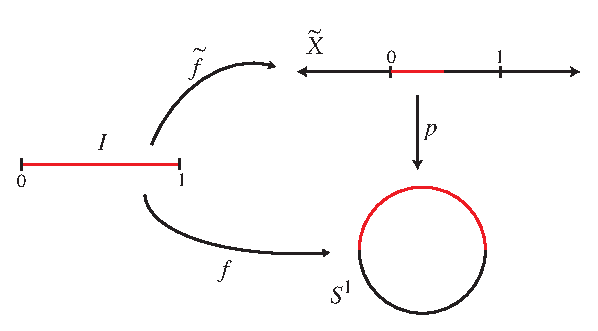
\includegraphics[width=300pt]{images/covering_spaces/s1_lift}
\end{figure}

\end{example}

\begin{lemma}
\textbf{Uniqueness of Lifts.} Let $p:\widetilde{X}\rightarrow X$ be a covering map and $f:Y\rightarrow X$ be a covering and $f:Y\rightarrow X$ be continuous and $Y$ be connected. Let $\widetilde{f_0}$ and $\widetilde{f_1}$ be lifts of $f$. Suppose there exists $y_0\in Y$ such that $\widetilde{f_0}(y_0)=\widetilde{f_1}(y_0)$ then $\widetilde{f_0}=\widetilde{f_1}$.
\end{lemma}
\begin{proof}
Let $Y' =\{y\in Y\mid \widetilde{f_0}(y)=\widetilde{f_1}(y)\}$. $Y\ne\emptyset$. We want to show that $Y' = Y$, we will accomplish by showing $Y'$ is clopen in $Y$. 
\begin{itemize}
\item[Open:] Let $y\in Y'$. There exists an evenly covered open set $V$ containing $f(y)$. $p^{-1}(V)=\displaystyle\bigcup_{\alpha\in A} V_\alpha$ such that $V_{\alpha}$'s are disjoint and open; also, $p\mid V_\alpha:V\alpha\rightarrow V$ is a homeomorphism. 

Let $q= \widetilde{f}_0(y)=\widetilde{f_1}(y)$. There exists and $\alpha_0\in A$ such that $q\in V_{\alpha_0}$. $\widetilde{f}_0^{-1}(V_{\alpha_0})$ and $\widetilde{f}_1^{-1}(V_{\alpha_0})$ are open in $Y$, and $y\in \widetilde{f}_0^{-1}(V_{\alpha_0})\cap\widetilde{f}_1^{-1}(V_{\alpha_0})$.
We claim that $\widetilde{f}_0^{-1}(V_{\alpha_0})\cap\widetilde{f}_1^{-1}(V_{\alpha_0})\subseteq Y'.$

Let $z\in \widetilde{f}_0^{-1}(V_{\alpha_0})\cap\widetilde{f}_1^{-1}(V_{\alpha_0}),$ implying $\widetilde{f_0}(z)\in V_{\alpha_0}$ and $\widetilde{f_1}(z)\in V_{\alpha_0}$. Because $\widetilde{f_0}(z)$ and $\widetilde{f_1}(z)$ are lifts of $f$, $p\circ\widetilde{f_0}(z)=f(z)$ and $p\circ\widetilde{f_1}(z)=f(z)$. Since $p$ is 1-1 (because $p$ is a homeomorphism) and $\widetilde{f_0}(z)\in V_{\alpha_0}$ and $\widetilde{f_1}(z)\in V_{\alpha_0}$, $\widetilde{f_0}(z)=\widetilde{f_1}(z)$. Thus, $z\in Y'$.

Hence, $\widetilde{f}_0^{-1}(V_{\alpha_0})\cap\widetilde{f}_1^{-1}(V_{\alpha_0})$ is an open subset of $Y'$ containing $y$, so $Y'$ is open.
\item[Closed:] To show $Y'$ is closed, we will show $Y-Y'$ is open. Let $y\in Y-Y'$. here exists an evenly covered open set $V$ containing $f(y)$. $p^{-1}(V)=\displaystyle\bigcup_{\alpha\in A} V_\alpha$ such that $V_{\alpha}$'s are disjoint and open; also, $p\mid V_\alpha:V\alpha\rightarrow V$ is a homeomorphism. 

Note that $\widetilde{f}_0(y)\ne\widetilde{f_1}(y)$. There exists and $\alpha_1,\alpha_2\in A$ such that $\widetilde{f}_0(y)\in V_{\alpha_1}$ and $\widetilde{f}_1(y)\in V_{\alpha_2}$. The set $\widetilde{f}_0^{-1}(V_{\alpha_1})\cap\widetilde{f}_1^{-1}(V_{\alpha_2})$ is open and contains $y$. We claim that $\widetilde{f}_0^{-1}(V_{\alpha_1})\cap\widetilde{f}_1^{-1}(V_{\alpha_2})\subseteq Y-Y'$.

Let $z\in \widetilde{f}_0^{-1}(V_{\alpha_1})\cap\widetilde{f}_1^{-1}(V_{\alpha_2}),$ implying $\widetilde{f_0}(z)\in V_{\alpha_1}$ and $\widetilde{f_1}(z)\in V_{\alpha_2}$. We now want to show that $\widetilde{f_0}(z)\ne\widetilde{f_1}(z)$. Recall that $p\mid V_{\alpha_1}$ is $1-1$ and $p\circ\widetilde{f}_0(y)=f(y)=p\circ\widetilde{f}_1(y)$: because $\widetilde{f}_0(y)\ne\widetilde{f}_1(y)$ where $\widetilde{f}_0(y)\in V_{\alpha_1}$ and $\widetilde{f}_1(y)\in V_{\alpha_2}$, implying that $\alpha_1\ne \alpha_2$. Otherwise, $\widetilde{f}_0(y)$ and $\widetilde{f}_1(y)$ would be two points in $V_{\alpha_1}$ that both map to $f(y)$. Therefore, $V_{\alpha_1}\cap V_{\alpha_2}=\emptyset$.

Therefore $\widetilde{f_0}(z)\ne\widetilde{f_1}(z)$, implying that $z\in Y-Y'$. This implies $y$ is contained in the open set $\widetilde{f}_0^{-1}(V_{\alpha_1})\cap\widetilde{f}_1^{-1}(V_{\alpha_2})\subseteq Y-Y'$, making $Y-Y'$ open. 
\end{itemize}
Therefore $Y'$ is clopen in $Y$. Because $Y'$ is non-empty and $Y$ is connected, $Y'$ must be all of $Y$. By the definition of $Y'$, $\widetilde{f_0}=\widetilde{f_1}$.
\end{proof}


    \begin{lemma}[Lebesgue Number Lemma]
    Let $X$ be a compact metric space and let $\Omega$ be an open cover of $X$. Then $\exists$ $r > 0$ such that $\forall$ $A \subseteq X$ with $lub \{ d(p,q)|p, q \in A \} < r$, $A$ is contained in a single element of $\Omega$.
    
    ($r$ is said to be a Lebesgue Number for $\Omega$)
    \end{lemma}
    
    We will now use this to prove the existence of lifts.
    \begin{theorem}[Very Important Homotopy Path Lifting Theorem]
    Let $p: \widetilde{X} \to X$ be a covering map. Then,
    \begin{enumerate}
\item Given a path $f$ in $X$ and $a \in \widetilde{X}$ such that $p(a) = f(0)$, then $\exists !$ (exists unique) path $\widetilde{f}$ in $\widetilde{X}$ such that $p \circ \widetilde{f} = f$ and $\widetilde{f}(0) = a$.
\item Given a continuous map $F: I \times I \to X$ and $a \in \widetilde{X}$ with $p(a) = f(0,0)$, $\exists !$ continuous map $\widetilde{F}$$\colon I \times I \to \widetilde{X}$ such that $p \circ \widetilde{F} = F$ and $\widetilde{F}(0,0) = a$.
\end{enumerate}
\end{theorem}
    \begin{proof}
    \begin{enumerate}
    \item $\forall$ $x \in f(I),$ $\exists$ $V_x$ an evenly covered open set containing $x$. $\forall$ $x \in f(I)$, $f^{-1}(V_x)$ is open in $I$, so $\{f^{-1}(V_x)|x \in f(I) \}$ is an open cover of $I$. So, $\exists$ Lebesgue number $r$ for this cover. $\exists$ $n \in \N$ such that $\tfrac{1}{n} < r$.  $\forall$ $k \leq n$, $[ \frac{k-1}{n}, \frac{k}{n}]$ is contained entirely in some $f^{-1}(V_x)$. So, $\exists$ $\{ V_1, V_2, ... , V_n \} \subseteq \{ V_x \}$ such that $\forall$ $k \leq n$, $f([ \frac{k-1}{n}, \frac{k}{n}]) \subseteq V_k$.
    First, $V_1$ is evenly covered and $f(0) \in V_1$, so $a \in p^{-1}(V_1) = \bigcup_{ \alpha \in A_1}V_{\alpha}$. So, $\exists$ $\alpha_1 \in A_1$ such that $a \in V_{\alpha_1}$. $p | V_{\alpha_1}\colon$ $V_{\alpha_1} \to V_1$ is a homeomorphism. So $\forall$ $s \in [0, \tfrac{1}{n}]$, define $\widetilde{f}(s) = (p | V_{\alpha_1})^{-1} f(s)$. Note that $\widetilde{f} \colon$ $[0, \tfrac{1}{n}] \to \widetilde{X}$ continuous because $(p | V_{\alpha_1})^{-1}$ is a homeomorphism.
    Now note that, as above, $p^{-1}(V_2) =  \bigcup_{ \alpha \in A_2}V_{\alpha}$. $f(\tfrac{1}{n}) \in V_2$ by definition. $\exists$ $\alpha_2 \in A_2$ such that $\widetilde{f}(\tfrac{1}{n}) \in V_{\alpha_2}$. So, as above, define $\widetilde{f} \colon$ $[\tfrac{1}{n}, \tfrac{2}{n}] \to \widetilde{X}$ by $\widetilde{f}(s) = (p | V_{\alpha_2})^{-1} f(s)$. $\widetilde{f} \colon$ $[0, \tfrac{2}{n}] \to \widetilde{X}$ is therefore continuous by Pasting Lemma.
    	
    
    \item  $\forall x \in F(I \times I)$ $\exists$ evenly covered open set $V_x$. $\{ F^{-1}(V_x) \}$ is an open cover of $I \times I$, so it has a Lesbegue number $r$. $\exists$ $n > \tfrac{\sqrt{2}}{r}$. $\forall$ $i \leq n$, let $A_i = [\tfrac{i-1}{n}, \tfrac{i}{n}]$, $B_i = [\tfrac{i-1}{n}, \tfrac{i}{n}]$. $\forall$ $i, j$, $F(A_i \times B_j) \subseteq V_{ij}$ for some $V_{ij} \in \{ V_x \}$. By Part 1, we can lift $F|(I \times \{ 0 \} \cup \{ 0 \} \times I)$ to $\widetilde{F} \colon$ $(I \times \{ 0 \} \cup \{ 0 \} \times I) \to \widetilde{X}$ such that $\widetilde{F}(0,0) = a \in \widetilde{X}$.

Begin by observing that $V_{11}$ is evenly covered by hypothesis, and $F(I_1\times J_1)\subseteq V_{11}$. This means that $p^{-1}(V_{11})=\bigcup_{\alpha \in A_{11}}V_\alpha$ where the $V_\alpha$ are disjoint open sets and $A_{11}$ is some index set. Since $F(0,0)\in V_{11}$, and since $\tilde{F}(0,0)=a$, it follows that there exists some $\alpha_{11}\in A_{11}$ such that $a\in V_{\alpha_ {11}}$.

	Now we worry that this choice of $V_{\alpha_{11}}$ will agree with how we defined $\tilde{F}$ on the set $L$. Worry not! For $L$ is connected, and $L\cap (I_1\times J_1)$ is connected, and since $\tilde{F}$ is continuous, $\tilde{F}(L\cap (I_1\times J_1))$ is connected. Since the $V_\alpha$ are open and disjoint, we may therefore conclude that $\tilde{F}(L\cap (I_1\times J_1))\subseteq V_{\alpha_{11}}$ (otherwise it would be disconnected).

	Since $V_11$ was evenly covered, we know that $p\mid V_{\alpha_{11}}$ is a homeomorphism, so we may define $\tilde{F}\colon I_1\times J_1\to \tilde{X}$ by:
	\[ \tilde{F}(s,t)=(p\mid V_{\alpha_{11}})^{-1}\circ F(s,t) \]
	This is a composition of continuous functions, so is continuous. Furthermore, $\tilde{F}\colon L\cup (I_1\times J_1)\to \tilde{X}$ is continuous since we showed that $\tilde{F}(L\cap (I_1\times J_1))\subseteq V_{\alpha_{11}}$, so we apply the Pasting Lemma.

    Now we want to extend $\tilde{F}$ to the rest of $I\times I$, and so we move to $I_2\times J_1$. Here we have an analogous situation as before: We want to choose the appropriate $V_\alpha$ associated with $V_{21}$ so that our extension of $\tilde{F}$ agrees with what we had previously. But again, $\tilde{F}((I_2\times J_1)\cap (L\cup (I_1\times J_1)))$ is connected, so following the argument from above there will be an appropriate choice of $V\alpha$ to make it ``work''. So we inductively define $\tilde{F}\colon I\times I\to \tilde{X}$ such that it is continuous as before, and $p\circ \tilde{F}=F$ and $\tilde{F}(0,0)=a$. That $\tilde{F}$ is unique follows from our Uniqueness of Lifts Lemma above.
    \end{enumerate}

We iterate this argument finitely many times for each tile $I_i\times J_j$, and so inductively define a unique lift of $F$: $\tilde{F}\colon I\times I\to \tilde{X}$ such that $\tilde{F}(0,0)=a$.
  \end{proof}


  The natural intuition is that our new function $\tilde{F}$ is a path homotopy when $F$ is a path homotopy. This intuition provides a delightful segue to the next theorem:
  \begin{theorem}[Monodromy Theorem]
  Let $p: \tilde{X}\to X$ be a covering map, and let $a\in \tilde{X}$. Let $x_1,x_2\in X$. Suppose that $p(a)=x_1$, and that $f,g$ are paths in $X$ from $x_1$ to $x_2$. Let $\tilde{f}, \tilde{g}$ be the unique lifts of $f,g$ beginning at $a$. Then if $f\sim g$, $\tilde{f}(1)=\tilde{g}(1)$ and $\tilde{f}\sim \tilde{g}$.
  \end{theorem}
   Before beginning the proof, we observe with relish the etymology of monodromy. Mono being the prefix for one, and dromy being some sort of Greek for a race track. E.g. hippodrome, airdrome, palindrome (examples courtesy of dictionary.com). Let us race towards the proof!
    \begin{proof}
    $f\sim g$ means that there exists a path homotopy $F\colon I\times I\to X$, and so by the previous theorem there exists a unique lifting of $F$, whose name is $\tilde{F}\colon I\times I\to \tilde{X}$, and $\tilde{F}$ has the property that $\tilde{F}(0,0)=a$ and $p\circ \tilde{F}=F$. Now $\tilde{f}, \tilde{g}$ are lifts of $f,g$ respectively. Consider $\tilde{F}\mid (I\times \left\{0\right\})$. This is a path in $\tilde{X}$ from $a$ to $\tilde{F}(1,0)$. Observe that:
    \[p\circ \tilde{F}\mid (I\times \left\{0\right\})=F\mid (I\times \left\{0\right\})=f \]
since $F$ was a path homotopy, and on the other hand:
	\[p\circ \tilde{F}\mid (I\times \left\{1\right\})=F\mid (I\times \left\{1\right\})=g\]
The first observation allows us to conclude that $\tilde{F}\mid (I\times \left\{0\right\})$ is a lift of $f$ beginning at $a$. By the uniqueness of lifts, we conclude that $\tilde{F}\mid (I\times \left\{0\right\})=\tilde{f}$. We want to say the same for $\tilde{F}\mid (I\times \left\{1\right\})$, but we do not know that $\tilde{F}(0,1)=a$, so we cannot immediately conclude that this is equal to $\tilde{g}$ since it could possibly be a lift of $g$ originating at some other point.

We claim: $\tilde{F}\mid (\left\{0\right\} \times I)=a$. To see that this is the case, we know:
	\[p\circ \tilde{F}\mid (\left\{0\right\} \times I)=F\mid(\left\{0\right\} \times I)=x_1.\]
    which implies that
	\[\tilde{F}\mid (\left\{0\right\} \times I)\subseteq p^{-1}(F\mid (\left\{0\right\} \times I)=p^{-1}(x_1)\]

    Now we know that since $p$ is a covering map, $p^{-1}(x_1)$ has the discrete topology. Also, $\tilde{F} (\left\{0\right\} \times I)$ is connected, so must contain only a single point of $p^{-1}(x_1)$. Certainly $a\in \tilde{F}(\left\{0\right\} \times I)$, so we may say that $a=\tilde{F}(\left\{0\right\} \times I)$ as desired.

    The previous consideration tells us that $\tilde{F}\mid (I\times \left\{1\right\})=\tilde{g}$, since the left hand side is a lift of $g$ originating at $a$, and by the uniqueness of lifts this must be $\tilde{g}$. To finish off proving that $\tilde{F}$ is a path homotopy, we need to show that the endpoints are constant as well. That is, we want to show that $\tilde{F}(\left\{1\right\} \times I)=a'$ for some $a'\in \tilde{X}$. But for this, the same argument as above applies, replacing every instance of $x_1$ with $x_2$. So we conclude that: 
    
	\[\tilde{F}(1,0)=\tilde{f}(1)=\tilde{g}(1)=\tilde{F}(1,1)\]
	
    which was part of what we were trying to prove. All these considerations together tell us that $\tilde{F}$ is a path homotopy between $\tilde f$ and $\tilde{g}$, so $\tilde{f}\sim \tilde{g}$ and we are done.
    \end{proof}
    
    \subsection{$S^1$ and $\Z$}
   	Apparently our ultimate goal is to prove that the fundamental group of $S^1$ is isomorphic to $\Z$ (with addition). But we need just a teensy bit more machinery, and introduce a new function.
   	\begin{definition}
   	Let $p: \mathbb{R}\to S^1$ be the covering map $p(x)=(\cos 2\pi x, \sin 2\pi x)$. Let $x_0=(1,0)$, let $f$ be a loop in $S^1$ with base point $x_0$. Define the \textbf{degree} of $f$, denoted $deg(f)$, as $\tilde{f}(1)$ where $\tilde{f}$ is the unique lift of $f$ starting at $0$.
   	\end{definition}
        
    First, observe that $deg(f)$ is well defined. That is, it doesn't matter which lift we select, because there is only one lift! Also, convince yourself that $p^{-1}(\left\{x_0\right\})=\Z$.
    
This leads us to the theorem we have been clamoring for:

\begin{theorem}
Let $x_0\in S^1$. Then $\pi_1(S^1,x_0)\cong (\mathbb{Z},+)$.
\end{theorem}

\begin{proof}
We assume WLOG that $x_0=(1,0)$ since $S^1$ is simply connected. Let $\phi \colon \pi_1(S^1,s_0)\to \Z$ by $\phi([f])=deg(f)$. Recall from last lecture that we defined $deg(f)=\tilde{f}(1)$ where $\tilde{f}$ was the lift of $f$ based at $0$ with respect to the covering map $p\colon \R\to S^1$ defined by $p(x)=(\cos 2\pi x, \sin 2\pi x)$. Our aim is to show that $\phi$ is an isomorphism.

\begin{itemize}
\item[Well-Defined:]
Suppose $[f]=[g]$. Then $f\sim g$ are homotopic loops in $S^1$ based at $x_0$. By the Monodromy theorem, we may say that $\tilde{f}(1)=\tilde{g}(1)$ (from here on out we assume that $\tilde{f},\tilde{g}$ are the lifts of $f,g$ respectively based at $0$). This implies that $deg(f)=deg(g)$, which means that $\phi([f])=\phi([g])$ and so $\phi$ is well-defined.

\item[1-1:]
Let $[f],[g]\in \pi_1(S^1,x_0)$ be such that $\phi([f])=\phi([g])$. This means that $deg(f)=deg(g)$, and this means that $\tilde{f}(1)=\tilde{g}(1)$. But $\mathbb{R}$ is simply connected, so since $\tilde{f},\tilde{g}$ share an endpoint we may say that $\overline{\tilde{f}}\sim \overline{\tilde{g}}$, and there exists a path homotopy $\tilde{F}\colon I\times I\to \mathbb{R}$ such that $\tilde{F}(0,t)=\overline{\tilde{f}}$ and $\tilde{F}(1,t)=\overline{\tilde{g}}$. Consider $p\circ \tilde{F}$. This is continuous because it is a composition of continuous functions, and $p\circ \tilde{F}(0,t)=p\circ \overline{\tilde{f}}=\overline{f}$; $p\circ \tilde{F}(1,t)=p\circ \overline{\tilde{g}}=\overline{g}$. Finally, we know that for all $s\in I$ we have $\tilde{F}(s,0)=\tilde{f}(1)$, so $p\circ \tilde{F}(s,0)=p\circ \tilde{f}(1)=f(1)=x_0$, and the same goes for $t=1$, so $p\circ \tilde{F}$ goes to a loop homotopy $F$ which takes $\overline{f}$ to $\overline{g}$, but since these are loops we may deduce that $f\sim g$. This means that $[f]=[g]$ and we are done with proving one to one.

\item[Onto:]
Let $n\in \mathbb{Z}$. Since $\mathbb{R}$ is path connected there exists a path $\tilde{f}$ from $0$ to $n$. Then $p\circ \tilde{f}$ is a loop in $S^1$ based at $x_0$ (since $p(\cos 2\pi n, \sin 2\pi n)=(1,0)=x_0$), and $deg(p\circ \tilde{f})=n$. Therefore $\phi([p\circ \tilde{f}])=n$. This proves that $\phi$ is onto.

\item[Homo:]
Let $[f],[g]\in \pi_1(S^1, x_0)$. We want to show that $\phi([f][g])=\phi([f])+\phi([g])$, and the right hand side is equal to $deg(f)+deg(g)$, while the left hand side is equal to $deg(f\ast g)$. So we want to show that $deg(f\ast g)=deg(f)+deg(g)$. Let $\widetilde{f\ast g}$ be the lift of $f\ast g$ beginning at $0$. We want to show that $\widetilde{f\ast g}(1)=\tilde{f}(1)+\tilde{g}(1)$. Let $m=\tilde{f}(1), n=\tilde{g}(1)$. Let us define a function $h\colon I\to \mathbb{R}$ by:
	\[h(s)=\begin{cases}
	\tilde{f}(2s) & s\in [0,\frac{1}{2}]\\
	\tilde{g}(2s-1)+m & s\in [\frac{1}{2},1]
	\end{cases}
\]
Now $h$ is a path in $\mathbb{R}$ from $0$ to $m+n$. This is because $\tilde{f}, \tilde{g}$ are continuous, and when $s=\frac{1}{2}$ we have $\tilde{f}(1)=m$, and $\tilde{g}(0)+m=0+m=m$, so this is continuous by the pasting lemma. Also, $h(0)=0$ and $h(1)=\tilde{g}(1)+m=n+m$. Also we know:
	\[p\circ h(s)=\begin{cases}
	f(2s) & s\in [0,\frac{1}{2}\\
	p(\tilde{g}(2s-1)+m) & s\in [\frac{1}{2},1]
	\end{cases}
\]
Now observe that the second half of this is:
\begin{align*}
	p(\tilde{g}(2s+1)+m)&=(\cos 2\pi (\tilde{g}(2s-1)+m), \sin2\pi (\tilde{g}(2s-1)+m))\\
											&=(\cos 2\pi \tilde{g}(2s-1),\sin2\pi \tilde{g}(2s-1))\\
											&=p(\tilde{g}(2s-1))\\
											&=g(2s-1)						
\end{align*}
\end{itemize}
Thus we see that $p\circ h=f\ast g$, which implies that $h=\widetilde{f\ast g}$ since $h$ begins at $0$ and we know that lifts are unique w/r/t their starting points. Now $h(1)=m+n=\tilde{f}(1)+\tilde{g}(1)$, so putting it together:
	\[deg(f\ast g)=deg(f)+deg(g)\Rightarrow \phi([f][g])=\phi([f])+\phi([g])\]
So we conclude that $\phi$ is a homomorphism. This plus one to one and onto means that $\phi$ is in fact an isomorphism, so we conclude that $\mathbb{Z}\cong \pi_1(S^1,x_0)$.
\end{proof}
We rejoice at the fact that we have now seen a non trivial fundamental group. 

\subsection{More \textit{Fun}damental Groups}
 Check out this theorem:
\begin{theorem}
Let $x_0\in X$ and $p\colon \tilde{X}\to X$ be a covering map. If $\tilde{X}$ is simply connected, then there exists a bijection from $\pi_1(X,x_0)$ to $p^{-1}(\left\{x_0\right\})$.
\end{theorem}
\begin{proof}
We only needed simple connectedness in the proof that $\phi$ was $1-1$ and onto, so we use an analogous proof to show that $\phi \colon \pi_1(X,x_0)\to p^{-1}(\left\{x_0\right\})$ by $\phi([f])=\tilde{f}(1)$, where $\tilde{f}$ is the unique lift originating at some $y_0\in p^{-1}(\left\{x_0\right\})$. 
\end{proof}

\begin{theorem}
Let $p\colon S^2\to \mathbb{R}P^2$ be the quotient map. Then $p$ is a covering map.
\end{theorem}
\begin{proof}
Recall that the equivalence relation for this quotient map was defined as $x\sim y$ iff $x=\pm y$. We use one of the most powerful proof techniques known to mathematics here: proof by picture. Consider any open ball in $\mathbb{R}P^2$ containing some point. Then its pre image will be a pair of disjoint balls such that $p$ restricted to the balls will be a homeomorphism. Just think about it... or look at the pictures below.

\begin{figure}[ht!]
    \centering
    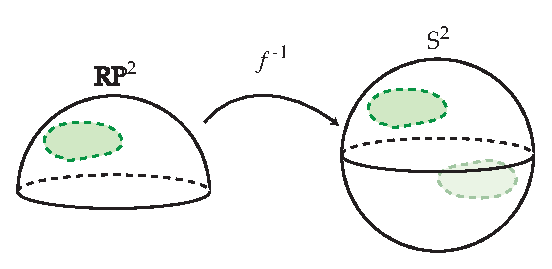
\includegraphics[width=300pt]{images/covering_spaces/rp2_quotient}
\end{figure}
\end{proof}

$\mathbb{R}P^2$ provides us with another example of a space with a nontrivial fundamental group. From one of our theorems, we know that given $x_0\in \mathbb{R}P^2$ there is a bijection from $\pi_1(\mathbb{R}P^2,x_0)$ to $p^{-1}(\left\{x_0\right\})$ (since $\mathbb{R}P^2$ is simply connected), and we know that $p^{-1}(\left\{x_0\right\})$ has precisely two elements, so $\pi_1(\mathbb{R}P^2,x_0)\cong \mathbb{Z}_2$ (alternatively written by algebraists as $\mathbb{Z}/ 2\mathbb{Z}$).


\section{$\R^2 \not\cong\R^3$}
\begin{theorem} $\R^2 \not \cong \R^3$\end{theorem}
\begin{proof}
First, recall some previous results:
\begin{itemize}
\item $\R^{n+1} \setminus \{p\}$ is homotopy equivalent to $S^n$
\item $\pi_1(S^2, x_0)$ is trivial
\item $\pi_1(S^1, x_0) \cong \Z$
\end{itemize}

Now suppose that $\R^2 \cong \R^3$.  Then there exists some homeomorphism $h : \R^2 \to \R^3$.  

Let $p \in \R^2$ and $h(p) = q \in \R^3$.  Therefore $f = h|_{\R^2\setminus\{p\}} :\R^2\setminus\{p\} \to \R^3\setminus\{q\}$ is a homeomorphism. Also, from the previous results:
\begin{itemize}
\item $\pi_1(\R^2 \setminus \{p\}, x_0) \cong \pi_1(S^1, y_0) \cong \Z$
\item $\pi_1(\R^3, \setminus \{q\}, z_0) \cong \pi_1(S^2, w_0) \cong \{1\}$
\end{itemize}
But $f$ is a homeomorphism, so $f_* : \pi_1(\R^2 \setminus \{p\}, x_0) \to \pi_1(\R^3, \setminus \{q\}, z_0)$ is an isomorphism.  However, $\Z \not \cong \{1\}$, so this is a contradiction.  

Therefore $\R^2 \not \cong \R^3$, as desired.
\end{proof}

\section{One Last Thought}
\begin{example}[Not all Fundamental Groups are Abelian]
Let $X = S^1 \vee S^1$ with wedge point $x_0$.  Then $\pi_1(X, x_0)$ is not abelian.
\end{example}
\begin{proof}
Define $Y \subseteq \R^2$ as $Y = \{ (x,y) \mid x = 0 \text{ and/or } y = 0\}$.

Define $\widetilde{X}$ as $Y$ with a copy of $S^1$ wedged at every $(z,0)$ and $(0,z)$ with $z \in \Z \setminus \{0\}$

Define $p : \widetilde{X} \to X$ such that $(x,0)$ goes to the first copy of $S^1$ for all $x \in \R$, $(0,x)$ goes to the second, and $(z,0)$, $(0,z)$ goes to $x_0$ for all $z \in \Z$.  Copies of $S^1$ wedged at $(z,0)$ go with the usual projection to the second copy of $S^1$ in $X$, and the copies wedged at $(0,z)$ go the the first copy in $X$, as show in the image.

\begin{figure}[ht!]
\begin{center}
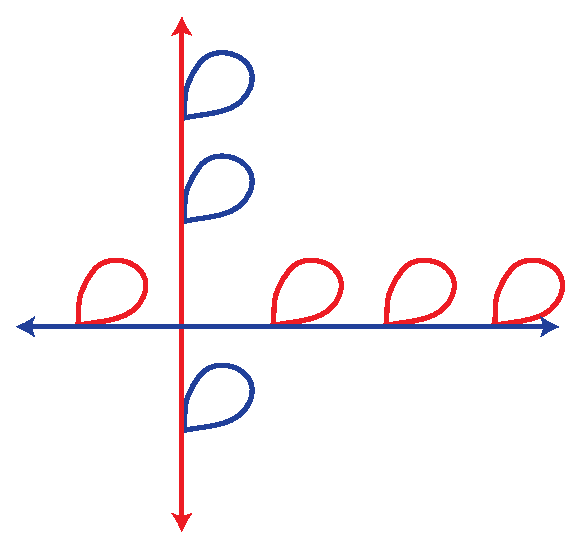
\includegraphics[width=240pt]{images/covering_spaces/nonabelian}
\caption{Blue maps to the first circle, red to the second, and the black squares to $x_0$.}
\end{center}
\end{figure}

Now define $\widetilde{f}(t) = (t,0)$, $\widetilde{g}(t) = (0,t)$, and $f = p \circ \widetilde{f}$, $g = p \circ \widetilde{g}$.  So $f$ is a single loop on the first circle and $g$ is a single loop on the second circle.

Next, lift $f * g$ and $g * f$ at the origin.  The construction of $\widetilde{X}$ gives that $\widetilde{f * g}(1) = (1,0)$ and $\widetilde{g * f}(1) = (0,1)$.  So, by the Monodromy theorem, as this are lifts with the same fixed point, $f * g \not \sim g * f$.  Therefore $[f]$ and $[g]$ satisfy $[f],[g] \in \pi_1(X,x_0)$ and $[f][g] \neq [g][f]$, so $\pi_1(X,x_0)$ is not abelian, as desired.

\end{proof}

Well, that's everything there is to know about topology.  




\end{document} 
